% !TeX spellcheck = de_CH
\documentclass[11pt,a4paper,english,oneside]{book}

\usepackage{etex} %Because of many packages --> Extended TeX.
\usepackage[left=1in, right=1in]{geometry} %Helps to structure the paper layout.
\usepackage[Lenny]{fncychap} %Design of the thesis.
\usepackage[utf8]{inputenc} %Due to vowels.
\usepackage[T1]{fontenc}
\usepackage[ngerman]{babel} %Define the language style.

% german language for appendix header
\addto\captionsngerman{\let\appendixtocname\appendixname%
	\let\appendixpagename\appendixname}

% Setup glossary and acronyms
\usepackage[acronym,toc,nopostdot]{glossaries}
\loadglsentries{glossar-terms}
\glsenablehyper
\makeglossaries

% Include external pdf
\usepackage{pdfpages}

% Float images
\usepackage{wrapfig}


% set single pages to landscape
\usepackage{lscape}

\usepackage{dsfont} %Nice style for the indicator function.
\usepackage{fancyhdr} %To customize the headers and footers.
\usepackage{booktabs} %In case you need \cmidrule or \addlinespace in tables.
\usepackage[hang,bottom,stable,multiple]{footmisc} %Style of footnotes.
\usepackage{appendix} %For the \appendixpage command.
%Load some mathematical packages.
\usepackage{amsmath}
\usepackage{amsfonts}
\usepackage{amsmath}
\usepackage{amssymb}
\usepackage{mathtools}
\usepackage[
backend=biber,
style=numeric,
sortlocale=de_CH,
natbib=true,
doi=true,
eprint=false
]{biblatex}  % Bibliography
\addbibresource{References.bib}
\usepackage{etoolbox} %To remove the page number on \appendixpage.
\usepackage{amsthm} %For theorems, definitions etc.
\usepackage{thmtools} %For theorems, definitions etc.
\usepackage{setspace} %Use double spacing.
\usepackage{lipsum} %For the \lipsum command to generate a text.
\usepackage{datetime} %For the specification of the date.
%\usepackage{tocloft} %The ToC, LoF and LoT each appear not necessarily on a new page.
\usepackage{graphicx,listings,xcolor,textcomp} %For the graphics, listings etc.
\usepackage{mcode} %To implement a Matlab code.
\usepackage[margin=10pt, font=small, labelfont=bf, labelsep=endash]{caption} %Customize the captions.
\usepackage{chngcntr} %To use counterwithout.
\usepackage{epstopdf} %For inserting .eps files into the document.
\usepackage{hyperref} %Must be loaded at the end.
\usepackage{xparse} %Load for \NewDocumentCommand command.
\usepackage{cleveref} %For the command \cref, load after hyperref.
\usepackage{arydshln} %Due to the capability to draw horizontal/vertical dash-lines.
\usepackage{array,hhline} %To create tables and matrices.
\usepackage{rotating} %To rotate a table.
\usepackage{dcolumn, tabularx, multirow} %An extended version of tabular.
\renewcommand{\arraystretch}{1.25}

%Setup of the reference links.
\hypersetup{
	colorlinks=true,
	linkcolor=cyan,
	anchorcolor=black,
	citecolor=cyan,
	filecolor=cyan,
	urlcolor=cyan,
	runcolor=cyan,
	menucolor=black
}


%Define some reasonable margins.
\setlength{\textwidth}{6.6in}
\setlength{\textheight}{8.8in}
\setlength{\topmargin}{-0.1in}
\setlength{\oddsidemargin}{0in}
\setlength{\parskip}{1mm}


\allowdisplaybreaks[1] %Page breaks of equations are allowed, but avoided if possible. 2-4 more relaxed.

%New command for the HSR logo.
\newcommand*{\plogo}{
\includegraphics{logo_hsr.pdf}}

%New command for the differential d to have an ordinary d.
\makeatletter
\newcommand{\ud}{\mathrm{d}}
\makeatother

%Remove page number on \appendixpage. Use the package 'etoolbox'.
\makeatletter
\patchcmd{\@chap@pppage}{\thispagestyle{plain}}{\thispagestyle{empty}}{}{}
\makeatother

%Declare Definitions, Theorems etc.
%%%%%%%%%%%%%%%%%%%%%%%%%%%%%%%%%%%%%%%%%%%%%%%%%%%%%%%%%%%%%%%%%%%%%%%%%%%%%%%%%%%%%%%%%%%%%%%%%%%%%%%%%%%%%%%%%%%
\declaretheorem[style=definition,qed=$\blacktriangleleft$, numberwithin=chapter]{remark} %additional options; numberwithin=,..., see 'Thmtools' Users’ Guide
\declaretheorem[style=definition,qed=$\triangle$,numberwithin=chapter]{definition}
\newtheorem{ass}{Assumption}[chapter]
\newtheorem{prop}{Proposition}[chapter]
\newtheorem{lemma}{Lemma}[chapter]
\declaretheorem[style=definition,qed=$\perp$,numberwithin=chapter]{example}
\newtheorem{theorem}{Theorem}[chapter]
\newtheorem{coroll}{Corollary}[chapter]
%%%%%%%%%%%%%%%%%%%%%%%%%%%%%%%%%%%%%%%%%%%%%%%%%%%%%%%%%%%%%%%%%%%%%%%%%%%%%%%%%%%%%%%%%%%%%%%%%%%%%%%%%%%%%%%%%%%

%Readjust the numbering.
\counterwithout{footnote}{chapter}
\numberwithin{equation}{chapter}


%\setlength{\parindent}{0cm} %Uncomment this if you don't want to have indents.

%----------------------------------------------------------------------------------------
%	TITLE PAGE
%----------------------------------------------------------------------------------------
\newcommand*{\titleGP}{\begingroup %Create the command for including the title page in the document.
	\centering %Center all text.
	\vspace*{\baselineskip} %White space at the top of the page.
	\plogo\\[2\baselineskip] %University Logo.
	\rule{\textwidth}{1.6pt}\vspace*{-\baselineskip}\vspace*{2pt} %Thick horizontal line.
	\rule{\textwidth}{0.4pt}\\[\baselineskip] %Thin horizontal line.
	{\LARGE Graphs-Visualization-Service GVS 2.0 }\\[0.2\baselineskip] %Title.
	\rule{\textwidth}{0.4pt}\vspace*{-\baselineskip}\vspace{3.2pt} %Thin horizontal line.
	\rule{\textwidth}{1.6pt}\\[2\baselineskip] %Thick horizontal line.
	\scshape %Small caps.
	\large Studienarbeit \\[2\baselineskip]
	Abteilung Informatik \par
	Hochschule für Technik Rapperswil
	\vspace*{2\baselineskip}
	
	
	Autoren\\
	{\Large  Michael Wieland  \\ [5pt]}
	
	{\Large Murièle Trentini \\ [5pt]}
	
	\vspace*{2\baselineskip}
	Betreuer\\
	{\Large Thomas Letsch  \\[5pt]
		\small Dozent für Informatik an der \\[5pt]Hochschule für Technik Rapperswil\par}
	\vspace*{2\baselineskip}
	
	\vfill
	{\scshape Zeitraum: 18.09.2017 - 22.12.2017} \\[0.3\baselineskip]
	\endgroup}


%Special header and footer style for the executive summary and Task Assignment section.
\fancypagestyle{firststyle}{%
	\fancyhf{}%
	\renewcommand{\headrulewidth}{0pt}
	\fancyfoot[L]{GVS 2.0}
	\fancyfoot[R]{\thepage}}

% customize header and footer for chapter pages
\fancypagestyle{plain}{
	\fancyhf{}
	\fancyfoot[L]{GVS 2.0}
	\fancyfoot[R]{\thepage}
	\renewcommand{\headrulewidth}{0pt}% Line at the header invisible
	\renewcommand{\footrulewidth}{0pt}% Line at the footer visible
}

%Customize headers and footers for normal pages
\pagestyle{fancy}
\fancyhead[R]{Murièle Trentini | Michael Wieland}
\fancyhead[L]{\rightmark}
\fancyfoot[L]{GVS 2.0}
\fancyfoot[C]{}
\fancyfoot[R]{\thepage}

%Define the signature line with dots.
\NewDocumentCommand \dotbox {o O{.5\linewidth} m O{3ex} O{\linewidth}}
{
	\begin{minipage}{7cm}
		\makebox[7cm][l]{\,.\dotfill}
		\\
		\makebox[7cm][l]{\,#3}
	\end{minipage}
}

\begin{document}
	\thispagestyle{empty}
	\titleGP
	\newpage
	\doublespacing
	\setcounter{page}{1}
	\pagenumbering{Roman}
	\section*{Abstract}
	\thispagestyle{firststyle}
	An der \gls{hsr} werden in den Modulen \textit{Algorithmen und Datenstrukturen 1 und 2} diverse Algorithmen unterrichtet, die auf den beiden Datenstrukturen \textit{Graph} und \textit{Tree} arbeiten. Die Funktionsweise solcher Algorithmen ist für Studenten teilweise schwer zu verstehen. Hinzu kommt, dass die Programmierung für die Visualisierung der Algorithmen mit viel Aufwand verbunden ist. Aus diesen Gründen wurde im Jahr 2005, im Rahmen einer Diplomarbeit, der \gls{gvs} 1.0 entwickelt. Der GVS besteht aus einer clientseitigen Software-Bibliothek, sowie einer Server Komponente, welche die eingehenden Datenstrukturen visualisiert. So können Studenten die Arbeitsweise der Algorithmen Schritt für Schritt nachvollziehen. \\
	
	%TODO: Allenfalls in Vergangenheits Form wechseln!
	\noindent Diese Studienarbeit beschäftigt sich mit der Erneuerung des GVS 1.0, wobei insbesondere bei der Server Komponente das UI Framework mit \gls{javafx} ersetzt wird. In der Analysephase wird die Funktionsweise des Vorgängerprodukts untersucht und Vorschläge für Verbesserungen gemacht. Die gewonnenen Erkenntnisse fliessen in eine klare Schichtenarchitektur ein, die es auch Folgearbeiten erleichtern wird, einzelne Schichten zu ersetzen. Ebenfalls halten aktuelle Software Best Practices wie Dependency Injection im Projekt Einzug. \\

	\noindent Während dem Projekt konnte eine erweiterbare Software Architektur erstellt werden, die das Vorgängerprodukt vollständig ersetzt. In den eingesetzten Metriken ist klar ersichtlich, dass sich die Code-Qualität über die Dauer des Projekts stark verbessert hat. Zusätzlich profitiert der GVS von einem modernen, intuitiven User Interface, das \textit{Graphen} und \textit{Trees} durch den Einsatz von speziellen Layouting Algorithmen ansprechend darstellt.
	
	\newpage
	
	\section*{Management Summary}
	\thispagestyle{firststyle}
	%TODO: Allenfalls in Vergangenheits Form wechseln!
	\subsection*{Ausgangslage}
	\gls{gvs} ist eine Visualisierungs-Software, die Graphen und Trees darstellt. Zusätzlich wird die Arbeitsweise von Algorithmen durch den Einsatz von Farben und gerichteten Kanten visuell hervorgehoben. \\
	Die Datenstrukturen werden in der Entwicklungsumgebung des Benutzers implementiert und mit einer clientseitigen Library an die Visualisierungskomponente übertragen. Dort werden die eingehenden Daten interpretiert und auf eine ansprechende Art und Weise dargestellt. \\
	
	\noindent
	Der im Jahre 2005 entwickelte GVS 1.0 wurde im Unterricht der Module \textit{Algorithmen und Datenstrukturen 1 und 2} aktiv verwendet. Er erleichtert das Erlernen von komplexen Suchalgorithmen und Datenstrukturen, die in den Modulen behandelt werden. Der GVS 1.0 hat aber bestimmte Einschränkungen bezüglich Usability und der Darstellung von grossen Trees. Ebenfalls gilt das eingesetzt UI Framework als veraltet und es existieren in der Zwischenzeit bessere Alternativen.
	
	\subsection*{Vorgehen / Technologien}	
	\begin{wrapfigure}{r}{0.4\textwidth}
		\vspace{-28pt}
		\begin{center}
			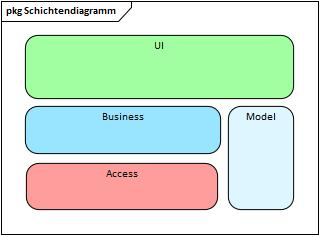
\includegraphics[width=\linewidth]{assets/images/layering}
		\end{center}
		\caption{GVS 2.0 Layering}
		\vspace{-20pt}
	\end{wrapfigure}
	
	In einer ersten Phase wird die bestehende Software auf Funktionsweise und Verbesserungspotential analysiert. Ebenfalls wird die umgesetzte Architektur kritisch beleuchtet. Da die Software \gls{hsr}-intern verwendet wird, sind Folgearbeiten nicht auszuschliessen. Es wird deshalb darauf geachtet, dass mit den gewonnenen Erkenntnissen eine Architektur designet wird, die einfach verständlich und erweiterbar ist. Zudem sollen zeitgemässe Softwareentwicklungs-Techniken angewendet werden. \\
	
	\noindent
	Das in die Jahre gekommene Java \gls{swing} GUI Toolkit wird im Rahmen dieser Studienarbeit mit dem offiziellen Nachfolger \gls{javafx} ersetzt. 
	
	\subsection*{Ergebnisse}
	In der Studienarbeit wurde ein vollständiger Ersatz für den GVS 1.0 entwickelt.\\
	Die Code Qualität konnte durch die Umsetzung einer klaren Schichtenarchitektur und zahlreichen Refactorings gesteigert werden. Dabei wurde ein besonderes Augenmerk auf das Einhalten des \gls{single-responsibility} und auf die Reduktion von dupliziertem Code gelegt. Somit konnten sämtliche Metrik-Noten verbessert werden.\\
	Eine Verbesserung der Usability wurde unter anderem durch ein modernes UI mit starken Farbkontrasten und eine automatisch skalierende und zentrierende Zeichenfläche erreicht. Zudem ist GVS 2.0 robuster gegenüber Programmierfehler in der User-Applikation. Bei auftretenden Exceptions springt ein Watchdog ein und kappt die Verbindung zwischen Client und Server.\\
	GVS 2.0 erweitert den bisherigen Funktionsumfang um einen Algorithmus für Trees, welcher fähig ist auch grosse Binary-Trees ansprechend und lesbar zu zeichnen sowie \glspl{n-ary} darzustellen.
	
	\subsection*{Ausblick}
	Das Projektteam ist vom praktischen Nutzen der Applikation überzeugt und wird sich deshalb in der Bachelorarbeit mit einer generischen Lösung zur Visualisierung von weiteren theoretischen Informatikkonzepten beschäftigen.
	
	\begin{figure}[h!]
		\centering
		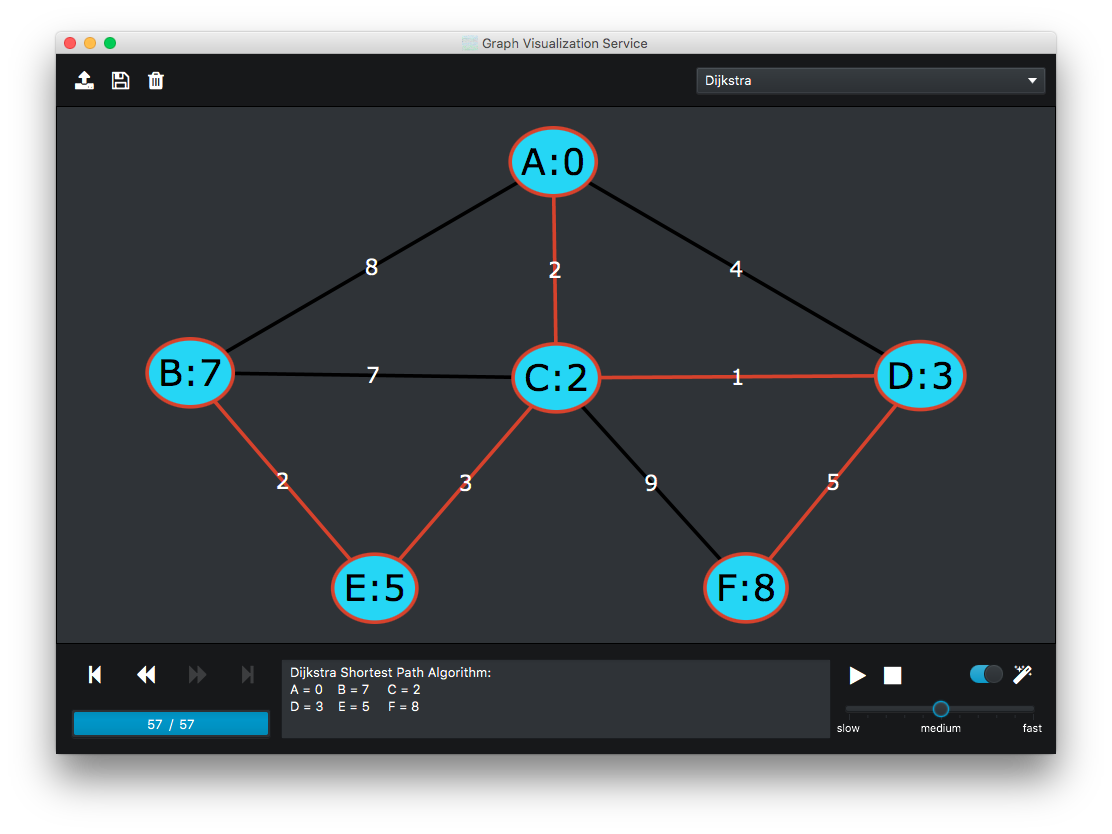
\includegraphics[width=0.6\linewidth]{assets/images/gvs-overview}
		\caption{Visualisierter Dijkstra Algorithmus im GVS UI 2.0}
		\label{fig:gvs-overview}
	\end{figure}
	
	
	\newpage
	
	\section*{Danksagungen}
	\thispagestyle{firststyle}
	
	Wir danken folgenden Personen für Ihre Unterstützung:
	
	\begin{itemize}
		\item Thomas Letsch für die Betreuung und Unterstützung während unserer Studienarbeit
		\item Prof. Olaf Zimmermann für die interessanten Gespräche während der Architekturphase
		\item Jessica Martin für die technische Unterstützung beim Logo Design
	\end{itemize}
	

	{
		\hypersetup{linkcolor=black}
		\tableofcontents
	}

	\newpage
	\pagenumbering{arabic}
	
	
	\chapter{Ausgangslage}
	
	\begin{table}[h!]
		\centering
		\begin{tabularx}{\linewidth}{l l X l}
			\toprule 
			Datum & Version & Änderungen & Autor \\
			\midrule
			28.09.17 & 1.0 & Grundgerüst erstellt & mwieland, mtrentini \\
			18.12.17 & 1.0 & Mehrwert ergänzt & mtrentini \\
			\bottomrule 
		\end{tabularx} 
		\caption{Versionshistory Ausgangslage} 
	\end{table}
	
	
	\section{Problembeschreibung}
	An der \gls{hsr} werden in den Modulen \textit{Algorithmen und Datenstrukturen 1} und \textit{Algorithmen und Datenstrukturen 2} die Funktionsweise von schwierig zu verstehenden Algorithmen unterrichtet. Zusätzlicher Bestandteil der Module ist das Erlernen der beiden Datenstrukturen \textit{Graph} und \textit{Tree}. Die Implementierung derartiger Algorithmen und Datenstrukturen ist oft mit grossem Aufwand verbunden. \\
	Die Software \gls{gvs} unterstützt Studenten beim Erlernen der beiden Datenstrukturen sowie der darauf anwendbaren Algorithmen. Damit sich die Studenten ausschliesslich auf das Erlernen der Algorithmen fokussieren können, bietet GVS eine Library, welche den Studenten repetitive Implementierungsarbeiten abnimmt. Der wichtigste Aspekt ist jedoch die Visualisierung der Arbeitsweise von Datenstrukturen und Algorithmen. So zeigt die Software zum Beispiel den schrittweisen Aufbau eines Baumes oder den Ablauf des Path Finding Algorithmus ''Dijkstra''. \\
	Die Software wurde 2005 bereits im Rahmen einer Bachelorarbeit umgesetzt. Der in die Jahre gekommene GVS 1.0 soll nun in einem Major-Upgrade aktualisiert werden.
	
	
	
	\section{Mehrwert}
	\gls{gvs} wird im Rahmen dieser Studienarbeit auf den neusten Stand der Technik gebracht und profitiert von neueren Java Features wie Generics und Lambdas sowie einer erweiterbaren Schichtenarchitektur. \\
	
	\noindent
	Für den Endbenutzer ändert sich hauptsächlich das User Interface. Dieses bekommt ein modernes und ansprechendes Design, besitzt intuitiven Zugriff auf vorhandene Features und ist durch die automatisch skalierende und zentrierende Zeichenfläche flexibler in der Darstellung von Graphen und Trees. Zudem hat die Applikation durch das Einführen eines Watchdogs (siehe \ref{sec:watchdog}) eine höhere Fehlertoleranz. \\
	
	\noindent
	Durch die Verbesserung der Code Qualität und die Einführung einer sauberen Schichten-Architektur, wird es zukünftigen Entwicklern leichter gemacht, die Applikation zu verstehen und zu erweitern.	
	
	%TODO: ausführen!!
	
	
	
	\chapter{Anforderungsspezifikation}
	
	\begin{table}[h!]
		\centering
		\begin{tabularx}{\linewidth}{l l X l}
			\toprule 
			Datum & Version & Änderungen & Autor \\
			\midrule
			17.10.17 & 1.0 & Sequenzdiagramme eingefügt & mtrentini \\
			18.10.17 & 1.1 & Stakeholder eingefügt & mwieland \\
			19.10.17 & 1.2 & Erkenntnisse: Stärken, Schwächen, Schlüsse beschrieben & mwieland \\
			\bottomrule 
		\end{tabularx} 
		\caption{Versionshistory Anforderungsspezifikation} 
	\end{table}
	
	
	
	\section{Anforderungen} \label{sec:functionalreq}
	Die Anforderungen werden massgeblich aus der offiziellen Aufgabenstellung entnommen. (siehe Anhang \ref{aufgabenstellung})
	
	\subsection{Funktionale Anforderungen}
	Die funktionalen Anforderungen werden vollständig von GVS 1.0 \cite{gvs1} übernommen. Der Funktionsumfang der Applikation soll nicht verändert werden. Sollten dennoch Anpassungen am Funktionsumfang nötig sein, werden diese mit dem Betreuer besprochen und in den Sitzungsprotokollen dokumentiert.
	
	\subsection{Nicht funktionale Anforderungen}
	
	\begin{enumerate}
		\item In der \gls{gvsui} Komponente muss das Framework Swing durch \gls{javafx} ersetzt werden.
		\item In der \gls{gvslib} Komponente muss die Java und .NET Library um Generics erweitert werden. 
		\item Punktuell müssen Verbesserungen vorgenommen werden.
	\end{enumerate}

	\noindent
	Eine genaue Definition der dritten Anforderung ist im Abschnitt Refactoring Ablauf (\ref{ssec:ablauf}) beschrieben.
	
	\section{Domainanalyse}
	In der Domainanalyse wird der GVS 1.0 untersucht. Die Erkenntnisse fliessen in die Designspezifikation ein.
		
	\subsection{Stakeholder} \label{ssec:stakeholder}
	Stakeholder repräsentieren Personen, die ein Interesse an der vorliegenden Software haben. Aus den funktionalen Anforderungen (\ref{sec:functionalreq}) von GVS 1.0 können drei relevant Stakeholder ermittelt werden. Während der Umsetzung wird überprüft, ob die Erwartungen der Stakeholder erfüllt werden können. Wegen der technischen Orientierung der vorliegenden Studienarbeit werden speziell die Ansprüche zukünftiger Entwickler berücksichtigt.
	
	\begin{table}[h!]
		\centering
		\begin{tabularx}{\linewidth}{l l X X}
			\toprule 
			\# & Rolle & Ziel/Intention & Erwartungshaltung \\
			\midrule
			1 & Student & Möchte GVS unkompliziert installieren und benutzen können. (Unter Zuhilfenahme der Installationsanleitung) & Möchte den zu visualisierenden Graphen/Tree ansprechend dargestellt bekommen. Ihm ist der Lerneffekt wichtig.  \\
			2 & Entwickler & Möchte GVS einfach erweitern können. & Sucht nach bekannten Software Pattern und klaren Software Schichten. Erwartet eine informative Architekturdokumentation. \\			
			3 & Dozent & Möchte GVS in seinem Unterricht einsetzen. & Erwartet eine intuitive Integration von GVS in bestehende Übungsaufgaben. \\
			\bottomrule 
		\end{tabularx} 
		\caption{Relevante Stakeholder} 
	\end{table}

	\subsection{Aktoren} \label{ssec:actors}
	Aktoren sind externe Einflussfaktoren die mit dem System interagieren. Im GVS 1.0 gibt es zwei Aktoren.
	
	\subsubsection{GVS User} \label{sssec:actor-user}
	Der GVS User interagiert mit dem \gls{gvsui} über das User Interface. Er kann die aktuelle Visualisierungs-Session per Knopfdruck auf das Filesystem speichern oder eine bestehende Session von dort laden. Wenn ein Graph visualisiert ist, kann er die Koordinaten der Vertices neu berechnen lassen.
	
	\subsubsection{GVS Lib} \label{sssec:actor-lib}
	Die \gls{gvslib} Komponente wird in das Software Projekt des GVS Users eingebunden. Sie sendet in \gls{xml} beschriebene Datenstrukturen über eine Socket Verbindung an das \gls{gvsui}. Die Daten werden vom \gls{gvsui} auf dem Access Layer empfangen und auf dem User Interface visualisiert.
	
	\subsection{Systemübersicht}
	Die Systemübersicht zeigt schematisch wie die beiden Aktoren (Siehe \ref{ssec:actors}) mit dem  die \gls{gvsui} interagieren.
	
	\begin{figure}[h!]
		\centering
		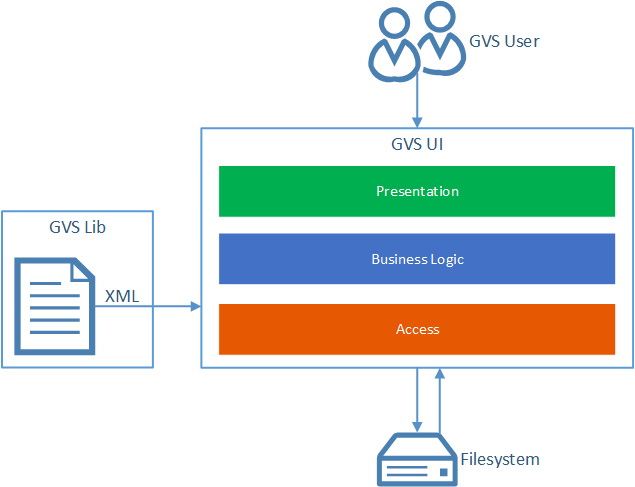
\includegraphics[width=0.5\linewidth]{assets/images/system_overview}
		\caption{GVS: Systemübersicht}
		\label{fig:gvs-systemuebersicht}
	\end{figure}
	
	\subsection{Klassendiagramm} \label{ssec:klassendiagramm-1}
	Das Klassendiagramm 1 (\textit{Klassendiagramm UI Analyse} im Anhang \ref{ch:class-diagram}) zeigt die wichtigsten Klassen von GVS 1.0. Im vorhergehenden Projekt wurden die Schichten zwar angedacht, sie widerspiegeln sich aber kaum im Package Design. Um den Überblick zu verbessern, sind die Klassen in diesem Diagramm den entsprechenden Schichten zugewiesen. Dies erhöht die Verständlichkeit der Problemdomäne und vereinfacht den Übergang in die neue Schichtenarchitektur von GVS 2.0. Eine genaue Analyse der GVS 1.0 Klassen ist dem Abschnitt \ref{sec:erkenntnisse} zu entnehmen. 
		
	\subsection{Sequenzdiagramme} \label{ssec:sequence-1}
	Um schwierig zu verstehende Systemabläufe zu abstrahieren, werden Systemdiagramme erstellt. Sie zeigen die wichtigsten Abläufe in GVS 1.0.
	
	\subsubsection{Verbindungsaufbau}
	Das Sequenzdiagramm	\ref{fig:sd-verbindungsaufbau} zeigt den Verbindungsaufbau über den \textit{SocketServer} beim Starten der Applikation. Der Start einer \textit{ServerConnectionXML} führt zu einem Locking mit Hilfe des \textit{ConnectionMonitors}. Dieses Locking verhindert, dass mehr als eine \gls{gvslib} gleichzeitig mit einem \gls{gvsui} kommuniziert. Nach dem Empfangen der Daten aus dem Socket, erstellt der \textit{ModelBuilder} einen Graphen oder Tree als Domain-Objekt. Dieser Ablauf ist auf dem Sequenzdiagramm \textbf{ModelBuilder} (siehe \ref{sssec:modelbuilder}) ersichtlich.
	\begin{figure}[h!]
		\centering
		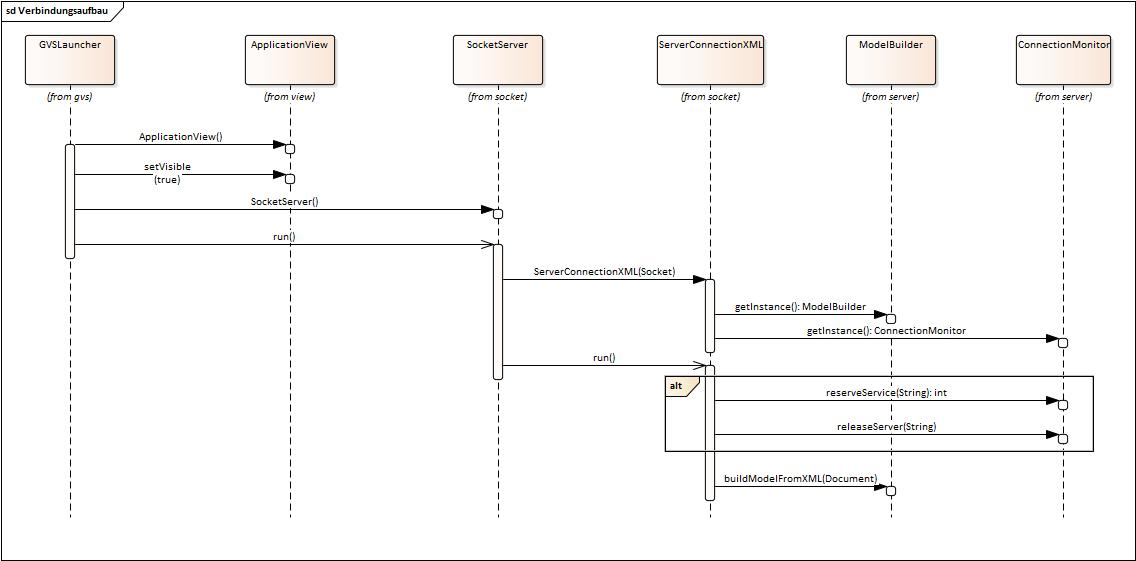
\includegraphics[width=\linewidth]{assets/images/verbindungsaufbau}
		\caption{Sequenzdiagramm: Verbindungsaufbau}
		\label{fig:sd-verbindungsaufbau}
	\end{figure}

	\subsubsection{ModelBuilder} 	\label{sssec:modelbuilder}
	Wie im Sequenzdiagramm \ref{fig:sd-modelbuilder} parsed der \textit{ModelBuilder} aus den empfangenen \gls{xml} Dokumenten das entsprechende Domain-Objekt. Dabei wird zwischen Graphen und Trees unterschieden. Nach Fertigstellung des Parse-Vorgangs, wird das Model an den entsprechenden \textit{SessionController} übergeben. Der weitere Ablauf befindet sich im separaten Sequenzdiagramm \textbf{GraphSessionController} (siehe \ref{sssec:sessioncontroller})
	\begin{figure}[h!]
		\centering
		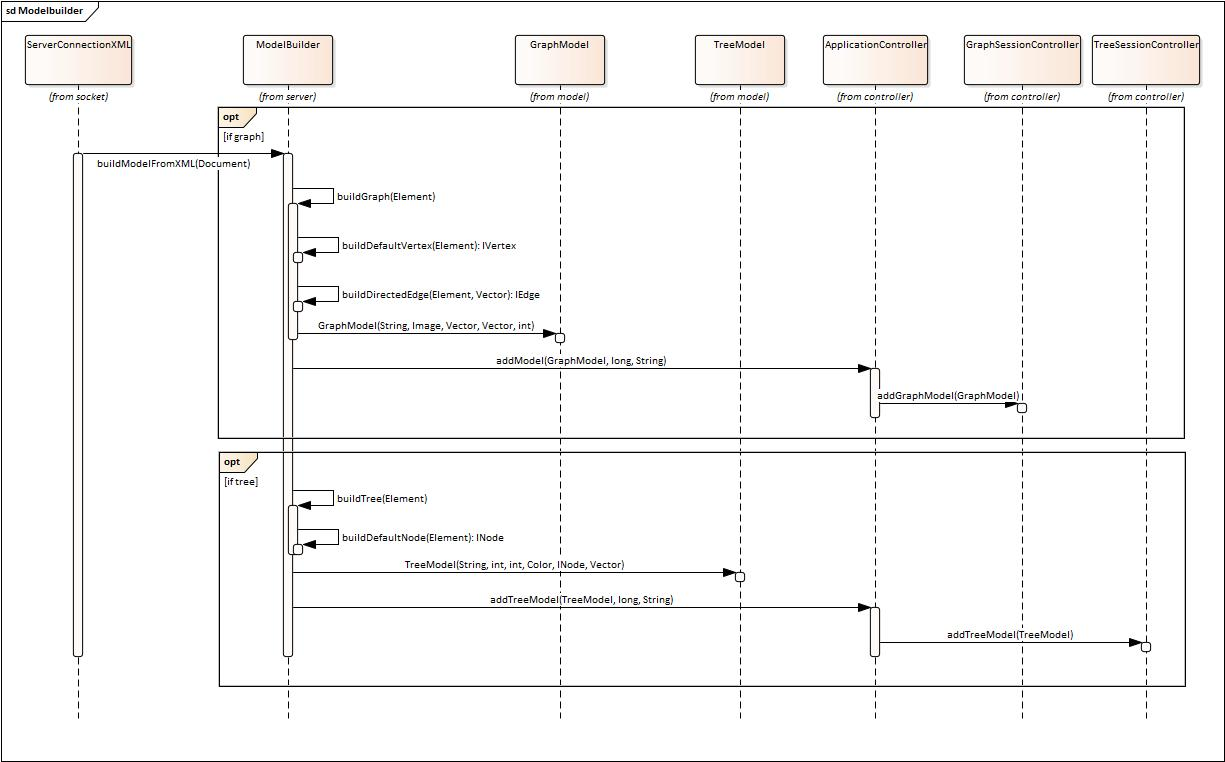
\includegraphics[width=\linewidth]{assets/images/modelbuilder}
		\caption{Sequenzdiagramm: ModelBuilder}
		\label{fig:sd-modelbuilder}
	\end{figure}

	\subsubsection{ApplicationView: Load \& Save Session} \label{sssec:appView}
	Der Programmablauf beim Laden und Speichern einer Session ist im Sequenzdiagramm \ref{fig:sd-applicationview} dargestellt. \\
	Wenn ein User eine Session lädt, wird das entsprechende \gls{xml} vom \textit{Persistor} geparsed. Je nach Bedarf wird ein Vector aus Graphen oder Trees erstellt. Dieser Vector wird an den \textit{SessionController} übergeben. Der Ablauf innerhalb des \textit{SessionController}s ist im separaten Sequenzdiagramm \textbf{GraphSessionController} (siehe \ref{sssec:sessioncontroller}) dargestellt. \\
	Nachdem die Session erstellt wurde, wird die \textit{ApplicationView} per Observer-Beziehung (siehe Glossar: \gls{observer}) notifiziert. Sie stellt darauf die neue Session im \gls{gvsui} dar.\\
	Auffällig an der Klasse \textit{ApplicationView} ist, dass sie im Constructor einen \textit{Persistor} instanziert. Diese Instanz wird jedoch nicht direkt in der ApplicationView verwendet, sondern wird als Argument an den \textit{ApplicationController} geschickt, welcher dann mit dem Persistor Sessions speichert und lädt. In der Analyse des Projektteams ist unklar geblieben, wieso die Instanzierung des \textit{Persistor}s nicht direkt im \textit{ApplicationController} passiert.
	\begin{figure}[h!]
		\centering
		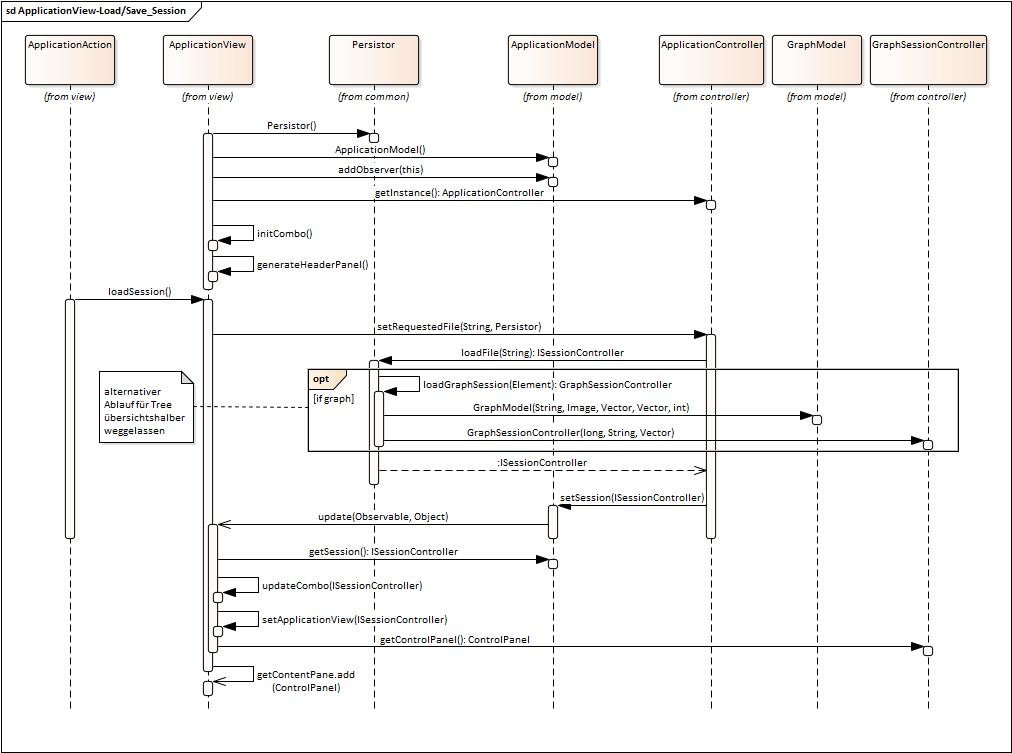
\includegraphics[width=\linewidth]{assets/images/application_view}
		\caption{Sequenzdiagramm: ApplicationView}
		\label{fig:sd-applicationview}
	\end{figure}

	\clearpage

	\subsubsection{GraphSessionController} \label{sssec:sessioncontroller}
	Wie das Sequenzdiagramm \ref{fig:sd-graphsessioncontroller} zeigt, wird der \textit{GraphSessionController} vom \textit{ModelBuilder} und vom \textit{Persistor} angestossen, wenn ein oder mehrere neue Graphen geparsed wurden. Der \textit{GraphSessionController} ist dafür zuständig diese Graphen in eine neue oder bestehende Session einzufügen. Dabei unterscheidet sich der Programmablauf kaum. Der besseren Übersicht halber ist nur der Fall ''ein einzelner neuer Graph wurde empfangen'' abgebildet.\\
	Für Graphen die keine fix positionierte Vertices haben, wird in einem weiteren Schritt der \textit{LayoutController} aufgerufen. Dieser steuert die Funktionalität der Physics-Engine. Die Physics-Engine berechnet die Koordinaten von Vertices mittels anziehenden und abstossenden Kräften. (siehe \gls{forcedirecteddrawing}) Der \textit{GraphSessionController} wird  per Observer-Beziehung (siehe Glossar: \gls{observer}) informiert, sobald die Physics-Engine die Berechnung der Positionen abgeschlossen hat.\\
	Der \textit{GraphSessionController} setzt den neuen Graphen als aktuellen Graphen auf dem \textit{VisualizationGraphModel}. Dieses informiert per Observer-Beziehung (siehe Glossar: \gls{observer}) das \textit{VisualiztionGraphPanel}, welches die für die Darstellung benötigten Vertex und Edge Komponenten erstellt.
	\begin{figure}[h!]
		\centering
		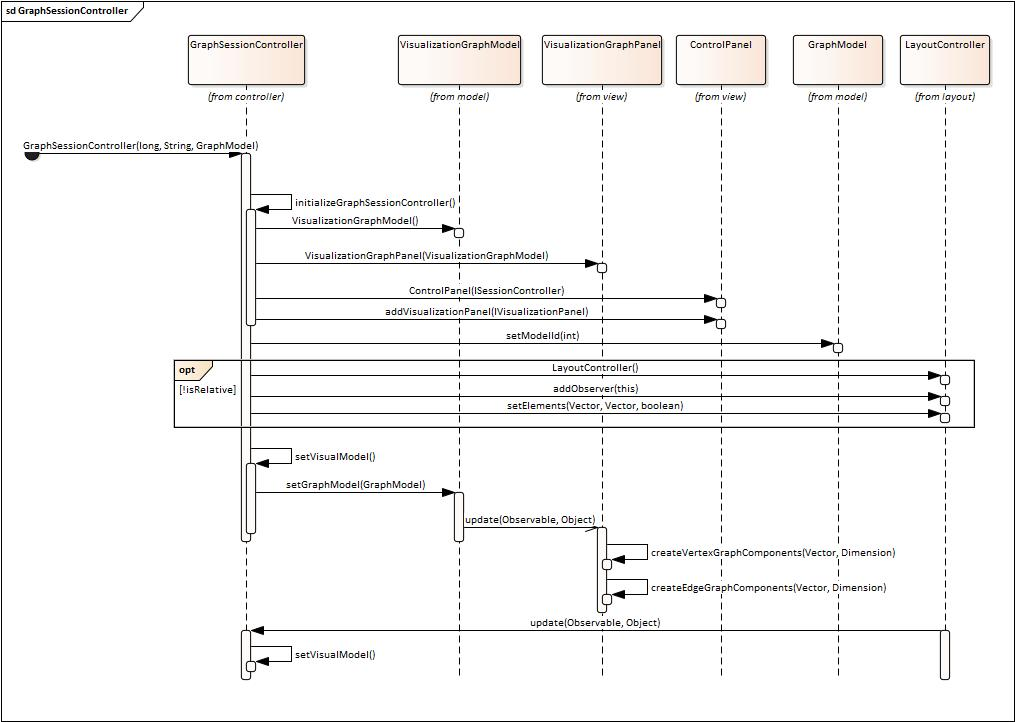
\includegraphics[width=\linewidth]{assets/images/graph_session_controller}
		\caption{Sequenzdiagramm: GraphSessionController}
		\label{fig:sd-graphsessioncontroller}
	\end{figure}

	\clearpage
	
	\subsection{Erkenntnisse} \label{sec:erkenntnisse}
	Die aus der Analysephase gewonnenen Erkenntnisse fliessen in die Designspezifikation ein.
		
	\begin{description}
	\item[Layering] \hfill \\
	Dem Projektplan GVS 1.0 \cite{gvs1} kann eine Schichtenarchitektur bestehend aus zwei Schichten entnommen werden. Die Schichten widerspiegeln sich aber nicht im Package Design. Gut erkennbar ist das Server Interface, dass die Visualisierung vom Socket Server trennt. GUI spezifische Imports ziehen sich durch mehrere Layer.
	
	\item[Swing/AWT Imports im Business Layer] \hfill \\ \label{sssec:swing-business}
	Im Business Layer gibt es diverse Imports der UI Frameworks \gls{swing} rsp. \gls{awt}. Dies erschwert einen einfachen Austausch des eingesetzten UI Frameworks.
	
	\item[Tangles] \hfill \\
	Zwischen dem Presentation und Business Layer existieren \glspl{tangle}. Dies verhindert einen einfachen Austausch des Presentation Layers. 
	
	\item[Magic Numbers] \hfill \\
	Viele Konstanten sind ungenügend beschrieben. Der Zweck von vielen Zahlen ist daher nur schwer nachvollziehbar.
	
	\item[Namenskonvention] \hfill \\
	Es gibt keine durchgehende Namenskonvention. Den Variablen fehlt es oft an Informationsgehalt. Ebenfalls sind veränderbare Variablen in Grossbuchstaben geschrieben, was per Konvention \cite{jls-naming} den Konstanten vorbehalten ist.
	
	\item[Temporary Fields] \hfill \\
	Viele Klassen arbeiten exzessiv mit Klassenvariablen, die in diversen Methoden gesetzt und gelesen werden. Des Weiteren werden die Klassenvariablen von Funktionsparameter und lokalen Variablen überdeckt.   
	
	\item[Duplicated Code] \hfill \\
	Klassen wie der \textit{ModelBuilder} und \textit{Persistor} übernehmen sehr ähnliche Aufgaben.
	
	\item[Long Classes] \hfill \\
	Einige Klassen überschreiten die Obergrenze von 250 Zeilen Code/Klasse. Dies hebt den Verdacht, dass die Klassen mehr als eine Aufgabe erledigen und somit das ''Single Responsibility Principle'' verletzen.
	
	\item[Keine Unit Tests] \hfill \\
	Im GVS 1.0 wurden keine Unit Tests geschrieben. Die Klassen sind sehr schwer testbar, da kein \gls{di} umgesetzt wurde.
	
	\item[JavaDoc] \hfill \\
	Das Verhalten von Klassen ist nicht durchgehend dokumentiert.  Ebenfalls fehlt es bei einigen Kommentaren an Aussagekraft.
	
	\end{description}	

		
	\chapter{Architektur und Designspezifikation}
	\label{ch:design-spec}
	
	\begin{table}[h!]
		\centering
		\begin{tabularx}{\linewidth}{l l X l}
			\toprule 
			Datum & Version & Änderungen & Autor \\
			\midrule
			13.10.17 & 1.0 & MVVM Konzept geschrieben & mwieland \\
			19.10.17 & 1.1 & Refactoring Konzept erstellt & mtrentini \\
			20.10.17 & 1.1 & Klassendiagramm 2.0 & mtrentini, mwieland \\
			\bottomrule 
		\end{tabularx} 
		\caption{Versionshistory Architektur und Designspezifikation} 
	\end{table}
	
	
	
	\section{Klassendiagramm} \label{sec:class-diagram}
	Das Klassendiagramm 2 \textit{''Klassendiagramm Entwurf''} im Anhang \ref{ch:class-diagram} orientiert sich stark an der Vorgängerversion des GVS 1.0. (Siehe \ref{ssec:klassendiagramm-1}). Mit dem Ziel möglichst viel Code wiederzuverwenden, wird der Access und Business Layer mehrheitlich beibehalten. Der Presentation Layer wird vollständig durch die neu eingeführte \gls{mvvm} Struktur ersetzt (Siehe \ref{sssec:mvvm}).
	
	\clearpage
	
	\section{Schichtenstruktur} \label{ssec:layer-architecture}
	
	\subsection{Presentation Layer}
	Der Presentation Layer wird von der restlichen Anwendung entkoppelt. Damit kann das eingesetzte UI Framework (z.B \gls{javafx}) leicht ersetzt werden. Der Presentation Layer ist nach dem \gls{mvvm} Prinzip organisiert.
	
	\subsubsection{Model-View-ViewModel} \label{sssec:mvvm}
	\gls{mvvm} dient der Trennung zwischen dem User Interface und der Anzeigelogik. MVVM ist eine Konkretisierung des verbreiteten \gls{mvc} Pattern und setzt stark auf Databindings. Es wurde von Microsoft für das \gls{wpf} Framework entwickelt und wird auch in modernen \gls{javafx} Applikation eingesetzt.
	
	\begin{figure}[h!]
		\centering
		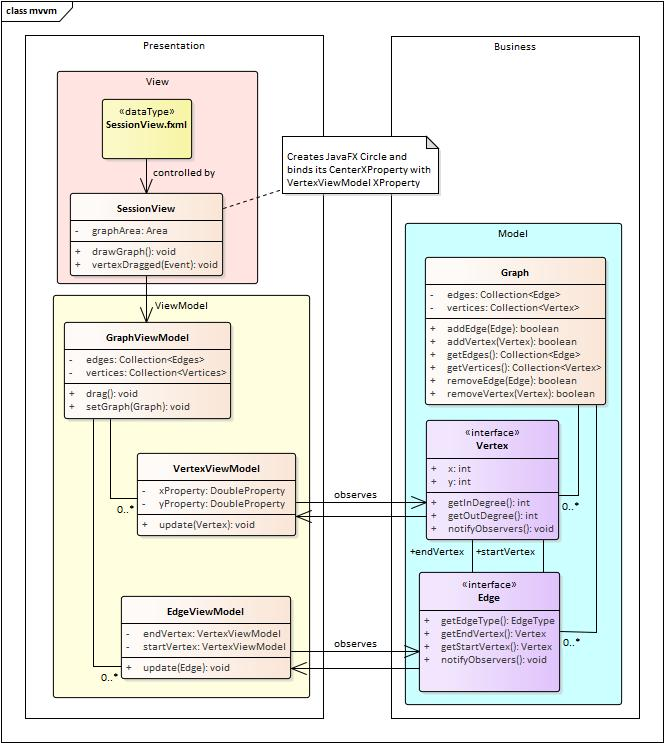
\includegraphics[width=0.7\linewidth]{assets/images/mvvm_concept}
		\caption[MVVM Konzept]{Übersicht Model View ViewModel}
		\label{fig:mvvmconcept}
	\end{figure}
	
	\paragraph{Model}
	Das \textit{Model} enthält reine Datenklassen ohne nennenswerte Logik. (siehe \gls{pojo}) Das \textit{Model} wird in den Business Layer verschoben, damit das UI Framework einfach ausgewechselt werden kann. Werden die Werte im Model geändert, wird das \textit{ViewModel} über eine Observer Beziehung (\gls{observer}) benachrichtigt. Dies entspricht nicht dem klassischen \gls{mvvm} Konzept, wird jedoch benötigt, damit die View entsprechend aktualisiert wird, wenn z.B die Vertex-Koordinaten neu berechnet werden.
	
	\paragraph{View}
	Die \textit{View} stellt den UI Zustand des \textit{ViewModels} dar. Sie setzt sich aus einer Controller Klasse sowie einer deklarativen \gls{fxml} Datei zusammen. Die View hält eine Instanz des ViewModels und leitet die eingehenden Anfragen direkt an dieses weiter. Mit der Databinding-API wird eine bidirektionale Kommunikation zwischen \textit{View} und \textit{ViewModel} sichergestellt. 
	
	\paragraph{ViewModel}
	Das \textit{ViewModel} kennt die View nicht. Es hat somit keine Abhängigkeiten zu konkreten Anzeige-Elementen. Dies hat den grossen Vorteil, dass die gesamte UI Logik im \textit{ViewModel} gekapselt ist und somit sehr gut testbar ist. Das ViewModel enthält \gls{javafx} spezifische Properties, die für das bidirektionale Binding zwischen UI Komponenten und Code Behind nötig sind \cite{javafxbook}.
	
	\subsection{Business Layer}
	Im Business Layer liegt die eigentliche Logik. Er enthält keine \gls{javafx} Komponenten, weshalb das eingesetzte UI Framework ohne weiteres ausgewechselt werden kann. 
	
	\subsection{Access Layer}
	Der Access Layer enthält Klassen für den Zugriff auf den Socket Server, sowie das File System. Es Ist für das Parsen von eingehenden XML Files zuständig und für deren Umwandlung in Domainobjekte.



	\section{Refactoring Konzept} \label{sec:refactoring-concept}
	Das Refactoring des GVS 1.0 soll organisiert durchgeführt werden. Dazu werden die notwendigen Schritte priorisiert aufgelistet.
		
	\subsection{Ablauf}\label{ssec:ablauf}
	\begin{enumerate}
		\item Der Presentation Layer wird ersetzt. Dabei wird \gls{swing} durch \gls{javafx} ersetzt. Mehr Details finden sich in der Migrations Liste (\ref{ch:migration-list}) sowie im Klassendiagramm von GVS 2.0 (\ref{sec:class-diagram})
		\item Die GVS 1.0 Library wird um Generics erweitert. Dies betrifft die Java-, sowie die .NET Library.
		\item Eine klare Schichtenarchitektur (\ref{ssec:layer-architecture}) wird eingeführt. Besonders wichtig ist dabei, das Entfernen von \glspl{tangle}.
		\item Duplicated Code und weitere Code Smells sollen entfernt werden. Ein besonderes Augenmerk wird auf ein konsequentes Naming, das \gls{dry} Konzept sowie das \gls{single-responsibility} für Klassen und Methoden gelegt.
	\end{enumerate}

	\subsection{Migrations Liste}
	\label{ssec:class-refactroing-list}
	Die Migrations Liste im Anhang (siehe \ref{ch:migration-list}) zeigt, welche Klassen aus GVS 1.0 übernommen werden und welche Klassen in welcher Art und Weise verändert oder neu erstellt werden.

	
	\chapter{Umsetzung} \label{ch:umsetzung}
		
	\begin{table}[h!]
	\centering
	\begin{tabularx}{\linewidth}{l l X l}
		\toprule 
		Datum & Version & Änderungen & Autor \\
		\midrule
		28.09.17 & 1.0 & Dokument erstellt, Logo beschrieben & mwieland \\
		06.12.17 & 1.1 & Gerichtete Kanten beschrieben & mtrentini \\
		07.12.17 & 1.2 & TreeLayouter beschrieben & mtrentini \\
		08.12.17 & 1.3 & GraphLayouter beschrieben & mwieland \\
		08.12.17 & 1.4 & Multithreading beschrieben & mwieland \\
		08.12.17 & 1.5 & Klassendiagramm GVS 2.0 & mtrentini \\
		08.12.17 & 1.6 & Presentation Layer beschrieben & mwieland \\
		10.12.17 & 1.7 & Client Library Update beschrieben & mwieland \\
		11.12.17 & 1.8 & Sequenzdiagramme beschrieben & mtrentini \\
		14.12.17 & 1.9 & Graph \& Tree Verschmelzung beschrieben & mtrentini \\
		17.12.17 & 1.10 & Watchdog beschrieben & mtrentini \\
		\bottomrule 
	\end{tabularx} 
	\caption{Versionshistory Umsetzung} 
	\end{table}



	\section{Umgesetzte Architektur}
	
	\subsection{Klassendiagramm}
	Das \textit{''Klassendiagramm UI Umsetzung''} im Anhang \ref{ch:class-diagram} zeigt einen Überblick über die wichtigsten Klassen in GVS 2.0 sowie die umgesetzte Schichtenarchitektur (siehe \ref{ssec:layer-architecture}). Durch den Einsatz des \gls{mvvm} Pattern ist der Presentation Layer in sich gekapselt. Im Gegensatz zum GVS 1.0 werden ausserhalb des Presentation Layers keine UI spezifischen Klassen verwendet. Dies ermöglicht einen Austausch des verwendeten UI Frameworks.
	

	\noindent
	Die folgende Aufzählung (\ref{desc:architecture-changes}) zeigt die wichtigsten Änderungen zum Klassendiagramm aus der Entwurfsphase auf. (siehe Anhang \ref{ch:class-diagram}) Ansonsten widerspiegelt GVS 2.0 die angedachte Architektur und Klassenhierarchie.
	
	\begin{description} \label{desc:architecture-changes}
		\item[GvsXmlReader \& ClientConnection ] \hfill \\ Diese Klassen entstanden durch ein Refactoring der GVS 1.0 Klasse \textit{ServerConnectionXML}. Die Trennung dieser Klasse führt dazu, dass das \gls{single-responsibility} eingehalten wird. 
		\item[Watchdog] \hfill \\ Behebt das Problem, dass beim Absturz eines Clients die Server Komponenten für andere Clients nicht wieder freigegeben wird. Dies erleichtert das Usability für den Benutzer sehr. Mehr dazu in Abschnitt \ref{sec:watchdog}
		\item[SessionType] \hfill \\ Trees und Graphen werden völlig unterschiedlich gelayoutet. Dennoch werden die gleichen Klassen für die Darstellung im Presentation Layer verwendet. Durch das \gls{type-object} kann trotzdem ein spezifischer Layouting Algorithmus für jede Datenstruktur eingesetzt werden.
		\item[TreeVertex \& LeafVertex] \hfill \\ 
		In der Designphase wurde das Zusammenführen von Graphen und Trees angedacht. In der Realisierung hat sich aber gezeigt, dass einerseits die Layouter sowie infolgedessen auch die Vertices unterschieden werden müssen. (siehe \ref{graph-vs-tree}) Für den Tree Layouter (\ref{sec:treelayouter}) wird neben dem \textit{TreeVertex} auch ein \textit{LeafVertex} benötigt.  Blattknoten dienen als Platzhalter die im UI nicht dargestellt werden. Sie vereinfachen die Berechnung des Tree Layouts aber stark.
	\end{description}

	\subsection{Layering} \label{ssec:layering}
	Der GVS 2.0 ist in drei horizontale Layer unterteilt.
	
	\begin{figure}[h!]
		\centering
		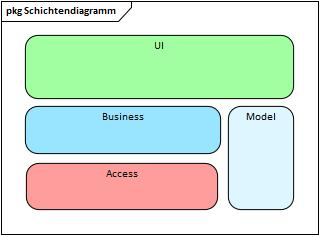
\includegraphics[width=0.5\linewidth]{assets/images/layering}
		\caption{GVS 2.0 Layering}
		\label{fig:layering}
	\end{figure}
	
	\noindent
	Die Zugriffe verlaufen durchgehend von höheren Schichten zu tieferen. Sämtliche \glspl{tangle} werden mit dem \gls{observer} aufgelöst. Einzige Ausnahme bildet das \textit{Model} Package, dass seitlich am \textit{Business} und \textit{Access} Layer positioniert ist. \\
	\noindent
	Das Strukturanalyse Tool markiert die Zugriffe zwischen \textit{Model} und \textit{Business} leider auch als Tangle (rot). Diese stellen jedoch kein Problem dar, da sich die beiden Packages logisch auf der selben Ebene befinden. Zur besseren Veranschaulichung dient das \textit{''Klassendiagramm UI Umsetzung''} im Anhang \ref{ch:class-diagram}.
	
	\begin{figure}[h!]
		\centering
		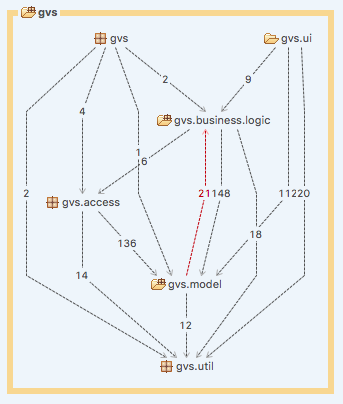
\includegraphics[width=0.4\linewidth]{assets/images/structure-gvs2}
		\caption{GVS 2.0 Package Struktur}
		\label{fig:structure-gvs2}
	\end{figure}
	
	
	\subsection{Sequenzdiagramme}
	Während der Analyse-Phase dieses Projekts wurden die Programmabläufe in GVS 1.0 untersucht (siehe \ref{ssec:sequence-1}). Um Änderungen im Programmablauf aufzuzeigen, finden sich in diesem Kapitel neue Sequenzdiagramme, die die selben Abläufe in GVS 2.0 abbilden. 
	
	\subsubsection{Verbindungsaufbau}
	Abbildung \ref{fig:sd-verbindungsaufbau-2} zeigt den Start der GVS 2.0 Applikation über die \textit{GVSApplication} sowie das Empfangen von Daten über die Socket. Nicht ersichtlich ist im Diagramm, dass GVS 2.0 an vielen Orten auf \gls{di} setzt (siehe \ref{DI}). Zum Beispiel werden die vier Klassen \textit{Watchdog},  \textit{ConnectionMonitor},  \textit{GvsXmlReader} und  \textit{ModelBuilder} (rechts im Diagramm) in den Constructor der  \textit{ClientConnection} ''injected''.
	
	\noindent
	Details zu den genauen Änderungen gegenüber GVS 1.0 finden sich im Abschnitt \ref{desc:architecture-changes}.

	\begin{figure}[h!]
		\centering
		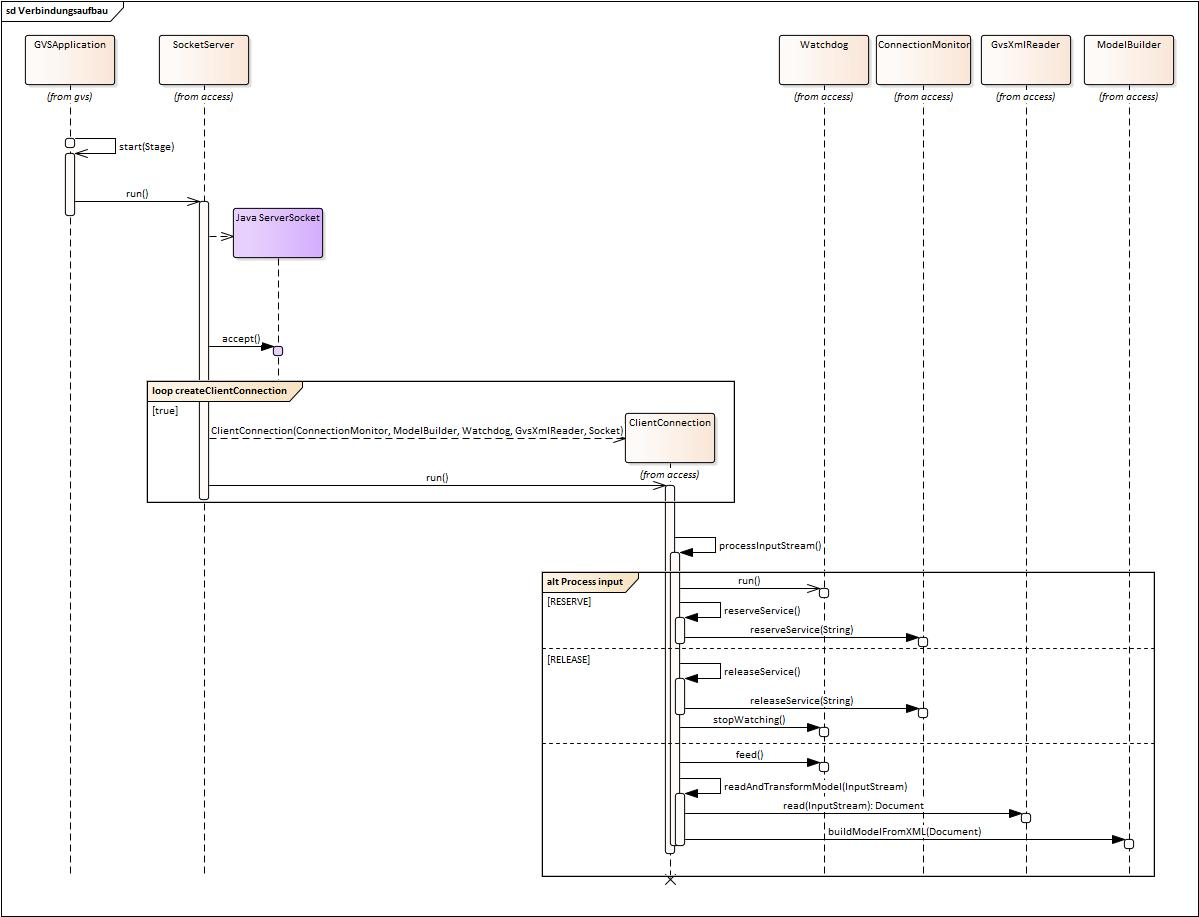
\includegraphics[width=\linewidth]{assets/images/sequence_Verbindungsaufbau}
		\caption{Sequenzdiagramm: Verbindungsaufbau}
		\label{fig:sd-verbindungsaufbau-2}
	\end{figure}

	\clearpage
	
	\subsubsection{ModelBuilder}
	Das Sequenzdiagramm in Abbildung \ref{fig:sd-modelbuilder-2} zeigt, wie aus einem empfangenen XML File \glspl{pojo} des Business Layers erstellt werden. Sehr gut erkennbar ist, dass im Vergleich zu GVS 1.0 die Trennung zwischen Graph und Tree viel weniger ausgeprägt ist, um \textit{duplicated Code} zu vermeiden (siehe \ref{graph-vs-tree}).
	\begin{figure}[h!]
		\centering
		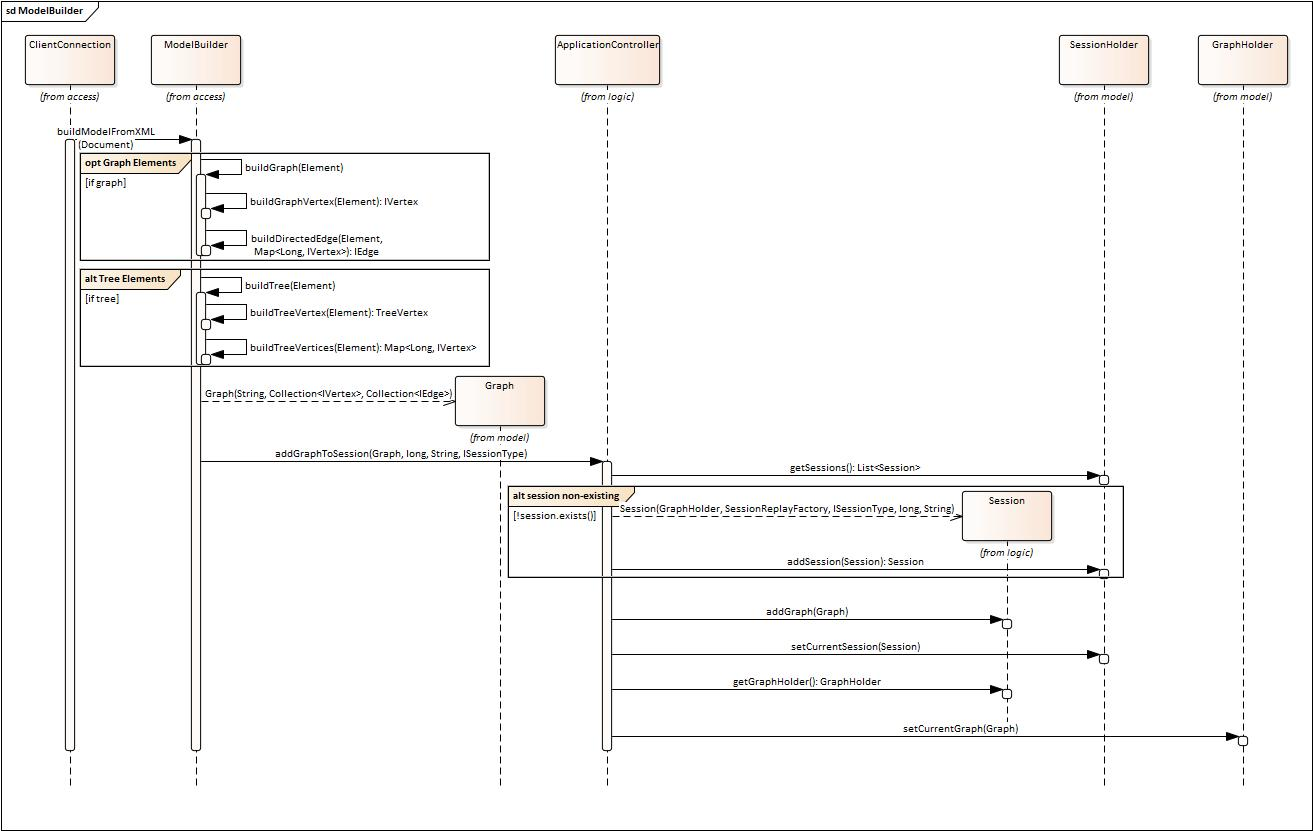
\includegraphics[width=\linewidth]{assets/images/sequence_ModelBuilder}
		\caption{Sequenzdiagramm: ModelBuilder}
		\label{fig:sd-modelbuilder-2}
	\end{figure}	

	\subsubsection{Load \& Save Session}
	Ein User von GVS 2.0 hat die Möglichkeit Sessions zu speichern und vorherige Sessions zu laden. Was sich dabei hinter den Kulissen abspielt, zeigt Abbildung \ref{fig:sd-load_save_session-2}. Die links eingezeichnete blaue Klasse \textit{JavaFX} widerspiegelt UI Events, welche per \textit{EventHandler} an die \textit{AppView} weitergeleitet werden.
	
	Durch die komplette Ersetzung des Presentation Layers sowie einer klareren Trennung der verschiedenen Schichten unterscheidet sich dieses Sequenzdiagramm stark vom entsprechenden Pendant in GVS 1.0 (\ref{fig:sd-applicationview}). Sie decken jedoch beide die gleichen Use Cases ab.
	
	\begin{figure}[h!]
		\centering
		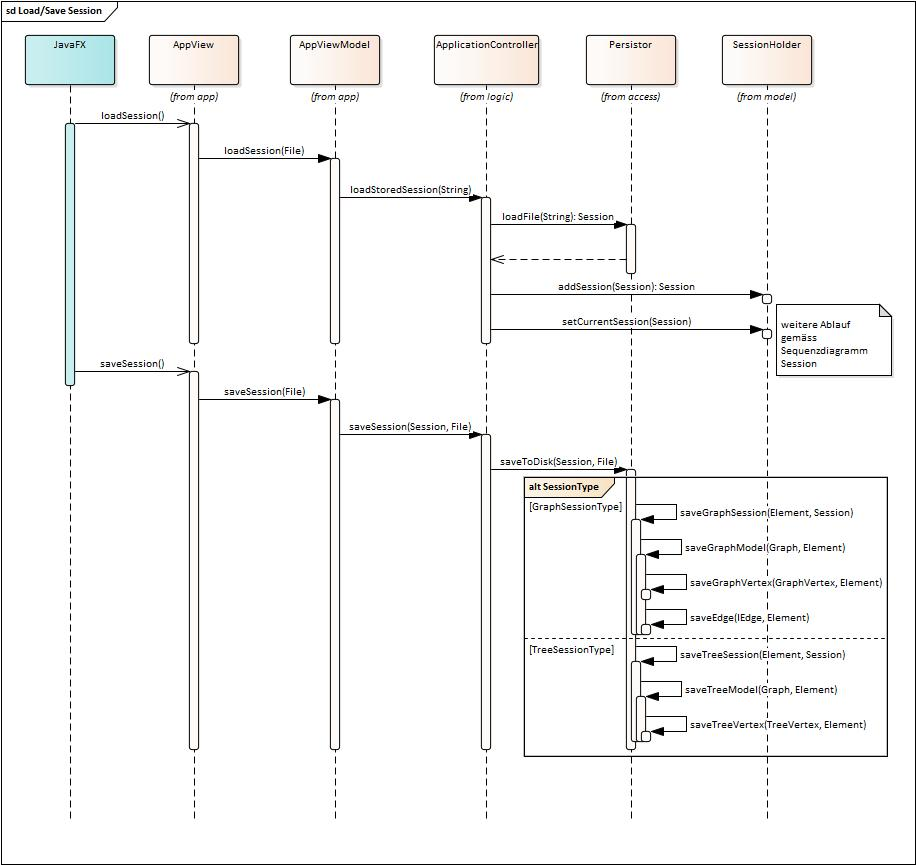
\includegraphics[width=\linewidth]{assets/images/sequence_LoadSave_Session}
		\caption{Sequenzdiagramm: Load \& Save Session}
		\label{fig:sd-load_save_session-2}
	\end{figure}
	
	\clearpage
	
	\subsubsection{Session}	
	Auch in Abbildung \ref{fig:sd-session-2} zeigen sich die Änderungen im Presentation Layer und die strukturellen Änderungen an der gesamten Applikation stark. So ist nicht auf den ersten Blick ersichtlich, dass Abbildung \ref{fig:sd-graphsessioncontroller} und Abbildung \ref{fig:sd-session-2} die gleiche Programmlogik aufzeigen, nämlich wie \glspl{pojo} des Business Layers an den Presentation Layer gelangen und auf dem UI dargestellt werden.
	
	\begin{figure}[h!]
		\centering
		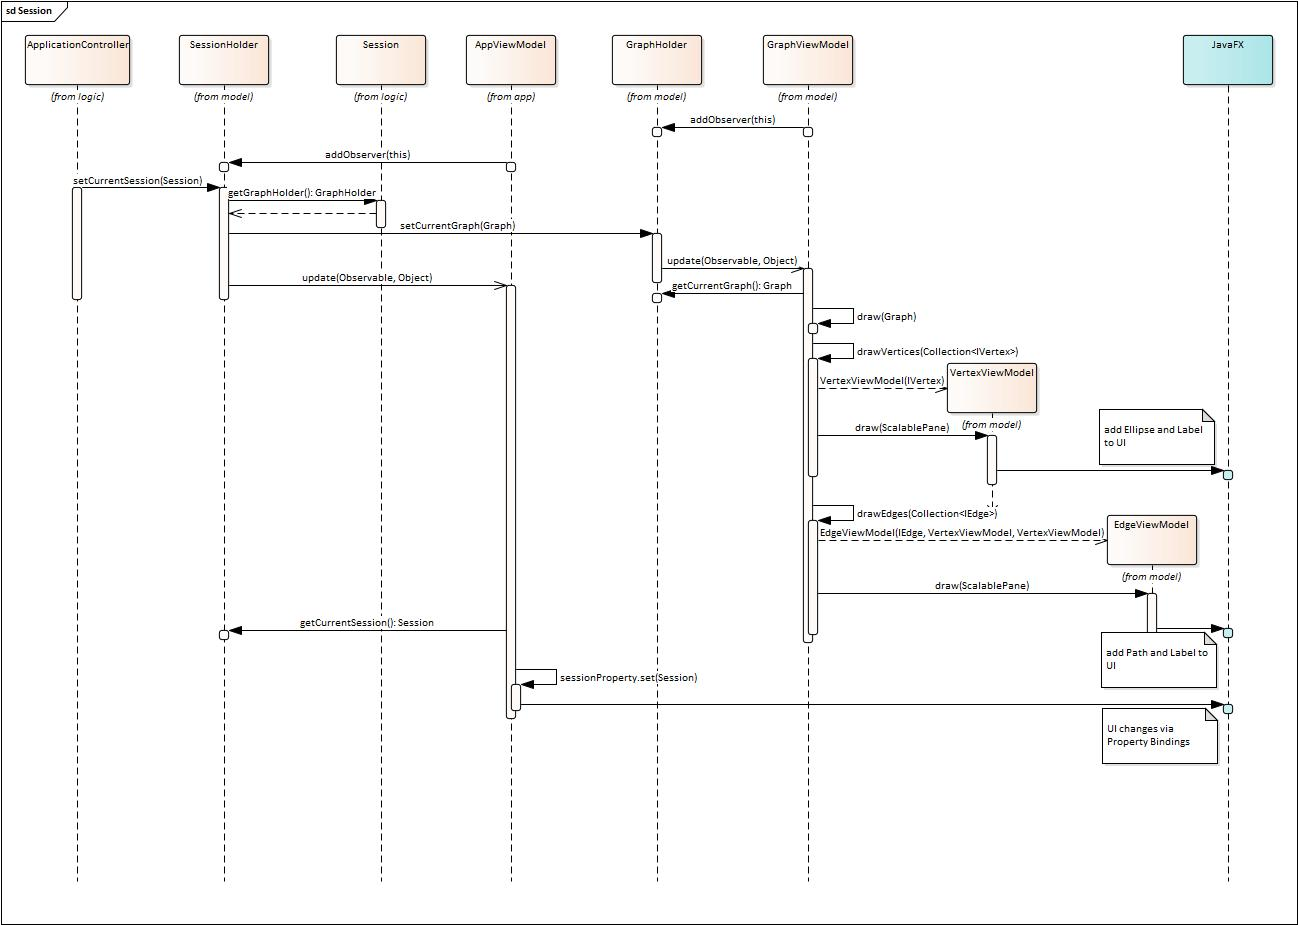
\includegraphics[width=\linewidth]{assets/images/sequence_Session}
		\caption{Sequenzdiagramm: Session}
		\label{fig:sd-session-2}
	\end{figure}

	\clearpage


	\section{Multithreading} \label{sec:threading}
	Um die Benutzeroberfläche reaktiv zu halten und gleichzeitig auf Datenübertragungen von der Client Lib zu reagieren werden mehrere Threads benötigt. Daher müssen Synchronisationspunkte eingerichtet werden, damit typische Gefahren der Nebenläufigkeit (z.B Race Conditions) nicht auftreten können. Im GVS 2.0 sind folgende Klassen als eigenständige Threads konzipiert.
	
	\subsection{Nebenläufige Klassen}
	Tabelle \ref{tbl:concurrent-classes} zeigt sämtliche nebenläufige Klassen des GVS 2.0.
	
	\begin{table}[h!]
		\centering
		\begin{tabularx}{\linewidth}{l X X}
			\toprule 
			Klasse & Beschreibung & Lebensdauer \\
			\midrule
			\textit{GVSApplication} & Läuft im Java Main Thread. Startet den \gls{javafx} UI Thread sowie den SocketServer Thread & Programmstart bis App Terminierung. \\
			UI Klassen & Alle UI Klassen laufen im JavaFX Thread & Programmstart bis App Terminierung \\
			\textit{SocketServer} & Startet einen \textit{SocketServer} auf einen konfigurierbaren Port und erstellt \textit{ClientConnection} Instanzen für jede eingehende Anfrage. & Programmstart bis App Terminierung. \\
			\textit{ClientConnection} & Interpretiert mit Hilfe des \textit{GvsXmlReaders} die eingehende Verbindung und leitet die XML Daten an den ModelBuilder weiter & Während einer Client Verbindung \\
			\textit{Watchdog} & Ermöglicht, dass ein Client den Server nur so lange reserviert wie auch Daten übertragen werden & Während einer Client Verbindung \\
			\textit{AreaTicker} & Representiert einen Layouting Pulse. Definiert wie oft die View während dem Layouting eines Graphen aktualisiert wird. & Während dem Layout Prozess eines Graphen \\
			\textit{SessionReplay} & Gibt Graph Snapshots in einem konfigurierbaren Intervall wieder & Solange die Session existiert \\
			\bottomrule 
		\end{tabularx} 
		\caption{Übersicht nebenläufige Klassen} 
		\label{tbl:concurrent-classes}
	\end{table}
	
	\subsection{Synchronisationspunkte}
	
	Die nebenläufigen Klassen werden von speziellen Synchronisationspunkten serialisiert, die in Tabelle \ref{tbl:sync-pt} aufgelistet sind. Die Synchronisationspunkte werden von Guice \cite{guice} als Singleton instantiiert, damit alle Threads das selbe Monitor Objekt beziehen. Die Singletons in Guice dürfen keinesfalls mit dem klassischen \gls{gof} Singleton verglichen werden. Die Guice Singletons besitzen keinen privaten Konstruktor und auch keine statische Instanz der eigenen Klasse. Vielmehr stellt Guice sicher, dass pro Injector genau eine Instanz der Klasse erzeugt wird. Diese Instanz wird dann über den Konstruktor bei allen abhängigen Klassen injiziert. Somit bleibt eine abhängige Klasse testbar, da die Instanz einfach durch einen Mock ersetzt werden kann. \\
	\noindent
	Im Gegensatz zum klassischen Singleton garantiert also der Erzeuger des Sigletons (i.e. Guice Injector), die Einmaligkeit der Instanz, statt die Instanz selber. Dieses Verhalten wird auch \textit{Weak Singleton} genannt, wobei die Begrifflichkeit keine allgemeine Gültigkeit hat.
	
	\begin{table}[h!]
		\centering
		\begin{tabularx}{\linewidth}{l X X}
			\toprule 
			Klasse & Beschreibung & Lebendauer \\
			\midrule
			\textit{ConnectionMonitor} & Garantiert, dass immer nur ein Client den GVS Service reservieren kann & Programmstart bis App Terminierung. \\
			\textit{ApplicationController} & Zentraler Eintrittspunkt für Manipulationen durch das UI sowie durch die Socket Verbindung & Programmstart bis App Terminierung. \\
			\textit{GraphLayouter} & Überwacht die Lebensdauer des TickerThreads & Programmstart bis App Terminierung. \\
			\bottomrule 
		\end{tabularx} 
		\caption{Übersicht Synchronisationspunkte} 
			\label{tbl:sync-pt}
	\end{table}
	
	\subsection{UI Thread}
	Wichtig ist, dass alle Änderungen am User Interface ausschliesslich vom \gls{javafx} UI Thread durchgeführt werden. Dazu wird bei allen Eintrittspunkten in den Presentation Layer ein \lstinline|runLater()| ausgeführt (siehe Code Abschnitt \ref{code:uithread}). Dies veranlasst einen Thread Wechsel zum UI Thread. 
	
	\clearpage
	
	\begin{lstlisting}[language=java, frame=single, caption={Java FX UI Thread}, label={code:uithread}]
	@Override
	public void update(Observable o, Object arg) {
		// Hand updates over to JavaFX Thread
		Platform.runLater(() -> {
			doUIManipulation();
		});
	}
	\end{lstlisting}
	
	
	
	\section{Gerichtete Kanten}
	\subsection{Problem}
	In einem ersten Stadium hat GVS 2.0 nur ungerichtete Kanten angezeigt. Somit konnten Edges sehr einfach als Linien dargestellt werden, die zwei Vertex Mittelpunkte verbinden. Im endgültigen Stadium zeigt das GVS 2.0 auch gerichtete Kanten an. Somit genügt der einfach Lösungsansatz aus Stadium Eins nicht mehr, denn bei diesem Ansatz werden Pfeilspitzen durch die darüber liegenden Vertices verdeckt.
	
	Um das Problem zu lösen, braucht es ein Algorithmus, der die Schnittpunkte zwischen einer Kante und dem Rand eines Vertex findet. Damit kann ein Pfeil zwischen zwei Schnittpunkten statt zwei Vertex Mittelpunkten gezeichnet werden. Zu beachten ist zudem, dass sich diese Schnittpunkte ändern, wenn die betreffenden Vertices vom User ''gedragged'' werden.
	
	\subsection{Lösung}
	Die Lösung bietet ein Suchalgorithmus, der wie der \textit{Binary Search Algorithm} \cite{adbook} funktioniert. So wird ebenfalls mit zwei Endpunkten begonnen, welche in diesem Fall den Mittelpunkten des Start- und Endvertex der Kante entsprechen. Mittels Rekursion wird dann der Schnittpunkt gesucht. Beispielhaft ist der Ablauf mit den verschiedenen Iterationen in Abbildung \ref{fig:binarySearch} dargestellt. \\
	In einem ersten Schritt wird der Mittelpunkt zwischen den beiden Endpunkten bestimmt (in Abbildung  \ref{fig:binarySearch} grün respektive orange eingezeichnet). Dann wird getestet, ob sich der Mittelpunkt innerhalb oder ausserhalb des Vertex befindet, denn für jede Iteration wird ein Punkt innerhalb und ein Punkt ausserhalb des Vertex benötigt. \\
	Für die nächste Iteration wird der neu bestimmte Mittelpunkt plus einer der Endpunkte übergeben. In Abbildung  \ref{fig:binarySearch} zeigen Iterationen eins bis drei den Fall, dass der Mittelpunkt ausserhalb des Vertex zu liegen kommt. Ab Iteration Vier wechselt das Szenario, da der Mittelpunkt innerhalb des Vertex zu liegen kommt. In Iteration Sechs ist der Abstand zwischen den Endpunkten so klein, dass die Abbruch Bedingung der Rekursion zu tragen kommt und der gesuchte Schnittpunkt gefunden ist.
	
	\begin{figure}[h!]
		\centering
		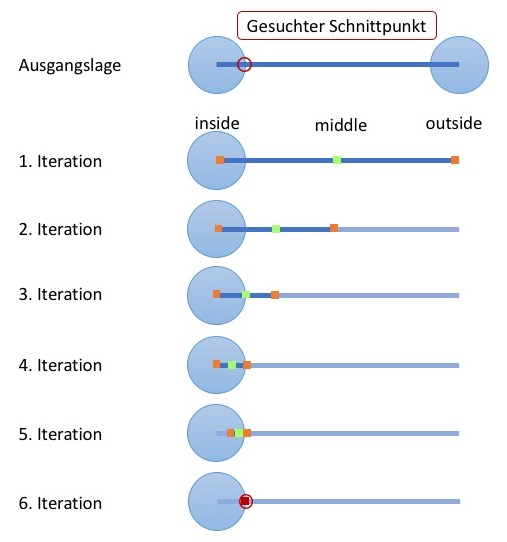
\includegraphics[width=0.6\linewidth]{assets/images/binarySearch}
		\caption{Algorithmus zur Suche eines Schnittpunktes}
		\label{fig:binarySearch}
	\end{figure}
	
	\clearpage
	\noindent
	Die spezifische Implementierung dieses Suchalgorithmus ist dem Listing \ref{code:binarySearch} zu entnehmen.
	
	\begin{lstlisting}[language=java, frame=single,caption={Algorithmus Schnittpunkt Suche}, label={code:binarySearch}]
		public Point2D findIntersectionPoint(Point2D outside, Point2D inside) {
			Point2D middle = outside.midpoint(inside);
		
			double deltaX = outside.getX() - inside.getX();
			double deltaY = outside.getY() - inside.getY();
		
			if (Math.hypot(deltaX, deltaY) < 1.) {
				return middle;
			} else {
				if (ellipse.contains(middle)) {
					return findIntersectionPoint(outside, middle);
				} else {
					return findIntersectionPoint(middle, inside);
				}
			}
		}
	\end{lstlisting}



	\section{Tree Layouter} \label{sec:treelayouter}

	Die Darstellung von Trees auf eine optisch ansprechende und leserliche Art und Weise bietet verschiedene Schwierigkeiten. Bereits 1981 haben Reingold-Tilford \cite{reingold-tilford} zu diesem Zweck einen Algorithmus entwickelt, welcher binäre Bäume zeichnet. Dieser Algorithmus wurde von Walker weiterentwickelt, um \glspl{n-ary} darzustellen und schlussendlich von Buchheim, Jünger und Leipert \cite{tree-algorithm} verbessert, um die Laufzeit auf $\mathcal{O}(n)$ zu beschränken. 
	
	Der von GVS 2.0 verwendete Algorithmus, basiert auf diesem neusten Tree-Algorithmus und genügt somit auch den fünf anerkannten Prinzipien, denen ein solcher Algorithmus genügen muss:
	
	\begin{itemize}
		\item Das Tree Layout muss die hierarchische Struktur des Trees widerspiegeln. Das heisst konkret, dass die y-Koordinate eines Knoten durch seinen Level gegeben ist.
		\item Die Knoten eines Levels sind so anzuordnen, dass sich ihre Edges nicht überkreuzen und die Knoten einen gewissen horizontalen Mindestabstand einhalten.
		\item Das Zeichnen eines Subtrees hängt nicht davon ab, an welcher Stelle im Baum sich der Subtree befindet. Das bedeutet, dass \gls{isomorph}e Subtrees identisch gezeichnet werden.
		\item Die Reihenfolge von Kindern muss im Baum ersichtlich sein. Im Falle eines binären Trees heisst das, dass ein linkes Kind links des Eltern-Knoten gezeichnet wird.
		\item Der Algorithmus arbeitet symmetrisch.
	\end{itemize}
	
	\noindent
	Ein weiterer Vorteil dieses Algorithmus ist, dass er Bäume immer so zeichnet, dass sie eine minimale Breite besitzen. Dadurch werden auch Bäume mit sehr vielen Nodes schön dargestellt. Dies führt dazu, dass der in GVS 1.0 \cite{gvs1} verwendete \textit{Cluster Splitter} nicht mehr benötigt wird. 
	
	
	
	\section{Graph Layouter}
	
	\subsection{Physics Engine} \label{ssec:graphlayouter}
	Für das Layouting der Graphen wurde ein Force-Directed Drawing Algorithm verwendet. Dieser wurde mehrheitlich von GVS 1.0 übernommen. Der Algorithmus ordnet die Vertices so an, dass es möglichst wenig überschneidende Kanten gibt. Dazu wird für jeden Vertex ein \textit{Particle} Objekt erstellt, welches während der dynamischen Plazierung auf der \textit{Area} bewegt wird. Zu Beginn des Layout Prozess wird ein Particle pseudo-zufällig platziert. Damit die Änderungen des Layouters in Echtzeit dargestellt werden, läuft der komplette Layouting Prozess in einem eigenständigen Thread. (siehe \textit{AreaTicker} in der Tabelle \ref{tbl:concurrent-classes}) Sobald ein Graph gelayouted werden muss, wird ein \textit{AreaTicker} Thread gestartet, der in einem bestimmten Intervall die Darstellung der neuen Koordinaten im UI veranlasst. Es läuft immer nur genau ein \textit{AreaTicker} Thread. Sobald sich die \textit{Particles} in der \textit{Area} stabilisiert haben, wird der \textit{AreaTicker} Thread terminiert. Das Sequenzdiagramm \ref{fig:sequencegraphlayouter} zeigt den grundlegenden Ablauf beim Starten des Graph Layout Prozess.
	
	\begin{figure}[h!]
		\centering
		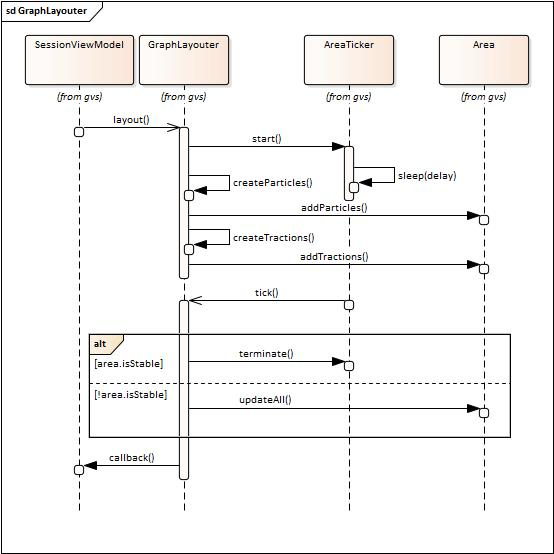
\includegraphics[width=0.6\linewidth]{assets/images/sequence_graph_layouter}
		\caption{Sequenzdiagramm: Graph Layouter}
		\label{fig:sequencegraphlayouter}
	\end{figure}
	
	\subsection{Area} \label{ssec:area}
	Die \textit{Area} dient als Container während dem dynamischen Layout Prozess. Sie beinhaltet mehrere \textit{Particle}s die von physischen Kräften bewegt werden (\textit{Traction}s und \textit{RepulsiveForce}s). Ein \textit{Particle} repräsentiert einen Vertex. Die Positionen der \textit{Particles} werden fortlaufend berechnet. Sobald ein Tick Event passiert, werden die aktuellen Koordinaten des Particles in den \textit{GraphVertex} im Business Layer kopiert. Über eine Observer Beziehung wird das \textit{VertexViewModel} im Presentation Layer über die neuen Koordinaten notifziert. Dessen X/Y Properties sind über ein bidirektionales Binding mit dem UI Element (z.B \textit{Ellipse}) verbunden. Die neuen Koordinaten werden auf der Oberfläche dargestellt. 
	
	\begin{figure}[h!]
		\centering
		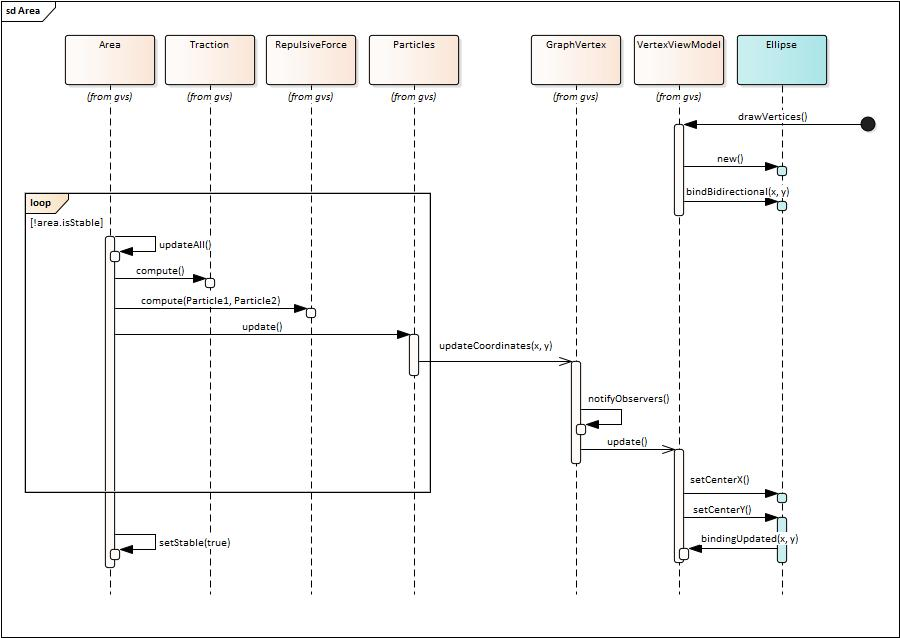
\includegraphics[width=\linewidth]{assets/images/sequence_area}
		\caption{Sequenzdiagramm: Area}
		\label{fig:sequencearea}
	\end{figure}

	\clearpage

	\section{Graph und Tree Verschmelzung} \label{graph-vs-tree}
	In theoretischer Hinsicht sind Bäume Spezialformen von Graphen. In GVS 1.0 wurden diese beiden Strukturen jedoch durchgehend getrennt modelliert. GVS 2.0 vereinigt diese Strukturen soweit es technisch Sinn macht, mit dem Ziel, Code Duplikationen weit möglichst zu vermeiden.
	
	\subsection{Unterschiede zwischen Graphen und Trees}
	\begin{itemize}
		\item Ein Graph besitzt Edges und Vertices. Ein Baum hingegen besitzt nur Vertices, denn seine Edges sind durch die Vater-Kind Beziehung der Vertices implizit gegeben. 
		\item Ein Tree Vertex besitzt zusätzliche Attribute wie Vater-Kind Beziehungen und \textit{isRoot()}
		\item Die benötigten Layout Algorithmen unterscheiden sich stark. (siehe \ref{ssec:graphlayouter} für GraphLayouter und \ref{sec:treelayouter} für TreeLayouter)
	\end{itemize}
	
	\subsection{Umsetzung}
	Auf Grund der oben genannten Unterschiede, bildet GVS 2.0 diese Strukturen wie folgt ab:
	
	\begin{itemize}
		\item Trees und Graphen werden in der Struktur \textit{Graph} vereinigt. Der \textit{ModelBuilder} erstellt für empfangene Bäume sämtliche impliziten Edges.
		\item Ein \textit{Graph} besitzt eine Liste von Vertices. Diese müssen das Interface \textit{IVertex} implementieren. Es gibt drei konkrete Implementierungen dieses Interfaces. Für reine Graphen wird die Klasse \textit{GraphVertex} benutzt. Die Klassen \textit{TreeVertex} und \textit{LeafVertex} bieten Tree-spzifische Attribute.
		\item Eine \textit{Session} umfasst jeweils mehrere \textit{Graphen}. Es gibt keine Unterscheidung zwischen Graph-Sessions und Tree-Sessions. Um einer \textit{Session} den richtigen \textit{Layouter} zuzuweisen, besitzt sie einen \textit{SessionType} der beschreibt, ob die enthaltenen Graphen effektive Graphen oder Trees sind.
		\item Nach dem Abschliessen des Layoutingprozesses ist keine Unterscheidung zwischen Trees und Graphen mehr nötig. Dies führt dazu, dass die Strukturen im Presentation Layer vollständig zusammengeführt sind.
	\end{itemize}

	
	
	\section{Watchdog} \label{sec:watchdog}
	\subsection{Bedeutung in der Informatik}
	Im  Allgemeinen versteht man in der Informatik unter einem Watchdog eine System Komponente, die andere Komponenten überwacht. Wenn in der überwachten Komponente ein Fehler auftritt, wird dieser vom Watchdog erkannt und er leitet eine angemessene Fehlerbehebung ein.\\
	Watchdogs werden vor allem in der Hardware und in der Software von Microcontrollern eingesetzt, um einen kompletten Ausfall des vom Microcontroller gesteuerten Geräts vorzubeugen.\\
	
	\subsection{Arbeitsweise}
	Während dem normalen Betrieb einer Software, wird der Watchdog regelmässig vom zu überwachendem System gefüttern. Das bedeutet, der Timer des Watchdogs wird zurückgesetzt. Beim Auftreten eines Fehlers verzögert sich diese ''Fütterung'' oder fällt gar ganz aus. Dies führt zum Ablaufen des Watchdog Timers. \\
	Sobald der Timer ausgelaufen ist, wird der Watchdog aktiv und leitet Fehlerbehebungsmassnahmen ein.
	
	\subsection{Watchdog in GVS 2.0}
	\subsubsection{Problem}
	Da per Spezifikation immer nur ein Client gleichzeitig mit dem Server kommunizieren darf, startet jeder Verbindungsaufbau mit dem Reservieren des \gls{gvsui} Services. Um den Service für andere Clients wieder frei zu geben, muss der Client nach dem Übertragen der Daten ein \textit{Release Command} senden.\\
	Der Einsatz des GVS im Unterricht findet relativ früh im Studium statt. Deshalb kommt es immer wieder einmal vor, dass sich Fehler in den Code einschleichen, welcher die \gls{gvslib} benutzt. Das Auftretten einer Programm-beendenden Exception führt dazu, dass das \textit{Release Command} nicht gesendet wird, was den GVS Service endlos blockiert. Für den Endbenutzer ist nicht ersichtlich, wieso das \gls{gvsui} nicht auf den User-Input reagiert. Einziger Ausweg bleibt, die Applikation über den Task-Manager zu beenden.
	
	\subsubsection{Lösung}
	GVS 2.0 führt einen Watchdog ein, der die Verbindung des Clients überwacht. Bei jedem Eintreffen neuer Daten, wird der Watchdog gefüttert bis er beim erhalten des \textit{Release Command}s beendet wird. Wenn nun das Auftreten einer Exception im Client Code dazu führt, dass der \textit{Release Command} nicht gesendet wird, läuft der Timer des Watchdogs aus. Dadurch wird der Watchdog aktiv und forciert das Freigeben des Services. Dieser Vorgang ist in Abbildung \ref{fig:watchdog} visualisiert.\\
	Der Endnutzer nimmt die Komplexität dieses Vorgangs nicht wahr. Nach einer Exception kann das Benutzer Programm einfach erneut gestartet werden und das \gls{gvsui} zeigt wie Erwartet die neue Session an.
	
	\begin{figure}[h!]
		\centering
		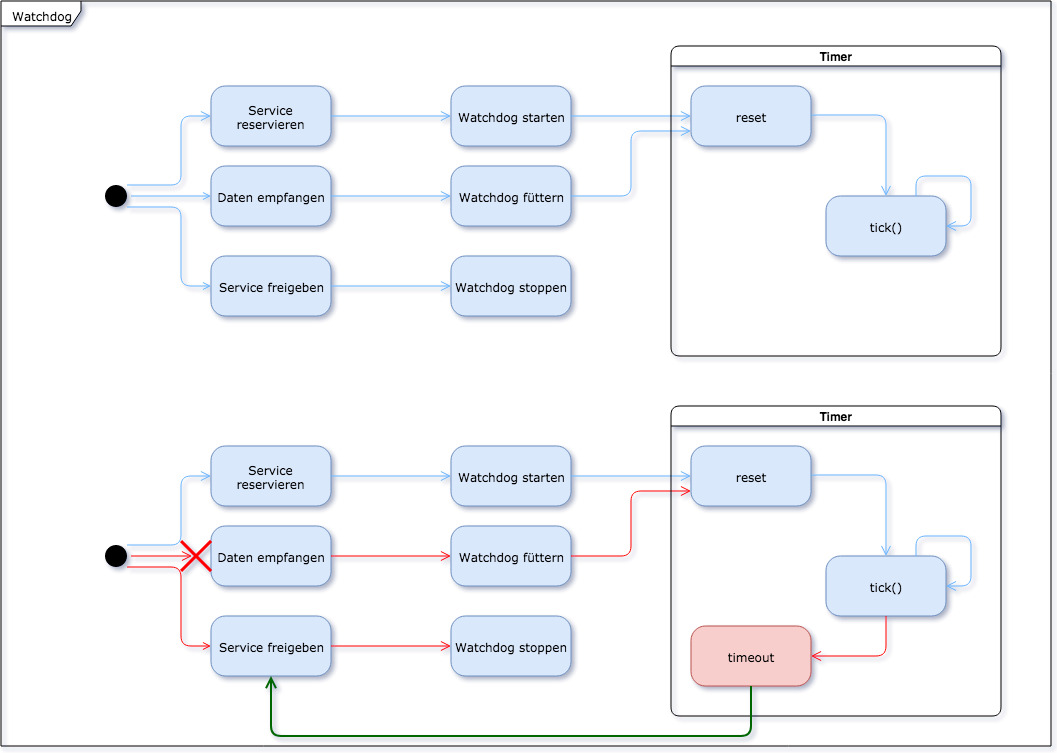
\includegraphics[width=0.7\linewidth]{assets/images/watchdog}
		\caption{GVS  2.0: Watchdog}
		\label{fig:watchdog}
	\end{figure}
	
	
	\section{Presentation Layer}
	
	\subsection{ScalablePane}
	Während der Realisierungsphase hat sich gezeigt, dass die Anzahl an Vertices in Trees und Graphen einen grossen Einfluss auf ihre Darstellung hat. Um diesen Ansprüchen gerecht zu werden, bietet GVS 2.0 eine Zeichenfläche, welche ihre Inhalte automatisch skaliert und zentriert. Dadurch werden zum Beispiel grosse Trees leserlich abgebildet und kleine Graphen verwenden die gesamte Bildschirmbreite. 
	
	\subsection{Drag Support}
	Bei Graphen können alle Vertices beliebig mit der Maus positioniert werden. Trees können nicht manuell positioniert werden. Eine entsprechende Meldung wird angezeigt.
		
	\subsection{Autolayout}
	Das Autolayout steht nur für Graphen zur Verfügung. Die Vertices werden vom Graph Layouter so positioniert, dass es möglichst wenig Überschneidungen der Edges gibt. Standardmässig ist die Einstellung \textit{Force Layout} aktiv. Dies führt dazu, dass beim betätigen des Auto-Layout Buttons die Koordinaten sämtlicher Vertices neu berechnet werden. Das Deaktivieren dieser Einstellung hat zur Folge, dass Vertices, die manuell durch den User positioniert wurden, nicht von einem Auto-Layout betroffen sind. Sollte dies auf alle Vertices zutreffen, wird der User über einen Tooltip entsprechend informiert.
		
	\subsection{UI Design}
	\begin{figure}[h!]
		\centering
		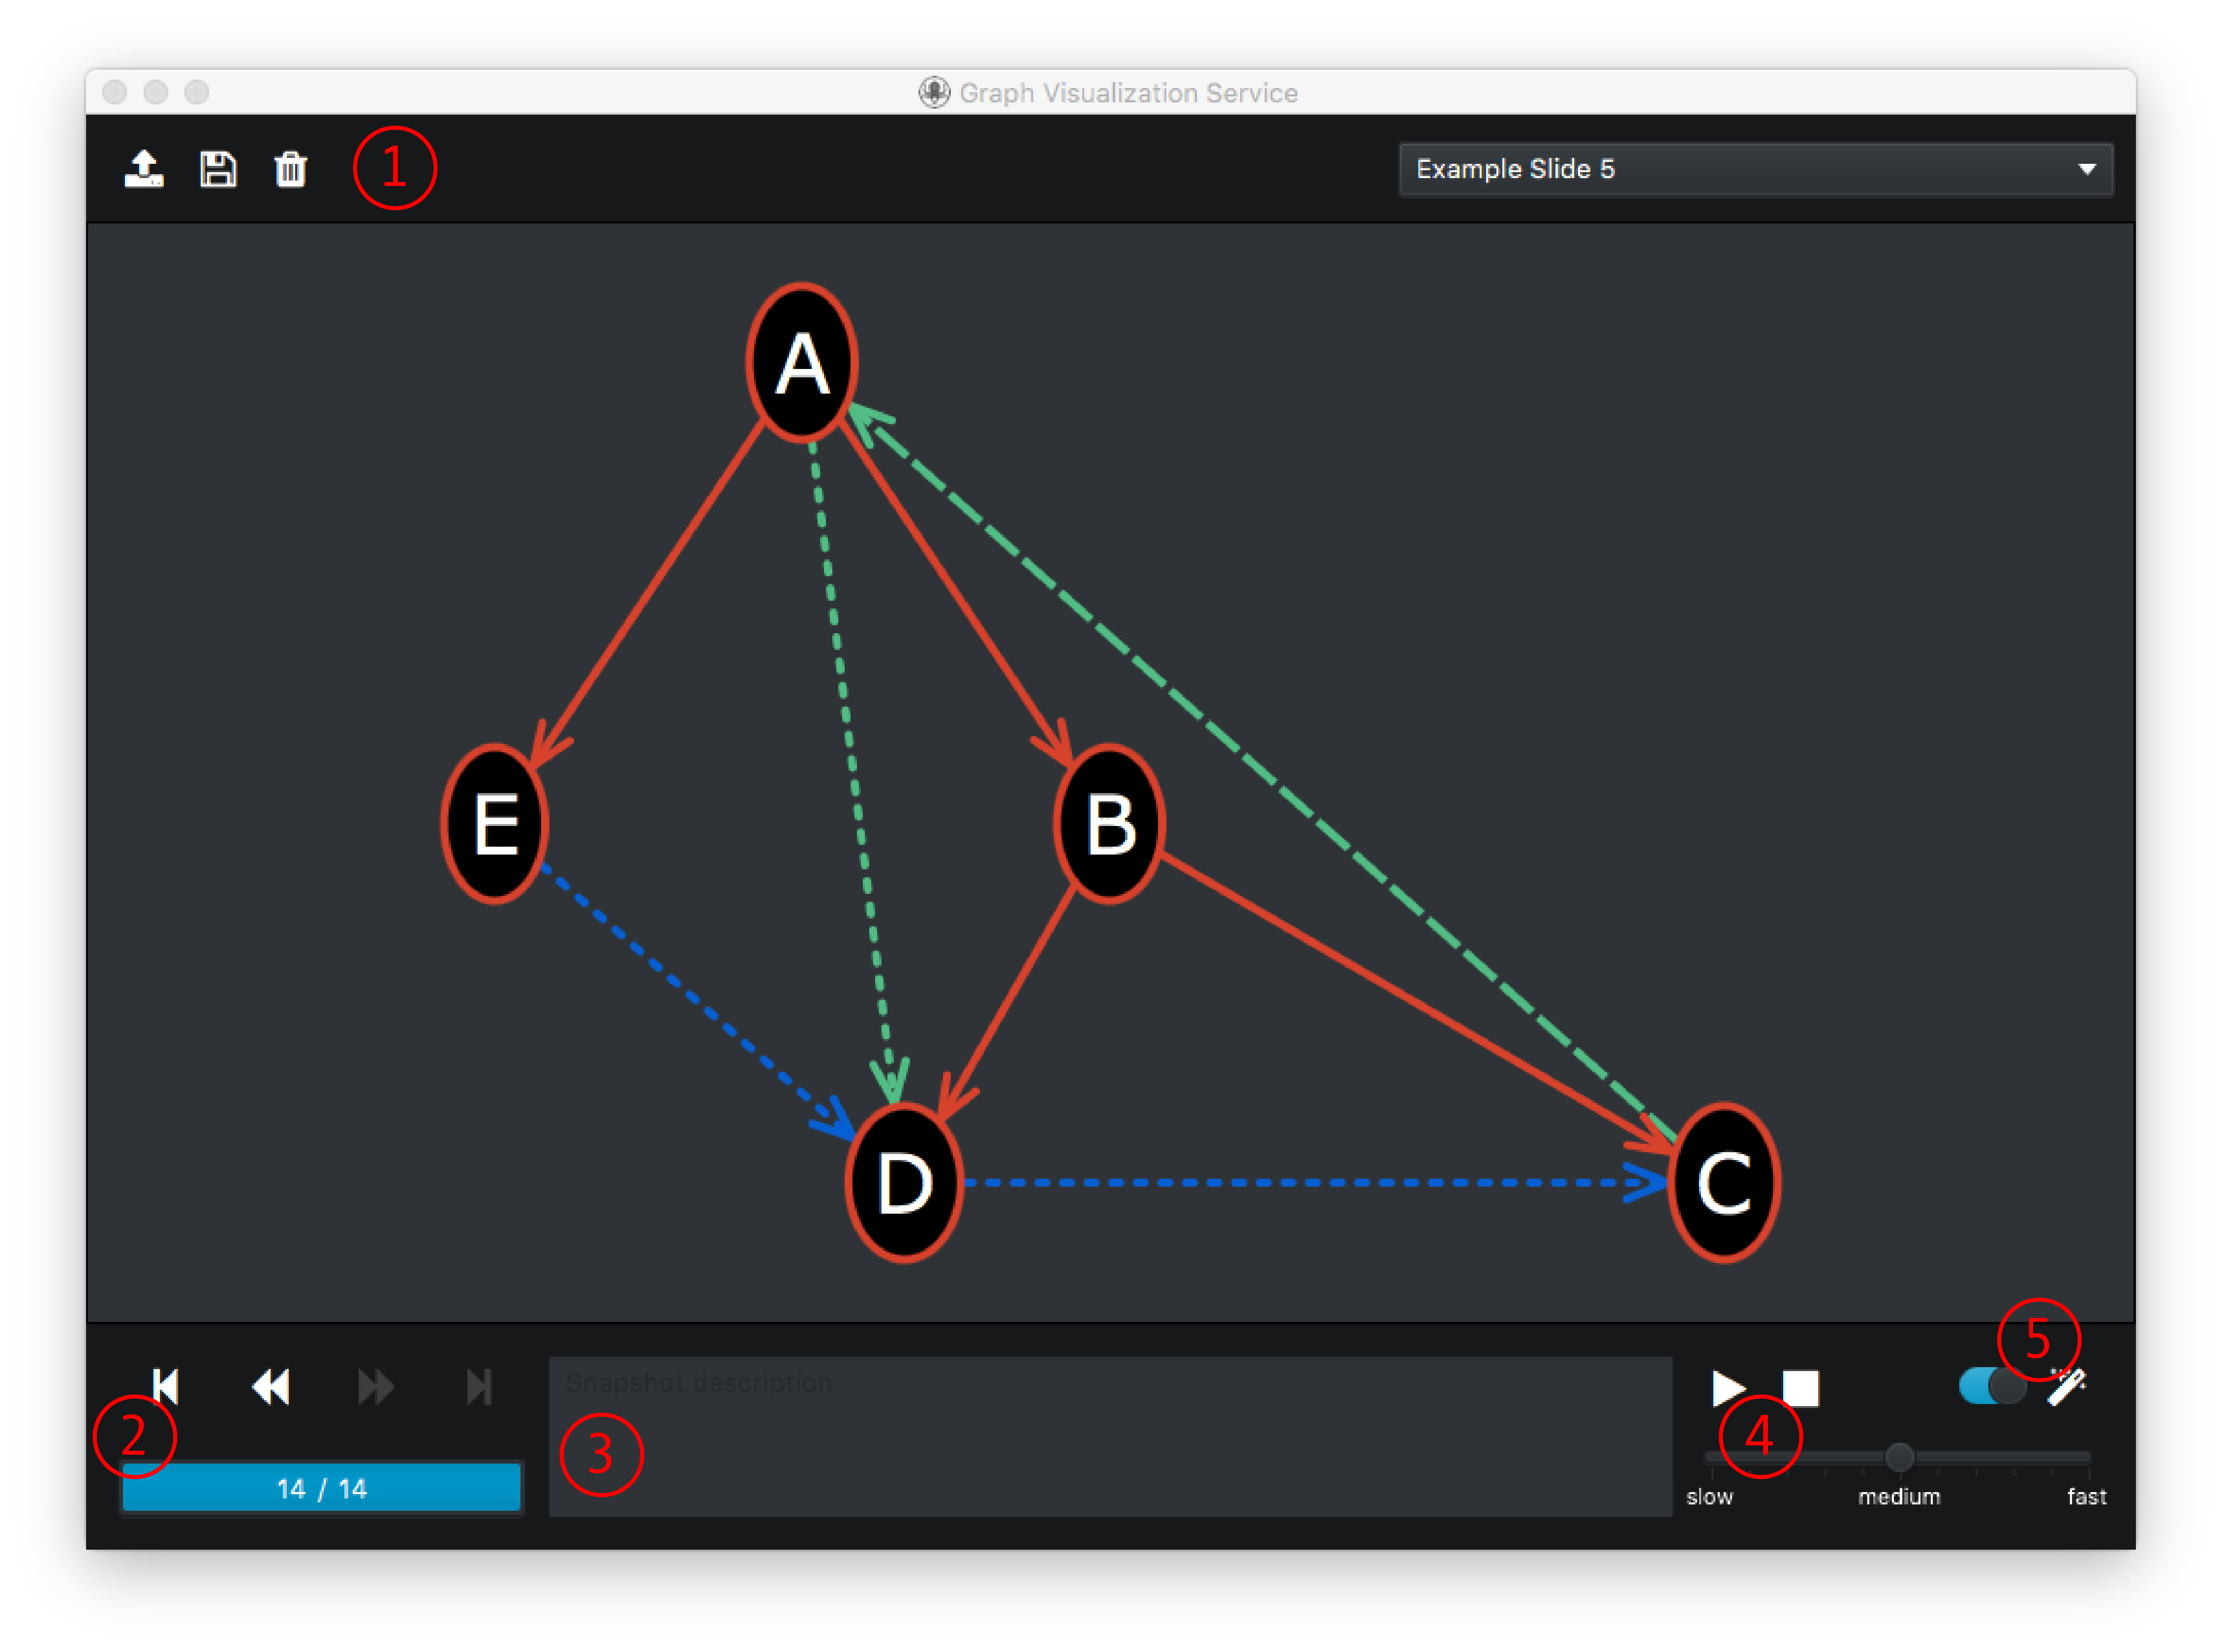
\includegraphics[width=0.7\linewidth]{assets/images/gvs-ui-graph}
		\caption{GVS 2.0: User Interface}
		\label{fig:gvs-ui-graph}
	\end{figure}

	Das User Interface orientiert sich am Aussehen des GVS 1.0. Neu sind alle wichtigen Funktionen direkt über die Toolbar zugreifbar und alle Buttons verfügen über Tooltips. Ebenfalls wurden die Zahlen des Replay Sliders durch sprechende Namen ersetzt.
	
	\subsubsection{Logo}
	Das Logo wurde von den Eigenschaften des Kraken \cite{kraken} inspiriert. Kraken sind bekannt dafür, dass sie Irrgarten-Probleme effizient lösen können. Dies ist eine Anspielung an die Algorithmen, die vom \gls{gvs} 2.0 unterstützt werden. Ebenfalls wurden die Saugnäpfe des Kraken als Graph Nodes visualisiert und auf der Stirn ist ein binärer Baum zu erkennen. 
	
	\begin{figure}[h!]
		\centering
		
\includegraphics[width=0.5\linewidth]{assets/images/logo}
		\caption[GVS Logo]{Graphs-Visualization-Service Logo}
		\label{fig:logo}
	\end{figure}
	
	\subsubsection{Farbwahl}
	Für den Hintergrund kommen bewusst dunkle Farben zum Einsatz. Dadurch werden z.B die gefundenen Pfade eines Algorithmus verstärkt farblich hervorgehoben. 
	
	
		
	\section{Client Library Upgrade}
	Für den GVS stehen Client Libraries für Java und C\# zur Verfügung. Beide Clients wurden aufgeräumt und in ein neues, versioniertes Projekt verschoben.
	
	\subsection{Generics}
	Gemäss der Aufgabenstellung (siehe Anhang \ref{aufgabenstellung}) müssen beide Clients um Generics erweitert werden. Es hat sich aber gezeigt, dass Generics auf der Schnittstelle keinen Mehrwert bieten würden (siehe Beschluss in Sitzungsprotokoll Woche 11, Anhang \ref{ch:minutes}). Schlussendlich wurden deshalb nur die intern verwendeten Listen und Maps um Generics erweitert.
	
	\subsection{Styles und Icons}
	Die von GVS 1.0 unterstützten Style-Typen wurden durch einen generellen GVS 2.0 Style ersetzt. Die Typ Klassen aus GVS 1.0 haben nur marginale Unterschiede untereinander. Mit der generellen \textit{GVSStyle} Klasse sowie vier weiteren Enums, konnte damit sehr viele duplizierter Code entfernt werden. Des Weiteren wurden die GVS 1.0 Icons durch \gls{fontawesome} Icons ersetzt. Eine Übersicht der migrierten Klassen ist der Tabelle \ref{tbl:styles} zu entnehmen.
	
	\begin{table}[h!]
		\centering
		\begin{tabularx}{\linewidth}{X X}
			\toprule 
			Klasse GVS 2.0 & Klasse GVS 1.0\\
			\midrule
			\multirow{6}{*}{GVSStyle} & 
			GVSEdgeTyp \\ & 
			GVSNodeTyp \\ & 
			GVSGraphTyp  \\ &
			GVSVertexTyp  \\ &
			GVSEllipseVertexTyp \\ &
			GVSEdgeTyp \\
			\midrule
			\multirow{2}{*}{GVSColor} & GVSEllipseVertexTyp.FillColor \\ &
			GVSDefaultTyp.LineColor \\
			\midrule
			GVSIcon & GVSIconVertexTyp \\
			\midrule
			GVSLineStyle & GVSDefaultTyp.LineStyle \\
			\midrule
			GVSLineThickness & GVSDefaultTyp.LineThickness \\
			\bottomrule 
		\end{tabularx} 
		\caption{GVS Lib: Übersicht Style Klassen} 
		\label{tbl:styles}
	\end{table}
	
	\subsection{C\# Lib Refactoring}
	In der C\# Library wurden die gleichen Änderungen wie in der Java Library durchgeführt. Zusätzlich wurde der Code um aktuelle C\# Best Practices erweitert. So werden durchgehend implizit typisierte Variablen (\lstinline|var|) verwendet, sowie der Null-Coalescing Operator (\lstinline|??|) eingesetzt. 
	
	\subsection{Layering}
	Auch in den Client Libraries wurde ein einfaches Layering eingeführt. Die Umsetzung der Schichtenarchitektur ist dem Klassendiagramm aus Anhang \ref{ch:class-diagram} zu entnehmen.	


	\section{Weitere Änderungen gegenüber GVS 1.0}
	Dieser Abschnitt umfasst kleinere Änderungen, Neuerungen und Fehlerbehebungen gegenüber dem Vorgänger Produkt \cite{gvs1}.
	
	\subsection{Änderungen}
	\begin{description}
		\item[MaxLabelLength] \hfill \\
		In GVS 1.0 wurde eine MaxLabelLength vom Client an den Server übermittelt. In GVS 2.0 ist dieser Wert in der \textit{Configuration} Klasse als Konstante definiert. Da er vor allem Einfluss auf das Layout der Trees hat, ist dieser Wert in GVS 2.0 nicht mehr konfigurierbar. Erhält der GVS 2.0 mit zu langen Labels, werden diese automatisch durch Auslassungspunkte in der Mitte des Labels gekürzt.
		\item[Background] \hfill \\ 
		Für Graphen bestand in GSV 1.0 die Möglichkeit, ein Background Bild festzulegen. Da diese Funktionalität im Unterricht nicht verwendet wird, wurde sie nach Rücksprache mit dem Betreuer ersatzlos entfernt.
		\item[Icon \& IconVertex] \hfill \\
		Anstelle der Icon Bilder, die für Knoten in GVS 1.0 ausgewählt werden konnten, bietet GVS 2.0 neu sämtliche Icons von \gls{fontawesome} \cite{fontawesome} an. Zudem gibt es serverseitig keine Unterscheidung zwischen Vertices mit und ohne Icon, was die Klasse \textit{IconVertex} überflüssig macht.
		\item[CORBA] \hfill \\
		Gemäss Vereinbarung mit dem Betreuer (siehe Anhang \ref{ch:minutes}) wurde die Verbindungsoption über CORBA entfernt.
		\item[Log Level Konfiguration] \hfill \\
		Die Log Level können in GVS 2.0 nicht mehr über das User Interface konfiguriert werden. Stattdessen kann das Log Level mittels \gls{jmx} und der JConsole oder durch Anpassen der Logback Konfiguration verändert werden. Dieses Vorgehen ist im Benutzerhandbuch (siehe Anhang \ref{ch:manual}) genauer beschrieben.
	\end{description}

	\subsection{Neuerungen} \label{ssec:neuerungen}
	\begin{description}
		\item[SnapshotDescription] \hfill \\ 
		Damit einzelne Schritte in den dargestellten Graphen besser verständlich sind, bietet GVS 2.0 die Möglichkeit kurze Beschreibungen zu erfassen. Diese können serverseitig erfasst, gespeichert und geladen werden. Die Erweiterung des Verbindungsprotokoll, um SnapshotDescription auch clientseitig zu unterstützen, sollte für ein allfälliges Folgeprojekt geplant werden (siehe Kapitel \ref{sec:ausblick}).
		\item[n-ary Trees] \hfill \\
		Der Tree Layout Algorithmus von GVS 2.0 ist fähig neben Binary Trees auch \glspl{n-ary} zu zeichnen (siehe \ref{sec:treelayouter}). Da der nötige Code clientseitig bereits vorhanden war, konnte das \gls{gvsui} mit kleinen Aufwand erweitert werden. Somit können in GVS 2.0 nun auch allgemeinere Trees, wie z.B. \glspl{trie}, dargestellt werden.
	\end{description}
	
	\subsection{Fehlerbehebungen}
	\begin{description}
		\item[Watchog] \hfill \\ 
		In GVS 1.0 haben Exceptions im Client Code (der die GVS Lib benutzt) nicht zu einem Verbindungsabbruch geführt. Der Server blieb reserviert und ein neu gestarteter Client konnte keine Verbindung aufbauen. Für den User war nicht ersichtlich, wieso der Server auf den neuen Input nicht reagiert. Um dieses Usability Problem zu beheben bietet GVS 2.0 einen Watchdog Thread. Dieser überwacht die Verbindung und erzwingt einen Verbindungsabbruch, wenn sich der Client längere Zeit nicht mehr meldet. Mehr zum Watchdog unter \ref{sec:watchdog}.
		\item[Speicherort]  \hfill \\ Der Speicherort für Sessions war in GVS 1.0 hart kodiert. Dies führte auf UNIX Systemen zu einem Fehlverhalten. In GVS 2.0 kann der User den Speicherort für seine Sessions selber wählen.
		\item[Entfernung der Root] \hfill \\ Die GVS Lib bietet zwei Unterschiedliche Strukturen um Trees darzustellen. Bei Benutzung der Struktur \textit{GVSTreeWithRoot} kam es zu Fehlern, wenn die Root auf \textit{null} gesetzt wurde. In GVS 2.0 ist dieser Fehler behoben.
	\end{description}

	

	\chapter{Ergebnisdiskussion} \label{ch:ergebnisse}
	\begin{table}[h!]
		\centering
		\begin{tabularx}{\linewidth}{l l X l}
			\toprule 
			Datum & Version & Änderungen & Autor \\
			\midrule
			11.12.17 & 1.0 & Ausblick geschrieben & mtrentini \\
			11.12.17 & 1.1 & Metriken geschrieben & mwieland \\
			15.12.17 & 1.2 & Zielerreichung geschrieben & mtrentini \\
			\bottomrule 
		\end{tabularx} 
		\caption{Versionshistory Ergebnisdiskussion} 
	\end{table}	
	
	
	
	\section{Zielerreichung}
	Dieses Kapitel reflektiert die Erreichung der gemäss Aufgabenstellung (siehe Anhang \ref{aufgabenstellung}) gesetzten Ziele dieser Arbeit. Neben den subjektiven Einschätzungen des Projektteams dienen die benutzten Metriken als handfeste Grundlage für qualitative Verbesserungen.
	
	\subsection{Ersetzung des Presentation Layers}
	GVS 1.0 benutzt UI-spezifische \gls{swing} und \gls{awt} Klassen in sehr vielen Komponenten und durch alle Layer hinweg (siehe \ref{sssec:swing-business}). Insbesondere deshalb war das Ersetzen des Presentation Layers keine kleine Aufgabe. Schnell hat sich gezeigt, dass weniger Code als erwartet wiederverwendet werden kann. Im Zuge dieser Ersetzungen von Swing und AWT Klassen durch GVS spezifische Klassen, wurden auch viele kleinere Refactorings umgesetzt. Diese Umstände haben auch dazu geführt, dass es zu Abweichungen gegenüber der geplanten Migration der Klassen gekommen ist (siehe Anhang \ref{ch:migration-list})\\
	Die neue Architektur von GVS 2.0 konnte sämtliche \glspl{tangle} entwirren (siehe \ref{ssec:layering}) und glänzt mit einem in sich gekoppelten Presentation Layer.
	
	Für den Endbenutzer wirkt das neue User Interface frisch und modern. Durch die direkte Erreichbarkeit aller Funktionen über die Toolbar, ist es auch benutzerfreundlicher als das UI des Vorgängers.
	
	\subsection{Einführung von Generics in \gls{gvslib}}
	Im Laufe des Projekts wurde erkannt, dass die \gls{gvslib} bereits einige Generics-Neuerungen enthält und eine weitere Einführung derselben keinen namhaften Mehrwert bringen würde. Somit wurde in Rücksprache mit dem Betreuer entschieden, dass diesbezüglich keine Änderungen an der \gls{gvslib} nötig sind (siehe Anhang \ref{ch:minutes}).\\
	Stattdessen konnten die zahlreichen Style-Typ Klassen von GVS 1.0 auf eine einzige Style Klasse (analog zu \gls{gvsui}) reduziert werden, was wiederum zukünftige Erweiterungen der Applikation erleichtert.
	
	\subsection{Punktuelle Verbesserungen}
	Wie im Kapitel \ref{ch:umsetzung} beschrieben, konnten zahlreiche Verbesserungen durchgeführt werden. Von besonderem Nutzen sind hierbei zwei Verbesserungen. Einerseits die Umsetzung einer klaren Schichtenarchitektur, die zukünftigen Entwicklern das Ersetzen einzelner Komponenten erleichtern wird. Andererseits das Einführen eines Watchdogs, welcher die Usability für Studenten stark erhöht, da Exceptions im Implementations-Code nicht mehr zur Blockierung des \gls{gvsui} führen.
	
	\subsection{Bedürfnisse der Stakeholder}
	Wie in Kapitel \ref{ssec:stakeholder} beschrieben, gibt es für den \gls{gvs} drei relevante Stakeholder. Das in dieser Arbeit entstandene Endprodukt deckt die Bedürfnisse dieser Stakeholder ab.
	
	\begin{itemize}
		\item Für Studenten entstand eine modern anmutende und intuitiv bedienbare Applikation mit verbesserter Fehlertoleranz (siehe Kapitel \ref{sec:watchdog} \textit{Watchdog}).
		\item Zukünftige Entwickler wird die Erweiterung oder Ersetzung einzelner Teile der Applikation durch die umgesetzte Schichtenarchitektur erleitert.
		\item Der Dozent kann die Applikation wie gewohnt einsetzen. Sämtliche bisherigen Übungen die auf \gls{gvs} setzen, finden sich in einer erneuerten Version im \textit{Testers} Repository \cite{gvs-tester}.
	\end{itemize}
	
	\section{Software Metriken} \label{sec:metrics-2}
	In der Analyse Phase wurden mehrere Code Smells in GVS 1.0 erkannt (Siehe Abschnitt \ref{sec:erkenntnisse}). In der Design Phase wurde deshalb ein Konzept ausgearbeitet, damit das Refactoring strukturiert ablaufen wird (Siehe Abschnitt \ref{sec:refactoring-concept}). Die Refactorings wurden damals aus Zeitgründen tief priorisiert. Es hat sich aber gezeigt, dass bereits am Anfang der Realisations Phase viele Refactorings durchgeführt werden müssen. Dies nicht zuletzt deshalb, da der bestehende Code sehr schwer zu lesen war. Durch die Refactorings konnte die Verständlichkeit des Codes enorm verbessert werden. Dies spiegelt sich auch in den erhobenen Software Metriken wieder. Im folgenden Abschnitt sind diese genauer beschrieben.
	
	\subsection{Wartbarkeit}
	In der Wartbarkeits-Metrik \cite{metric-maintainability} ist klar zu erkennen, dass die Wartbarkeit der meisten Klassen gut ist. Auf der X-Achse ist der Churn \cite{metric-churn} abgebildet, also wie oft eine Klasse verändert wurde. Klassen die oft angepasst werden, erledigen potentiell zu viele Aufgaben. Auf der Y-Achse ist die Wartbarkeit angezeigt. Diese errechnet sich aus Code-Duplikationen, zyklomatischer Komplexität von McCabe \cite{mccabe} und der Kognitiven Komplexität \cite{metric-cognitive-complexity} einer Klasse. Die beiden Klassen \textit{Persistor} und \textit{ModelBuilder} weisen die schlechtesten Werte auf (oben rechts). Leider konnte aus Zeitgründen kein Refactoring der beiden Klassen durchgeführt werden. Ein entsprechender Hinweis ist aber im Ausblick \ref{ssec:gvs-todos} dokumentiert.
	
	\clearpage
	
	\begin{figure}[h!]
		\centering
		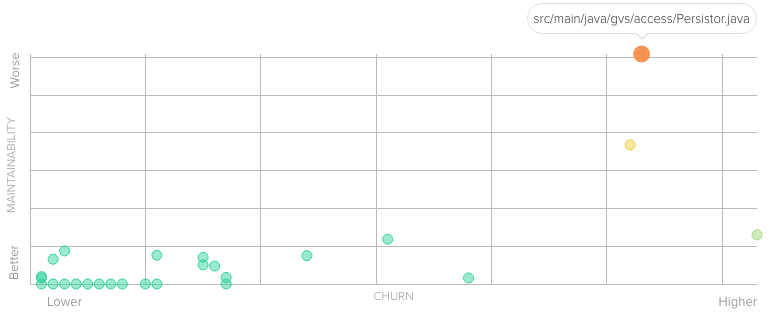
\includegraphics[width=\linewidth]{assets/images/metrics/maintainability}
		\caption{Metrik: Wartbarkeit}
		\label{fig:metric-maintainability}
	\end{figure}
	
	\subsection{Technische Schulden}
	Technischen Schulden (Abb. \ref{fig:metric-technical-debt}) beschreiben den zusätzlichen Aufwand, welcher für die Korrektur von schlecht geschriebenen Software aufgewendet werden muss. Die Metrik korreliert mit den Anzahl Zeilen an Source Code (Siehe \ref{ssec:lines-code}). Auch gut zu erkennen ist, dass die technischen Schulden trotz weiteren Anpassungen nicht mehr zugenommen haben.
	\begin{figure}[h!]
		\centering
		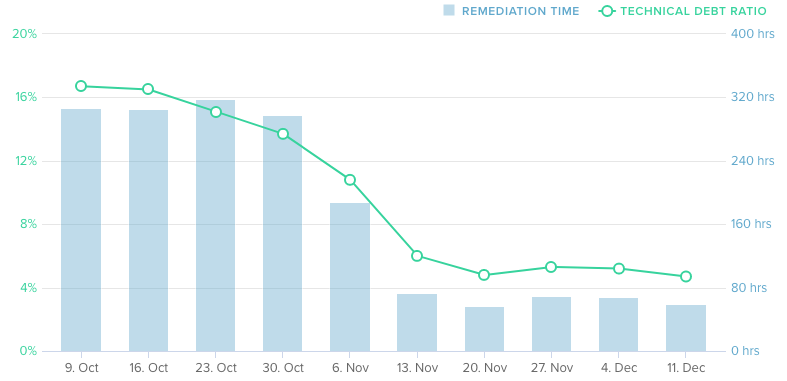
\includegraphics[width=\linewidth]{assets/images/metrics/technical_debt}
		\caption{Metrik: Technische Schulden}
		\label{fig:metric-technical-debt}
	\end{figure}
	
	\subsection{Lines of Code} \label{ssec:lines-code}
	Interessant zu beobachten ist, dass beinahe die selbe Funktionalität mit viel weniger Zeilen Code erreicht wurde. Dies ist insbesondere durch das Entfernen von dupliziertem Code möglich. Ein weiterer Einfluss hat der Einsatz von modernen Lambda Ausdrücken, die zur Zeit der Entwicklung von GVS 1.0 nicht zur Verfügung standen.
	\begin{figure}[h!]
		\centering
		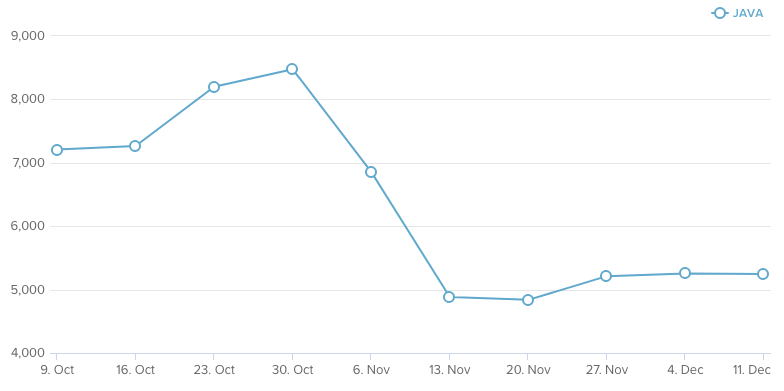
\includegraphics[width=\linewidth]{assets/images/metrics/lines_of_code}
		\caption{Metrik: Lines of Code}
		\label{metric-linesofcode}
	\end{figure}	

	
	\subsection{Kritik}
	In der Analyse- und Entwurfsphase des Projekts wurde entschieden, dass die Hauptziele so umgesetzt werden sollen, dass möglichst viel bestehender Code wiederverwendet werden kann. Dieses Ziel wurde klar nicht erreicht.\\
	Dies führte auch dazu, dass deutlich mehr Arbeitsaufwand für die Umsetzung des Projekts nötig war, als eingeplant wurde (siehe Anhang \ref{zeitauswertung}). Die Wirtschaftlichkeit des Projekts hat dadurch gelitten.\\
	
	\noindent
	Des Weiteren hat sich das Projektteam zu Beginn stark mit der Verbesserung der Architektur und Code Qualität beschäftigt. Dadurch gingen gewisse Feinheiten der Funktionalität etwas unter. Als Beispiel kann hier genannt werden, dass erst relativ spät klar wurde, wozu einige Einstellungen aus dem Kontextmenü - wie der Cluster Splitter oder das Soft-Layout - dienen.



	\section{Ausblick}
	\label{sec:ausblick}
	Obwohl viel erreicht wurde im GVS 2.0 Projekt, konnten nicht alle Ideen umgesetzt und sämtliches Verbesserungspotential ausgeschöpft werden.
	
	\noindent
	Dieses Kapitel bietet eine Übersicht, welche Aufgaben in einem nächsten GVS Major Update angegangen werden könnten. 
	
	\subsection{Verbesserungspotential GVS 1.0}
	Während der Verwendung von GVS 1.0 sind einige Dinge aufgefallen, die nicht optimal funktionieren. Diese wurden vom Betreuer in einer Liste festgehalten und an das Projektteam überreicht. Gemäss der Besprechung vom 27.09.2017 wurden diese Änderungen mit tiefer Priorität in den Backlog eingepflegt (siehe Anhang \ref{ch:minutes}). Dieses Kapitel zeigt auf, welche Punkte bis zum Abschluss des Projekts offen geblieben sind.
	
	\begin{description}
		\item[Font Size] \hfill \\
			GVS 3.0 sollte es dem User erlauben die Font Size der Labels zu verändern, ohne den Code von \gls{gvsui} zu bearbeiten. Eignen würde sich entweder ein Menü-Eintrag ''Einstellungen'' oder das setzen von der Font Size in der \textit{GVSStyle} Klasse.
		\item[Unicode Labels] \hfill \\
		GVS 3.0 sollte die Darstellung von Unicode Zeichen in Labels unterstützen.
		\item[Snapshot Description] \hfill \\
			GVS 2.0 bietet einem User die Möglichkeit, eine Notiz zu einem Snapshot zu verfassen (siehe \ref{ssec:neuerungen}).\\
			GVS 3.0 sollte das verwendete Protokoll und die \gls{gvslib} Klassen so erweitern, dass solche Notizen direkt im Client erstellt und mit den Graphen mitgeschickt werden können.
		\item[Schnelle Beendigung der GVS Lib] \hfill \\
			Wenn die \textit{main} Methode des Programms, welches GVS Lib verwendet sehr schnell beendet, gehen Daten bei der Übertragung verloren. Dies sollte bei GVS 3.0 verhindert werden.
	\end{description}
	
	\subsection{Nicht umgesetzte Ideen im GVS 2.0}
	\label{ssec:gvs-todos}
	\begin{description}
		\item[Refactoring ModelBuilder und Persistor] \hfill \\
			Die Klassen \textit{ModelBuilder} und \textit{Persistor} besitzen sehr ähnliche Funktionalität und somit viel \textit{duplicated Code}. Obwohl diese Klassen in GVS 2.0 einem Refactoring unterzogen wurden, besteht das Problem weiterhin (siehe Abschnitt \ref{sec:metrics-2}).\\
			GVS 3.0 sollte diese Klassen soweit refactoren, dass kein \textit{duplicated Code} mehr vorhanden ist.
		\item[Automated Testing] \hfill \\
			GVS 1.0 besitzt keine automatisierten Tests. Auch in GVS 2.0 konnte diese Altlast nicht beseitigt werden. Es wurde nur eine sehr kleine Test Coverage erreicht, da die Erstellung von automatisierten Tests tief priorisiert wurde.\\
			GVS 3.0 sollte den Business Layer und Teile des Access Layers sinnvoll mit Tests abdecken.
	\end{description}
	
	
	\newpage
	
	\appendix
	\noappendicestocpagenum
	\addappheadtotoc
	\appendixpage
	
	\chapter{Projektplanung}
	
	\begin{table}[h!]
		\centering
		\begin{tabularx}{\linewidth}{l l X l}
			\toprule 
			Datum & Version & Änderungen & Autor \\
			\midrule
			25.09.17 & 1.0 & Dokument erstellt & mwieland, mtrentini \\
			28.09.17 & 1.1 & Risikomanagement hinzugefügt & mtrentini \\
			03.10.17 & 1.2 & IDE, Frameworks, Buildprozess, Qualitätsmanagement hinzugefügt, & mwieland \\
			05.10.17 & 1.3 & Meilensteine definiert & mtrentini \\
			11.12.17 & 1.4 & Verantwortlichkeiten festgehalten & mtrentini \\
			\bottomrule 
		\end{tabularx} 
		\caption{Versionshistory Projektplanung} 
	\end{table}
	
	
	
	\section{Meilensteine}
	\label{sec:milestones}
	
	\subsubsection{Meilenstein 1: Analyse}
	Analyse des Ist-Zustandes von GVS 1.0: Die Problemdomäne wird spezifiziert. Mehrere Diagramme zeigen die Schnittstelle zwischen dem Business Layer und dem Presentation Layer auf. Es ist ersichtlich, wie die einzelnen Komponenten miteinander kommunizieren bzw. wie die Daten von der Socket ans UI weiter gereicht werden.\\
	Die in der Aufgabenstellung (\ref{aufgabenstellung}) geforderten Requirements werden festgehalten.
	
	\subsubsection{Meilenstein 2: Entwurf}
	\label{milestone2}
	Entwurf des Soll-Zustand von GVS 2.0: Eine klassische 3-Schichten Architektur wird entworfen. Es wird spezifiziert, welche GVS 1.0 Komponenten durch welche GVS 2.0 Komponenten ersetzt werden. 
	
	\subsubsection{Meilenstein 3: Release 1}
	Der Presentation Layer ist vollständig gemäss Punkt 1 im Refactroing Konzept (\ref{sec:refactoring-concept}) umgesetzt.
	
	\subsubsection{Meilenstein 4: Release 2}
	Die im Refactoring Konzept (\ref{sec:refactoring-concept}) beschlossenen Änderungen sind umgesetzt. Das mit dem Enterprise Architekt erstellte Klassendiagramm ist mit dem Stand der GVS 2.0 Software synchron.
	
	\subsubsection{Meilenstein 5: Release 3}
	Alle im Meilenstein 2 definierten Requirements sind umgesetzt. Die GVS 2.0 Software ist für den Einsatz im Unterricht bereit.
	
	\begin{table}[h!]
		\centering
		\begin{tabular}{l l l l}
			\toprule 
			\# & Name & Artefakte & Datum \\
			\toprule 
			1 & Analyse & Anforderungsspezifikation & 11.10.17 \\
			& & Klassendiagramm 1.0 & \\
			& & Sequenzdiagramme & \\
			& &  Systemübersichts-Diagramm & \\
			\midrule
			2 & Entwurf  & Designspezifikation & 25.10.17\\
			& & Klassendiagramm 2.0 & \\
			& & Migrationstabelle & \\
			\midrule
			3 & Release 1 & GVS 2.0.1 & 22.11.2017 \\
			\midrule
			4 & Release 2 & GVS 2.0.2 & 06.12.2017 \\
			\midrule
			5 & Release 3 & GVS 2.0.3 & 22.12.2017 \\
			\bottomrule 
		\end{tabular} 
		\caption{Meilenstein Planung} 
	\end{table}
	
	\subsection{Artefact Overview}
	Im Artefact Overview sind sämtliche zu erbringende Arbeitsergebnisse mit ihren Fertigstellungsdaten aufgelistet. Wenn nötig sind verschiedene Versionen gekennzeichnet.
	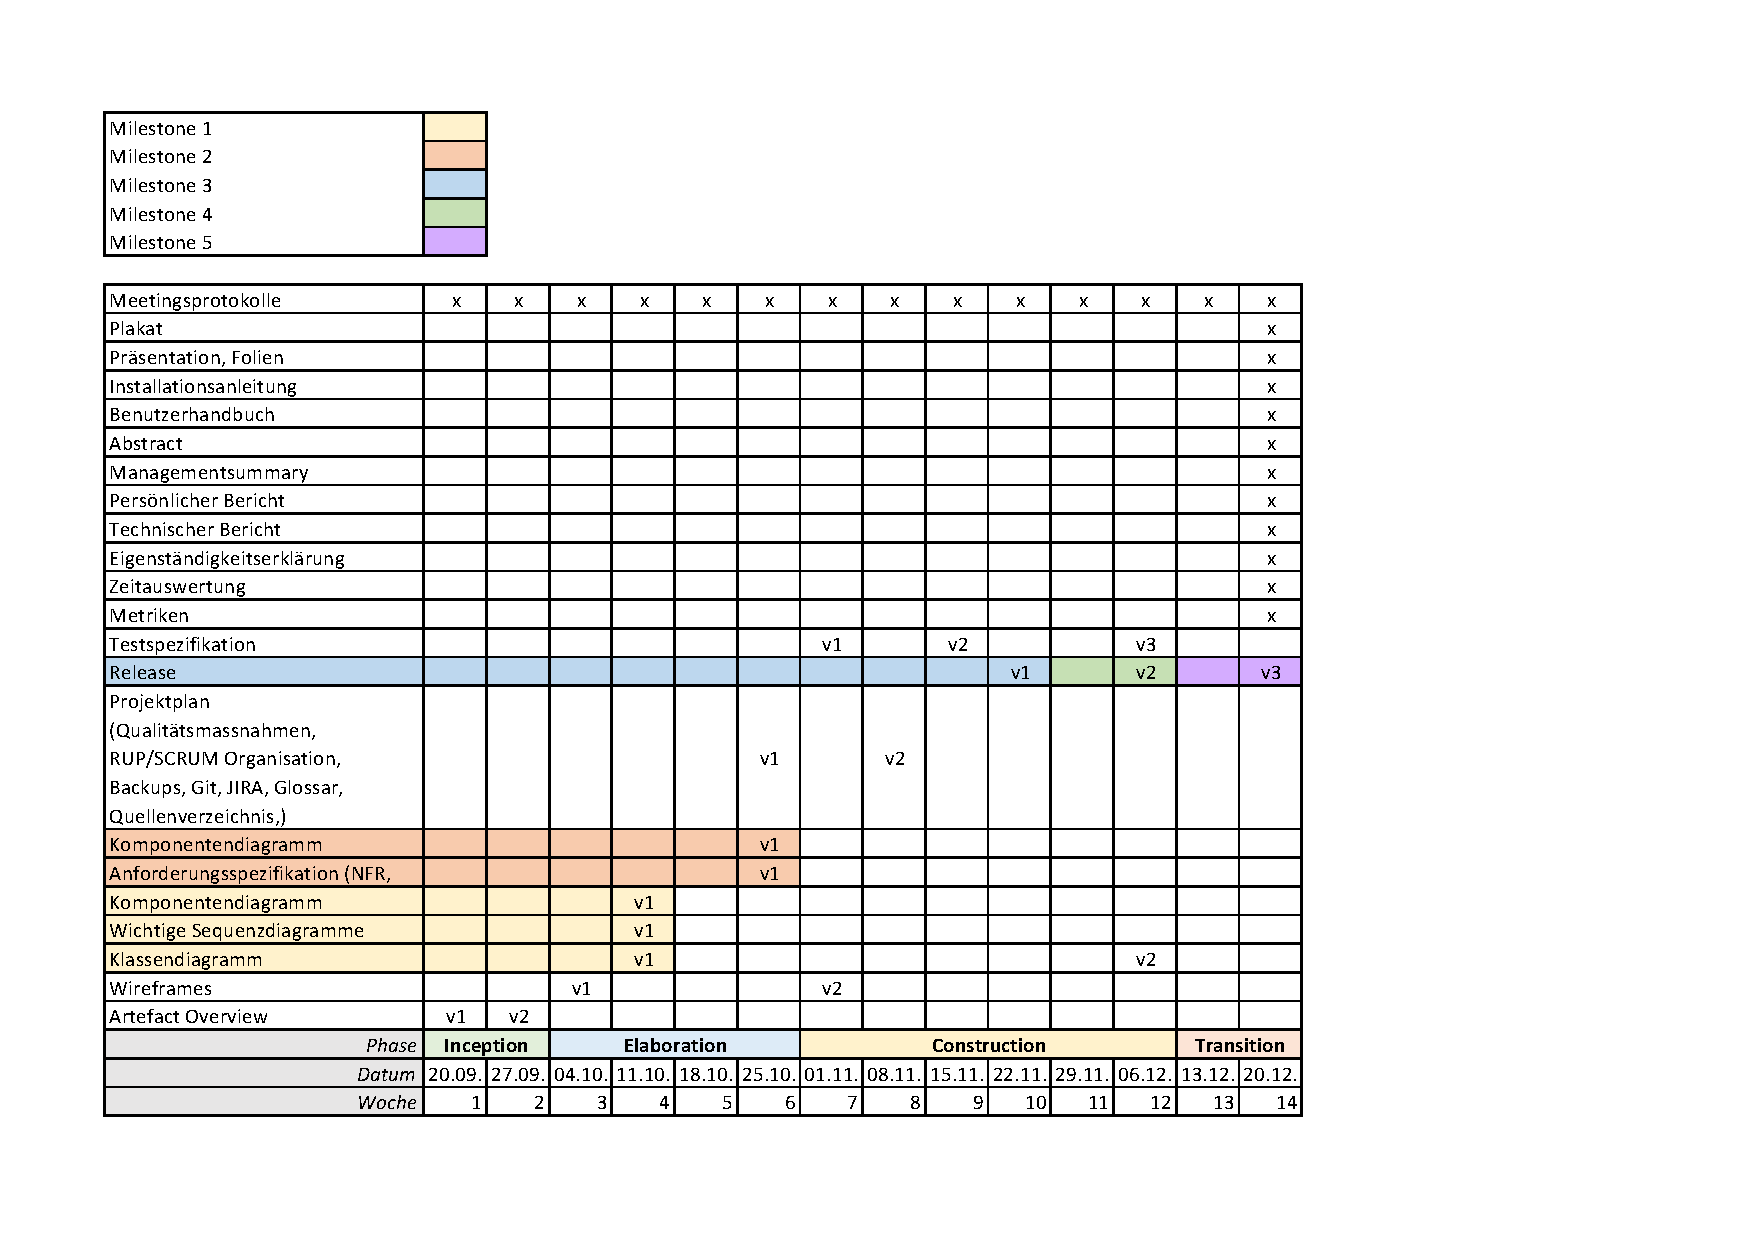
\includepdf[landscape]{assets/pdf/artefact_overview.pdf}
	
	
	
	\section{Zeitplanung}
	
	Das Projekt wird im Rahmen der Studienarbeit durchgeführt. Insgesamt stehen 14 Wochen zur Verfügung in welchen jedes Teammitglied 240 Stunden leisten muss. Somit entstehen ca. 17 Stunden Arbeitsaufwand pro Woche und Teammitglied.
	
	
	
	\section{Projektverwaltung}
	
	Als Projektmanagement Software wird Jira \cite{jira} eingesetzt. In Jira werden alle Requirements als Issues erfasst und in den Product Backlog eingepflegt. Pro Iteration sollen jeweils so viele Issues eingeplant werden, wie unter Berücksichtigung von administrativen Aufgaben abgearbeitet werden können. Dabei spielt der Teamspeed eine grosse Rolle, welcher sich über die Projektdauer einpendeln soll. 
	
	
	\subsection{Iterationsplanung}
	Die Iterationsplanung orientiert sich grob am \gls{rup} und ist unterteilt in eine Inception-, Elaboration-, Construction- sowie eine Transition-Phase. Jede Phase besteht aus einer oder mehreren Iterationen, die jeweils 1 Wochen dauern und am Donnerstag enden. Die Sprints sind bewusst nur 1 Woche lang, um eventuell ändernden Anforderungen gerecht zu werden. Zudem bringen die Wochenmeetings (\ref{ssec:meeting}) jeweils neuen Input, welcher dann direkt in den nächsten Sprint einfliessen kann.\\
	Eine Iteration wird nach \gls{scrum} organisiert. Am Anfang des Sprints definiert das Projektteam die zu erledigenden Issues und schätzt deren Aufwand. (Siehe \ref{sec:estimations}) Jeweils am Ende eines Sprints wird die geleistete Arbeit reflektiert. Entsprechende Erkenntnisse und Verbesserungen werden fortlaufend in die Projektorganisation aufgenommen. 
	
	\subsection{Schätzungen}
	\label{sec:estimations}
	Issues werden auf Basis von Story Points geschätzt. Dieses Vorgehen hat sich mit SCRUM etabliert. Die Nutzung von Story Points führt dazu, dass nicht die individuell unterschiedliche Bearbeitungszeit, sondern die Komplexität einer User Story geschätzt wird. Dies vereinfacht  und homogenisiert die Schätzungen und hilft den Teamspeed zu bestimmen.\cite{storypoints, storypoints2}
	
	\subsection{Zeitauswertung}
	Für die Zeitauswertung wird das Jira Plugin Tempo \cite{jiratempo} verwendet. Dieses bietet umfassende Auswertungsmöglichkeiten, sowie Exports nach MS Excel. Die Reports zur geleisteten Zeit befinden sich im Anhang \ref{zeitauswertung}.
	
	\subsection{Meetings} \label{ssec:meeting}
	Über die gesamte Projektdauer findet jeweils am Mittwoch um 17:15 ein wöchentliches Standortmeeting statt. Die Beschlüsse aus den Meetings werden protokolliert und bis spätestens 24h später an alle Teilnehmer versendet. Allfälliges Feedback wird nachträglich eingepflegt und versioniert abgelegt.
	
	\subsection{Branch Konzept}
	Die Branch Struktur orientiert sich an Gitflow \cite{gitflow}. Pro Issue wird ein Feature Branch erstellt, der nach erfolgreichem Review in den Development Branch gemerged wird. Beim Erreichen eines Meilensteins (siehe \ref{sec:milestones}) wird der Entwicklungszweig in den Master Branch gemerged.
	
	
	
	\section{Entwicklungsumgebung}
	Als \gls{ide} wird Eclipse mit folgenden Plugins verwendet
	\begin{itemize}
		\item Buildship \cite{buildship} für die Gradle Integration
		\item EGit \cite{egit} für die Git Integration
		\item ECLEmma \cite{eclemma} zur Überprüfung der Testabdeckung
		\item FindBugs \cite{findbugs} zur statischen Code Analyse
		\item Stan4J \cite{stan4j} zur Überprüfung von zyklischen Abhängigkeiten
		\item Checkstyle \cite{checkstyle} zur Überprüfung der Coding Richtlinien.
	\end{itemize}
	
	
	
	\section{Frameworks}
	
	\subsection{Gluon Ignite mit Google Guice} \label{DI}
	Gluon Ignite \cite{gluonignite} erweitert das verbreitete \gls{di}-Framework Guice \cite{guice} für den Einsatz in \gls{javafx} Applikationen. Mit Gluon Ignite lässt sich \gls{di} nicht nur im Business Layer, sondern auch für die \gls{fxml} Loader verwenden. \gls{di} verringert die Kopplung zwischen Komponenten, verbessert die Testbarkeit und zentralisiert die Erzeugungslogik von Klassenobjekten.
	
	\subsection{ControlsFX}
	ControlsFX \cite{controlsfx} ist ein Open Source Projekt für JavaFX UI Controls. Es erweitert die Standard-Controls um nützliche Elemente. Im GVS 2.0 wird es für den Toggle Button verwendet. 
	
	\subsection{dom4j}
	Dom4j \cite{dom4j} ist ein XML Framework für Java. Es wird für das Schreiben und Lesen der XML Files verwendet, die über die Socket Verbindung gesendet werden.
	
	\subsection{SLF4J und Logback}
	SLF4J \cite{slf4j} und Logback \cite{logback} werden das Schreiben von Log Einträgen in ein File sowie auf die Standardausgabe (STDOUT) verwendet.
	
		
		
	\section{Repositories}
	Die Artefakte werden in verschiedenen Repositories auf GitHub versioniert abgelegt. So gibt es für die Dokumentation, die Meetings-Protokolle und den Sourcecode jeweils ein eigenes Repository.
	
	\begin{table}[h!]
		\centering
		\begin{tabularx}{\linewidth}{l l X}
			\toprule 
			Repository & Nutzen & URL \\
			\midrule
			gvs-ui & UI und Socket Server & \url{https://github.com/Graphs-Visualization-Service/gvs-ui}  \\
			gvs-lib-java & Library für Java Programme & \url{https://github.com/Graphs-Visualization-Service/gvs-lib-java} \\
			gvs-lib-csharp & Library für C\# Programme & \url{https://github.com/Graphs-Visualization-Service/gvs-lib-csharp} \\
			gvs-tester & Ausführbare End-to-End Testfiles in Java & \url{https://github.com/Graphs-Visualization-Service/gvs-tester} \\
			\bottomrule 
		\end{tabularx} 
		\caption{GVS 2.0 Repositories} 
		\label{tbl:repos}
	\end{table}
	
	\section{Continuous Integration}
	Die Software wird nach jedem Commit mit Travis CI \cite{travisci} gebuildet. Dies garantiert, dass sämtliche Qualitätsmassnahmen stets eingehalten werden. (Siehe \ref{sec:qualitymeasures})
	
	\subsection{Buildprozess}
	\label{sec:buildprocess}
	Zur Erstellung der Software Artefakte wird Gradle \cite{gradle} eingesetzt. Gradle verwaltet alle externen Software Abhängigkeiten. Zusätzlich wird die Software nur dann gebuildet, wenn alle Metriktools grünes Licht geben. Es resultiert ein ausführbares \gls{jar}.
	
	
	
	\section{Qualitätsmanagement}
	\label{sec:qualitymeasures}
	
	\subsection{Unit und System Tests}
	Zur Sicherung der Software Qualität sind gute Tests unerlässlich. Da jedoch ein grosser Teil des Business Layers von GVS 1.0 übernommen wird, ist es nicht realistisch, für sämtliche Klassen Unit Tests nachzureichen. Wo immer möglich und sinnvoll sollen automatisierte Tests geschrieben werden. Der Schwerpunkt liegt dabei auf der Qualität und nicht auf einer möglichst hohen Testabdeckung.
	
	Des Weiteren ist ein grosser Teil der Applikation an die Benutzeroberfläche gekoppelt. Diese Teile können nur schwer mit automatisieren Tests abgedeckt werden. Deshalb soll mit End-zu-End Tests der gesamte Funktionsumfang getestet und protokolliert werden (siehe Anhang \ref{Testprotokoll}).
	
	\subsection{Definition of Done} \label{ssec:dod}
	Source Code wird erst zum Review freigegeben, wenn folgende Kriterien erfüllt sind.
	\begin{itemize}
		\item Die \gls{ide} rsp. Build Tool zeigt keine Warnungen und Fehler
		\item Es gibt keinen auskommentierten Code
		\item Es existieren sinnvolle Unit und Integrationstests für das Feature
		\item Alle Metriken geben grünes Licht
		\item Das Issue wurde in Jira \cite{jira} zum Review vermerkt
	\end{itemize}
	
	\subsection{Review}
	Nach Abschluss eines Issues wird dieses an den Teampartner zum Review übergeben. Durch das Vier-Augen-Prinzip kann die Qualität des Produktes hoch gehalten werden. Zusätzlich haben beide Teampartner stets den selben Wissensstand.
	
	\subsection{Metriken} \label{ssec:metriken}
	Mit den Metriken kann während der Entwicklung geprüft werden, ob die Code Qualität den gesetzten Vorgaben (Siehe \ref{ssec:dod}) entspricht.
	
	\begin{description}
		\item[Code Style] \hfill \\
		Als Styleguide wird eine angepasste Version des Sun Styleguide verwendet \cite{suncheckstyle}. Damit dieser im Projekt durchgängig eingehalten wird, wird das Checkstyle Plugin \cite{checkstyle} in den Build-Prozess integriert. (Siehe \ref{sec:buildprocess})
		\item[Code Climate] \hfill \\
		Zur Überwachung des Technical Debt und der Wartbarkeit wird die Github App Code Climate \cite{codeclimate} eingesetzt.	
	\end{description}
	
	\subsection{Refactorings}
	Aufgrund der erkannten Mängel in der Analysephase (Siehe \ref{sec:erkenntnisse}) werden fortlaufend Refactorings des migrierten Codes durchgeführt.
	
	
	
	
	\section{Risikomanagement}
	Nachfolgend sind die wichtigsten Risiken für diese Arbeit aufgelistet. Gewichtet werden die Risiken nach Eintrittswahrscheinlichkeit und Schadenshöhe. \cite{risikomanagement} Auf eine Schätzung bezüglich dem zeitlichen Mehraufwand wird bewusst verzichtet, da diese erfahrungsgemäss sehr ungenau ist und wenig praktischen Nutzen hat. Dennoch erzwingt die Liste ein aktives Auseinandersetzen mit den möglichen Risiken und zeigt Wege für die Eskalation rsp. Reaktion beim Eintritt eines Risikos.
	
	\begin{table}[h!]
		\centering
		\begin{tabular}{l c c}
			\toprule 
			\# & Eintrittswahrscheinlichkeit (E) & Schadensschwere (S) \\
			\toprule 
			1 & gering & leicht  \\
			2 & mittel & mittelschwer \\
			3 & hoch & schwer \\
			\bottomrule 
		\end{tabular} 
		\caption{Legende Risiken} 
	\end{table}
	\begin{landscape}		
		\subsection{Mögliche Risiken}
		\begin{table}[h!]
			\centering
			\begin{tabularx}{\linewidth}{l X l l X X}
				\toprule 
				\# & Beschreibung & E & S & Prävention & Massnahmen bei Eintritt \\
				\toprule 
				1 & Verlust von Daten auf Grund von technischen Störungen oder Diebstahl von persönlichen Notebooks & 2 & 1 & Backups (siehe \ref{sec:backup}) & Durch die Massnahmen muss höchstens ein Datenverlust von 8h aufgearbeitet werden. \\
				\midrule
				2 & Die Schnittstelle zwischen Business Logik und Presentation Layer ist weitaus weniger wohldefiniert als ursprünglich angenommen. Der nötige Zeitaufwand übersteigt die Schätzung um ein Vielfaches & 1 & 2 & Gute Recherche und Einarbeit in GVS 1.0, genügend lange Elaboration Phase & Rücksprache mit Betreuer. Überprüfen des Projektscopes und allenfalls Anpassung des Scopes. \\
				\midrule
				3 & Funktionalitäten von GVS 1.0, welche mit Swing umgesetzt wurden, werden durch \gls{javafx} nicht oder unzureichend unterstützt & 1 & 2 & Einlesen in JavaFX \cite{javafxbook}, Funktionalitäten GVS 1.0 abklären & Alternative zur bestehenden Umsetzung finden \\
				\midrule
				4 & Eingesetzte Frameworks, Libraries und Cloud Services harmonieren nicht wie angenommen & 2 & 2 & Auf einen Software Stack setzen, der beliebt und weit verbreitet ist. Dies reduziert das Risiko, dass der gegenseitige Support fehlt. & Alternativen für inkompatible Services finden \\  
				\midrule 
				5 & Der geplante Funktionsumfang von GVS 2.0 übersteigt das Zeitbudget, dass im Rahmen der Studienarbeit zur Verfügung steht & 2 & 3 & Endprodukt in Teilkomponenten aufteilen. Pro Komponente den zeitlichen Aufwand bewerten. Klare Definition, welche Artefakte zwingend umgesetzt werden müssen. & Frühzeitige Rücksprache mit dem Betreuer, wenn sich abzeichnet, dass eine Komponente mehr Arbeit in Anspruch nimmt. \\  
				\bottomrule 
			\end{tabularx} 
			\caption{mögliche Risiken} 
		\end{table}
	\end{landscape}
	
	\subsection{Backups}
	\label{sec:backup}
	Zur Minimierung von allfälligen Datenverlusten wird wie folgt vorgegangen:
	
	\begin{enumerate}
		\item Täglich automatisiertes Backup aller Projektdaten im JIRA \cite{jira} (Zeiterfassung, erstellte Issues, JIRA Konfiguration)
		\item Die Projektdokumentation sowie der Programmcode wird in den vier Github Repositories der Github Organisation \cite{github} versioniert abgelegt. (Siehe Tabelle \ref{tbl:repos}) Für die Projektmitglieder gilt der Grundsatz ''Commit early and often''.
		\item Weitere Artefakte werden auf Dropbox \cite{dropbox} abgelegt und dort automatisch gesichert und versioniert.
	\end{enumerate}
	
	
	
	\section{Verantwortlichkeiten}
	Um Unklarheiten und Unstimmigkeiten zu vermeiden sind folgende Verantwortlichkeiten zugeteilt:
	
	\begin{table}[h!]
		\centering
		\begin{tabular}{l l}
			\toprule 
			Bereich & Verantwortliche/r \\
			\toprule 
			Analyse & beide \\
			Design & beide \\ 
			Testing (Usability, Systemtests) & mtrentini \\
			Projektmanagement (inkl. Protokolle) & beide \\
			Entwicklungsumgebung, CI & mwieland \\
			\bottomrule 
		\end{tabular} 
		\caption{Verantwortlichkeiten} 
	\end{table}
	
	\noindent
	Alle Team-Mitglieder arbeiten jedoch in allen Bereichen des Projekts mit. 
	Die genaue Arbeitsteilung ist der git-History, den Java-Docs sowie den Änderungshistories in der Projektdokumentation zu entnehmen.
	
	\chapter{Klassendiagramme} \label{ch:class-diagram}
	Die folgenden Seiten enthalten die Entwicklung der Klassendiagramme über den Projektverlauf. Für die \gls{gvslib} Komponente existierte in der Vorgängerarbeit kein Klassendiagramm.
	
	\begin{enumerate}
		\item GVS 1.0 Klassendiagramm UI Analyse
		\item GVS 2.0 Klassendiagramm UI Entwurf
		\item GVS 2.0 Klassendiagramm UI Umsetzung
		\item GVS 2.0 Klassendiagramm Lib Umsetzung
	\end{enumerate}
	
	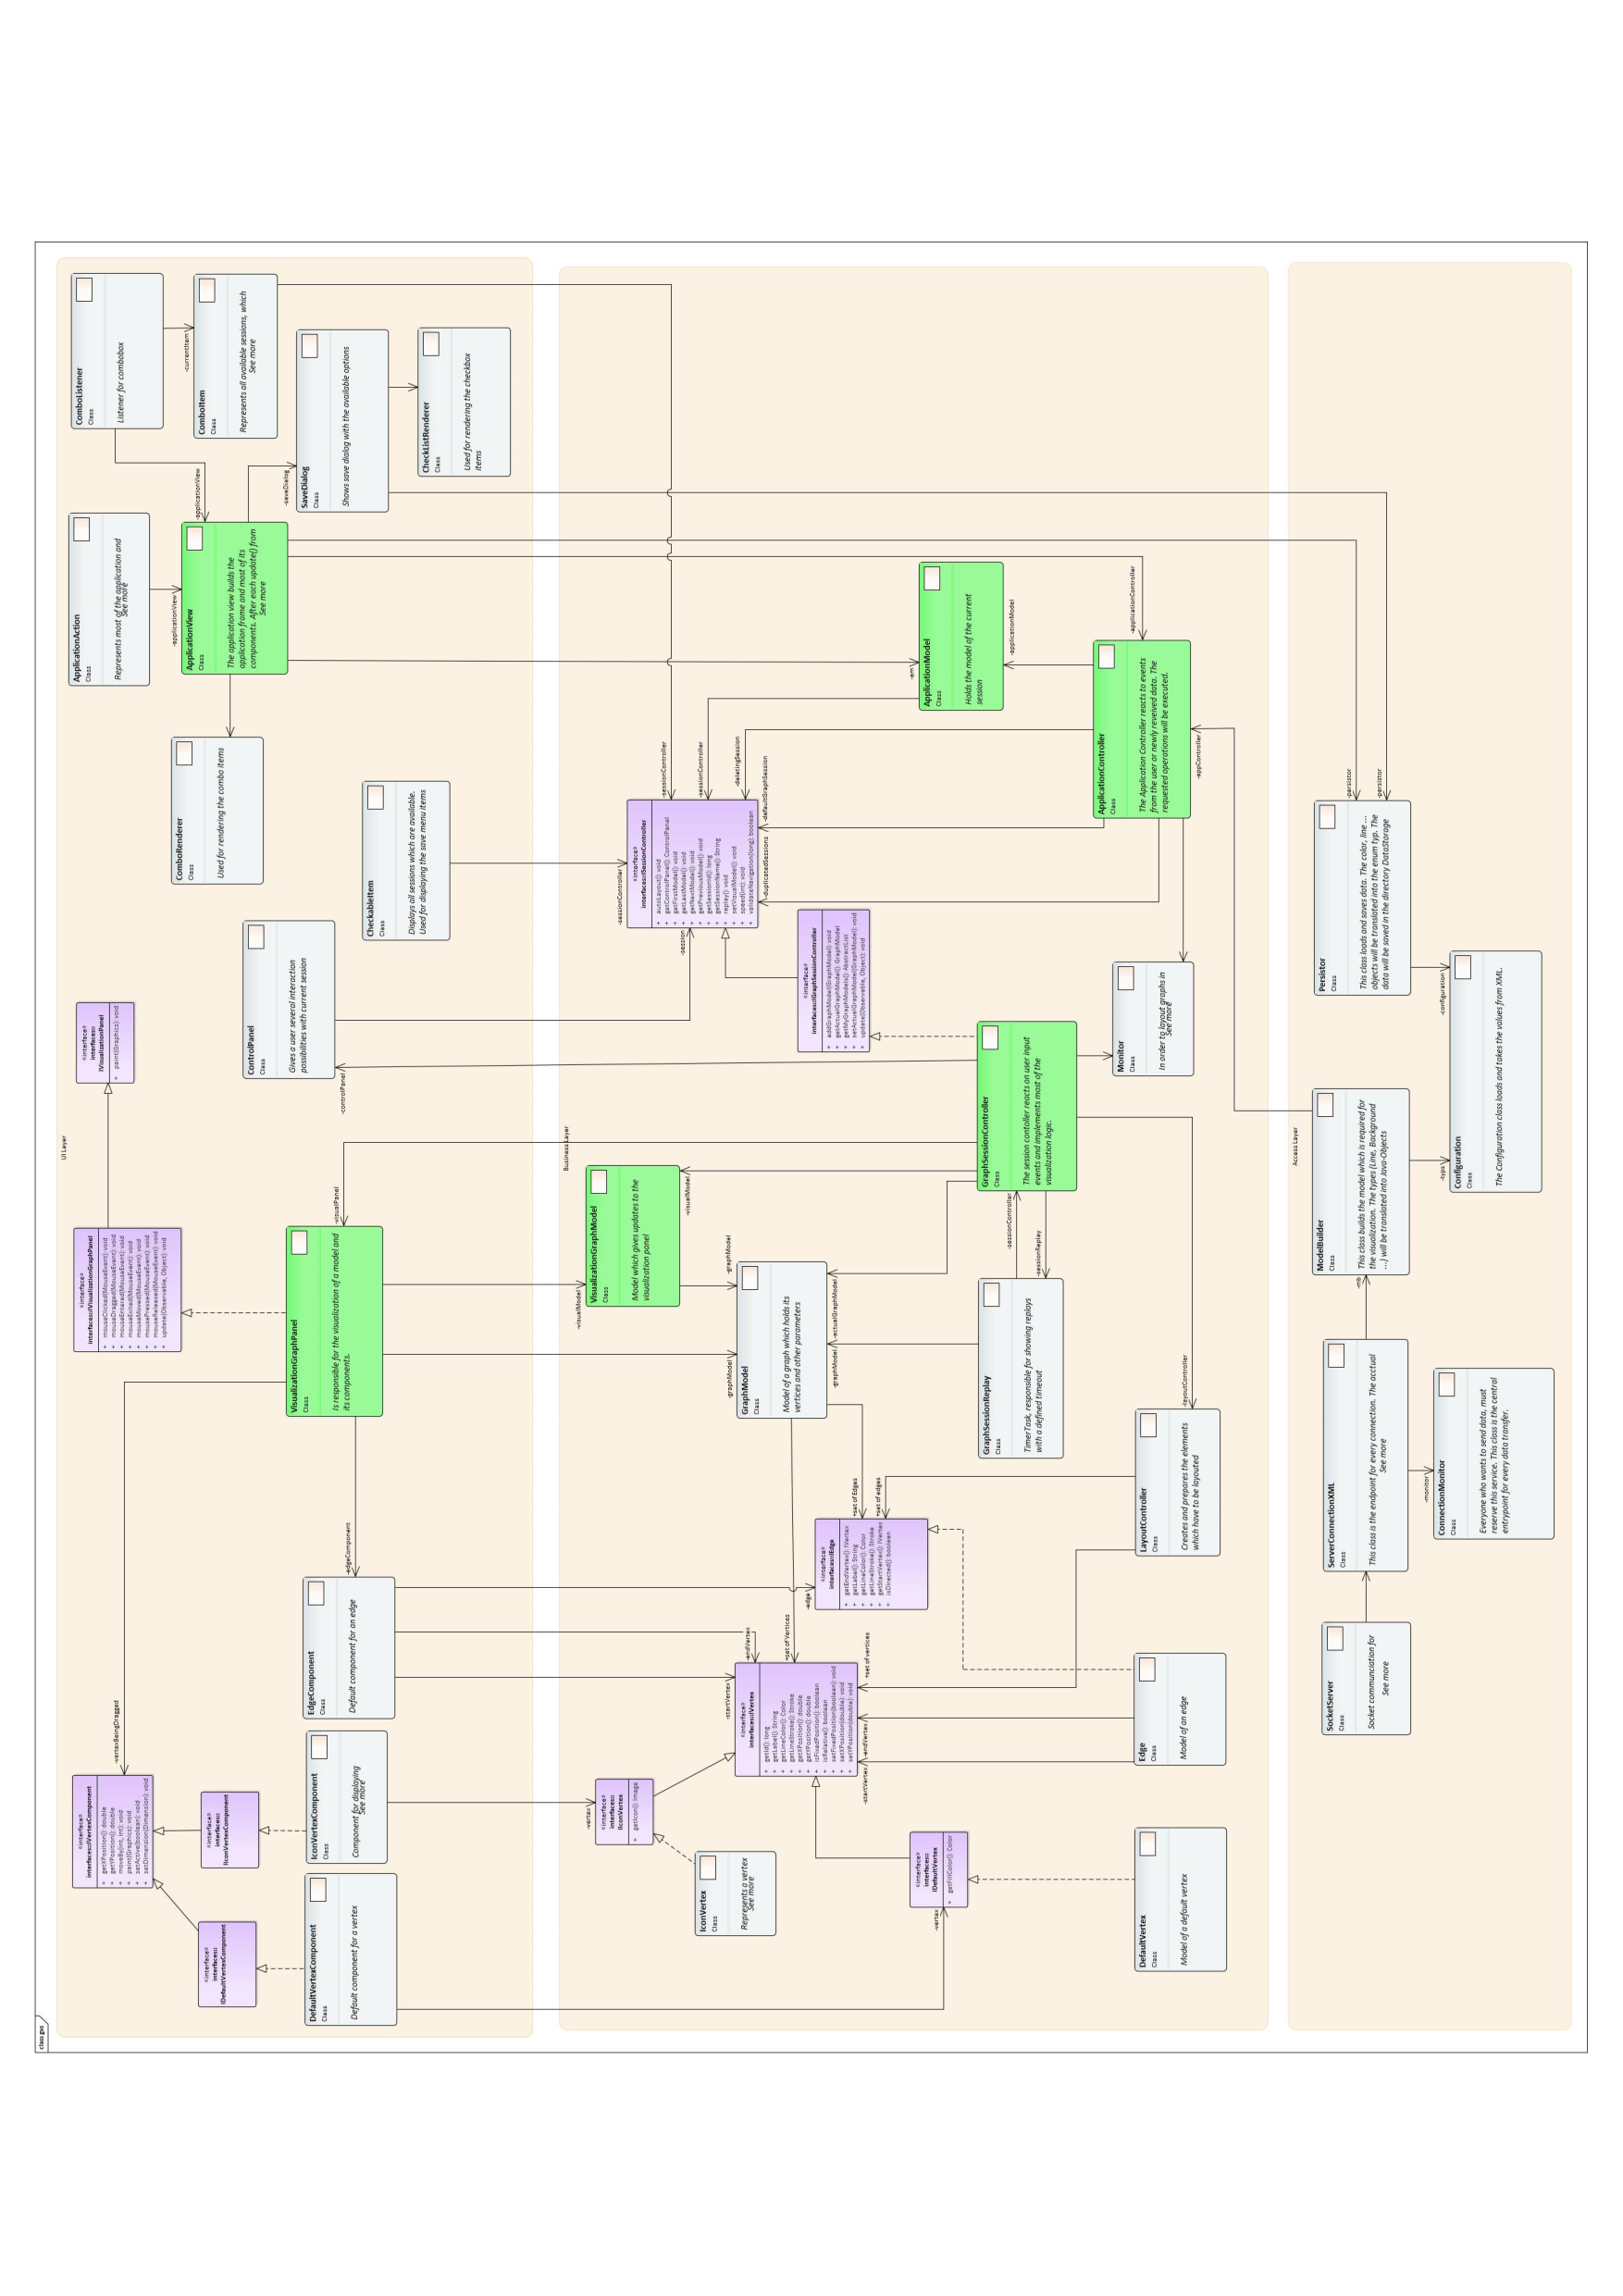
\includepdf[fitpaper]{assets/pdf/gvs1-0.pdf}
	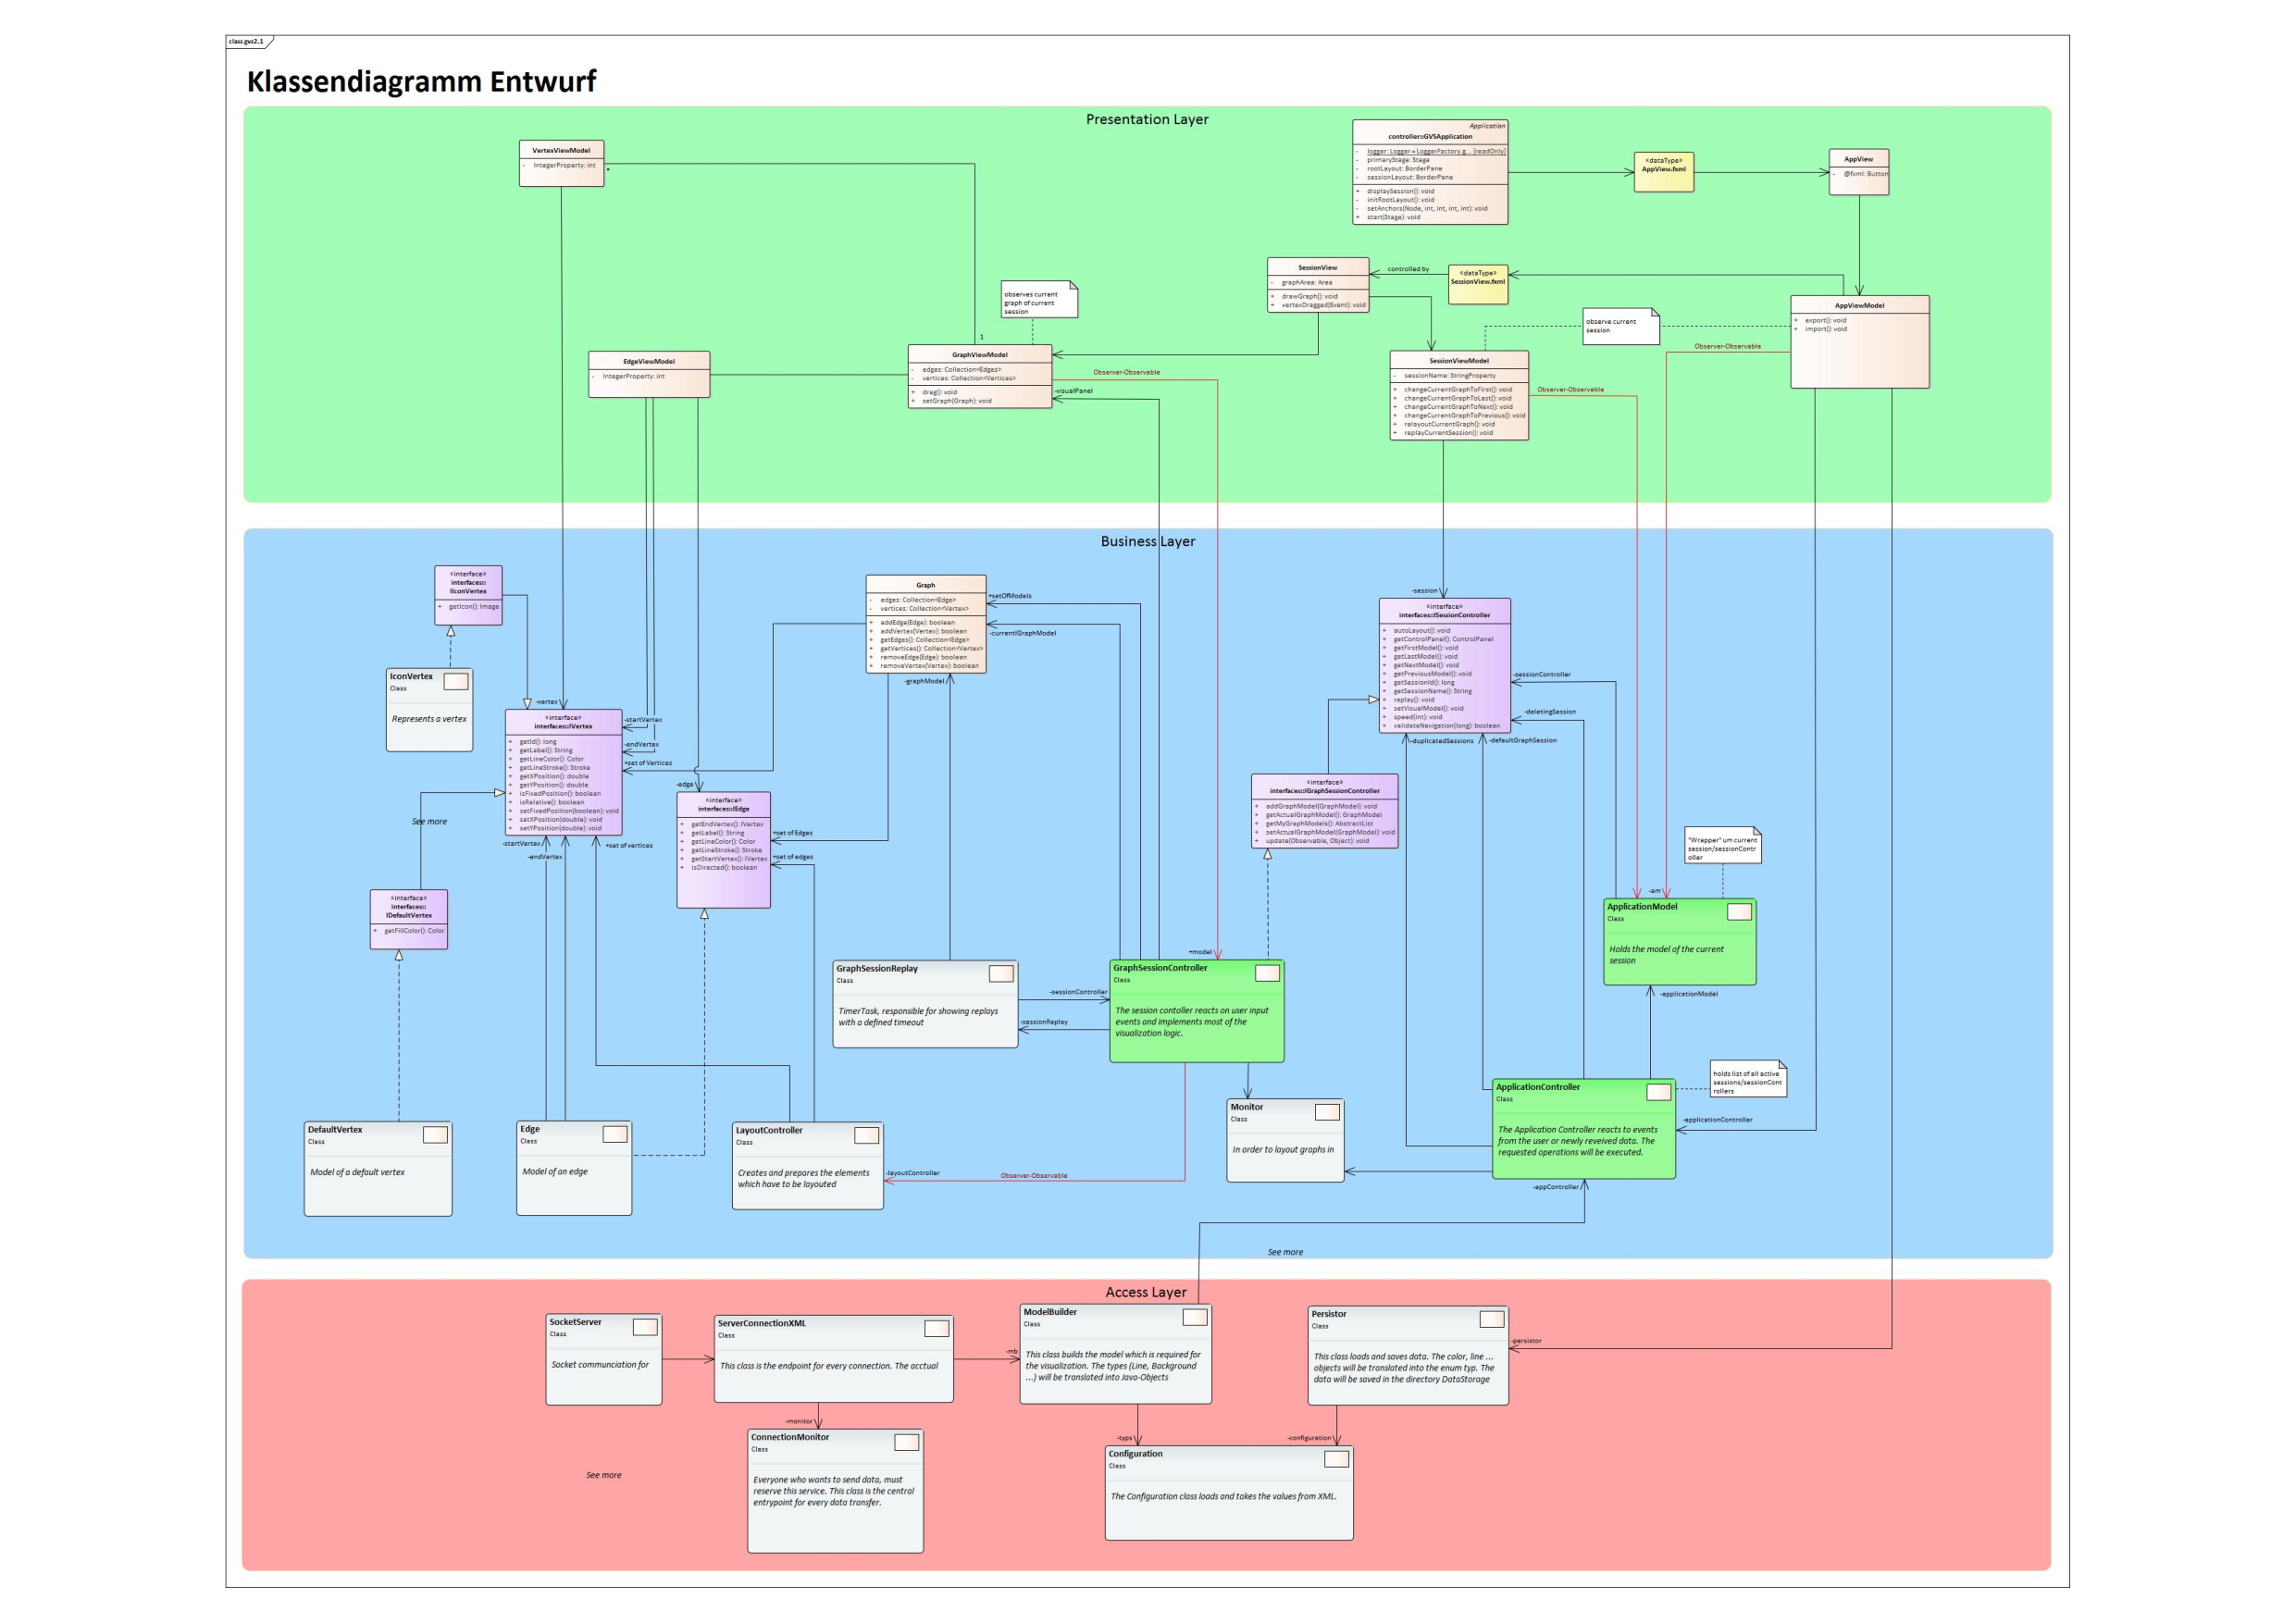
\includepdf[fitpaper]{assets/pdf/gvs2-0.pdf}
	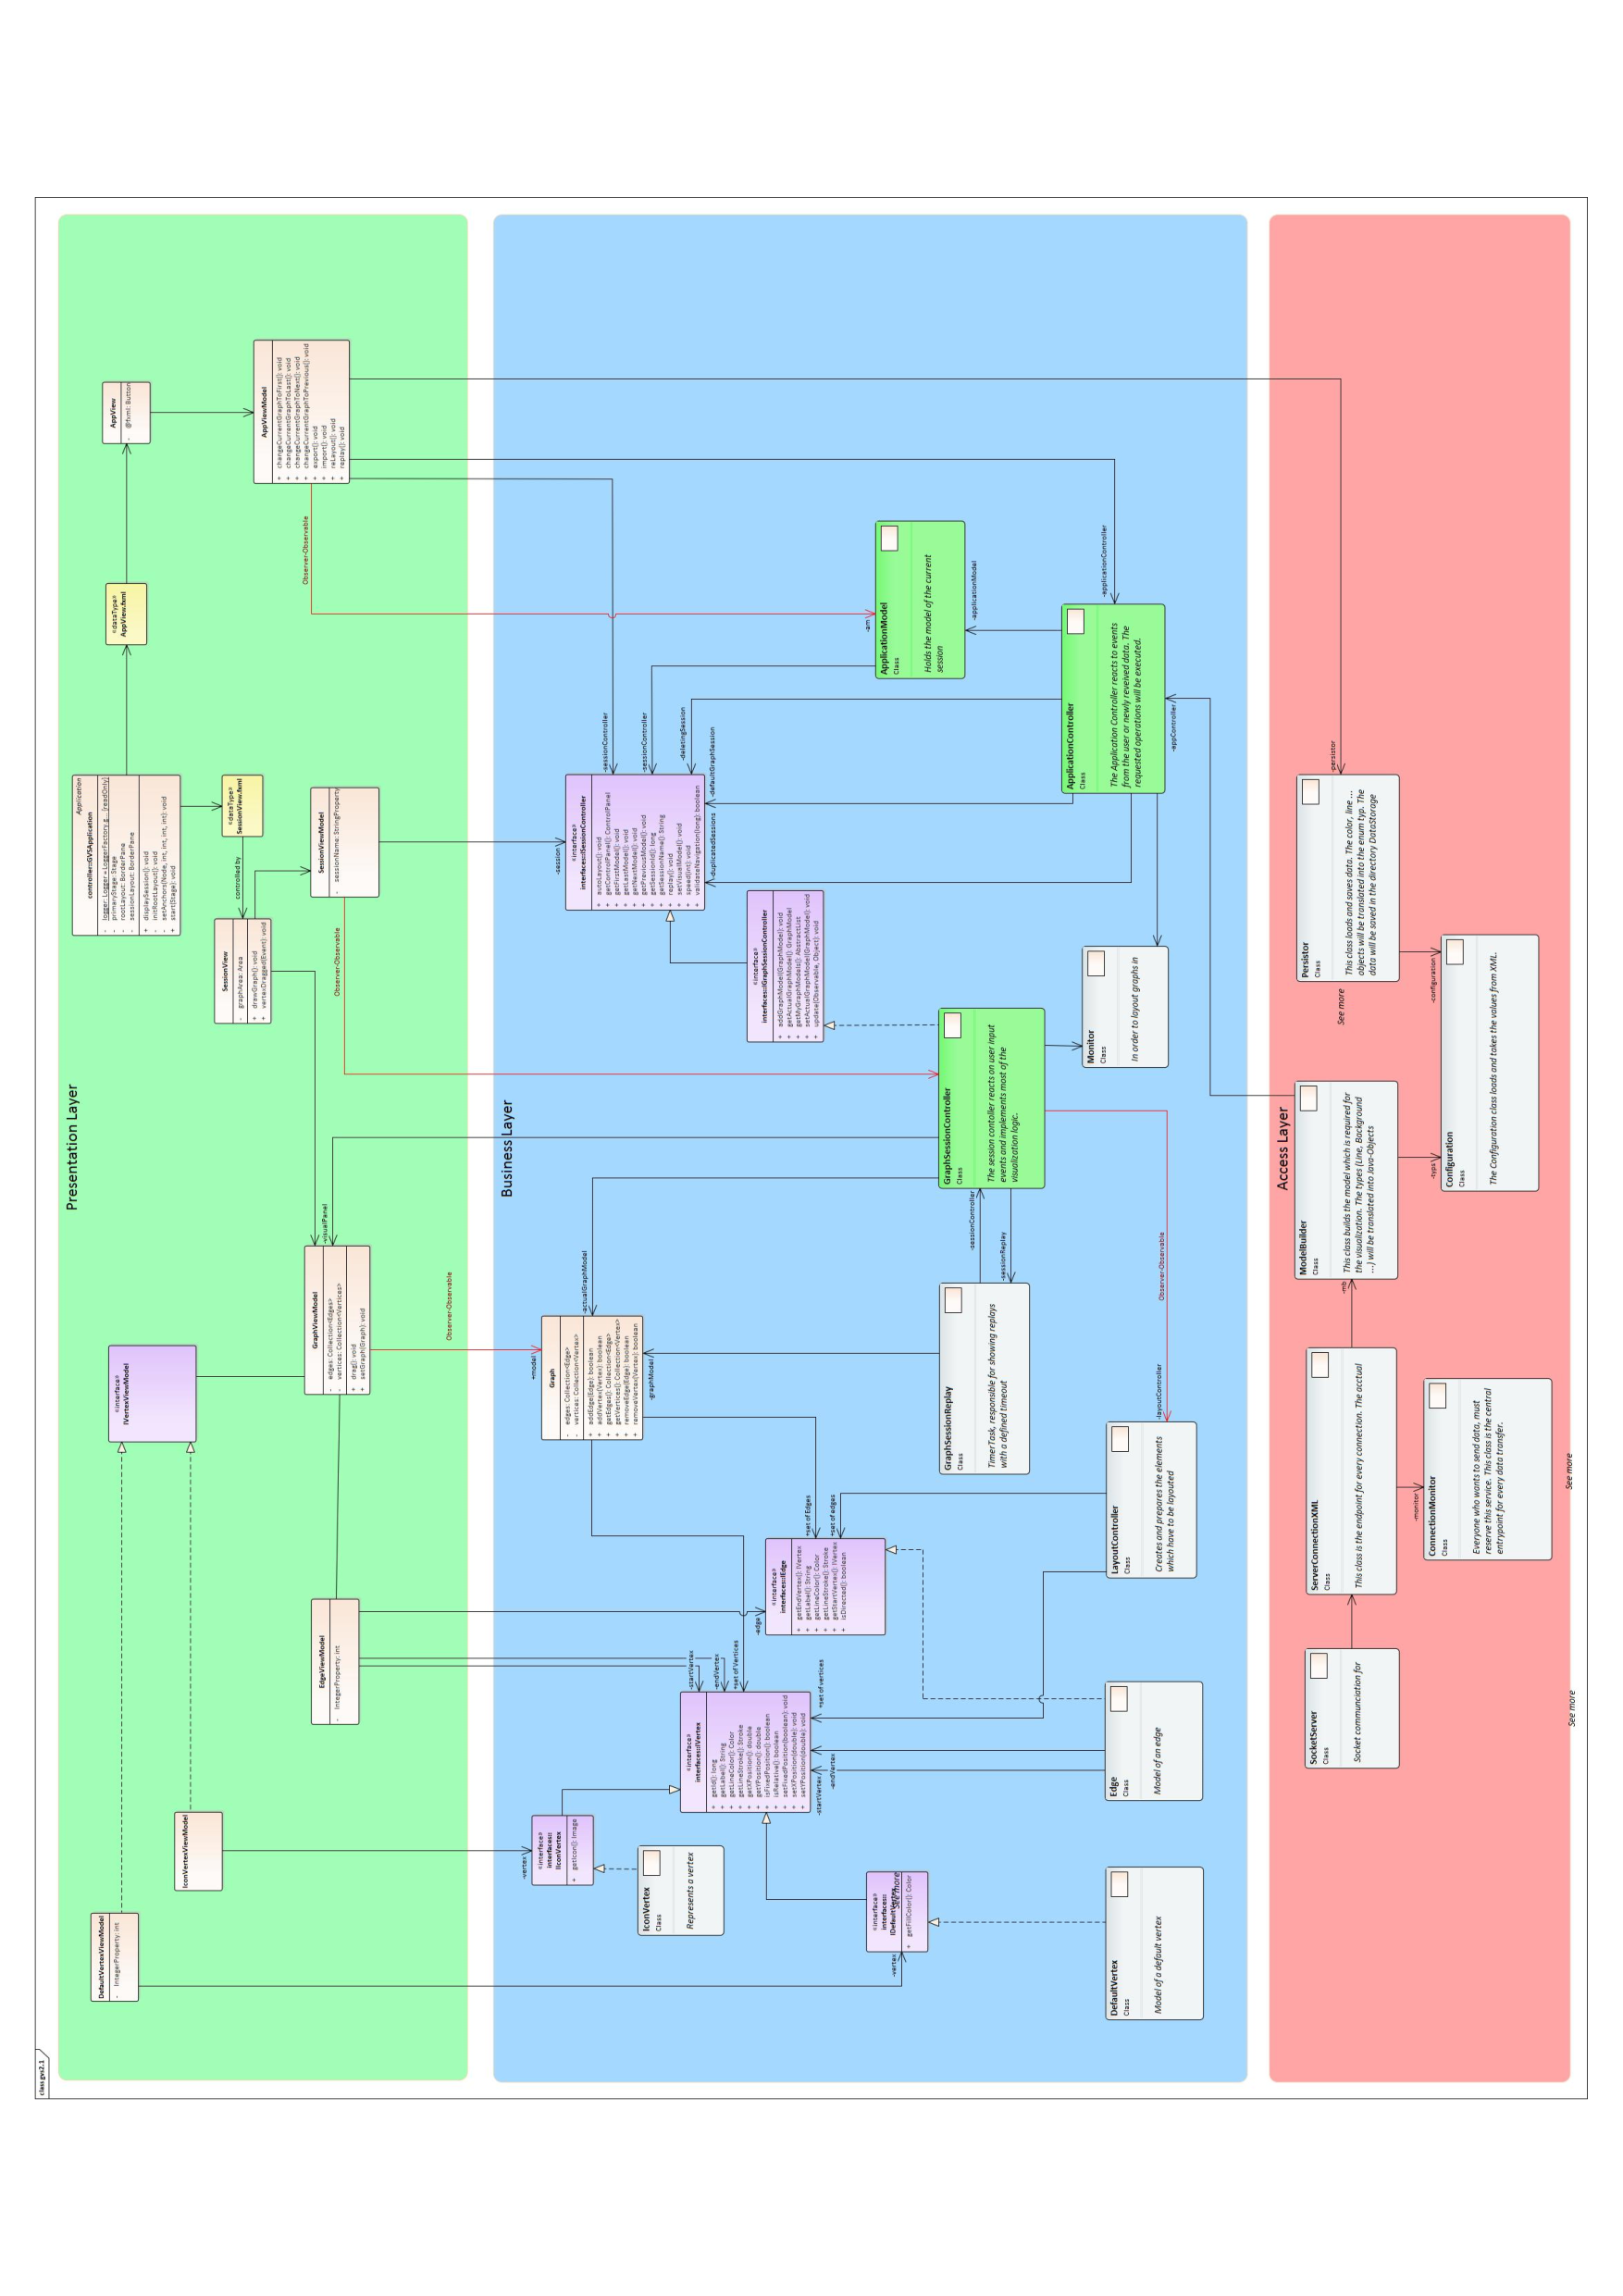
\includepdf[fitpaper]{assets/pdf/gvs2-1.pdf}
	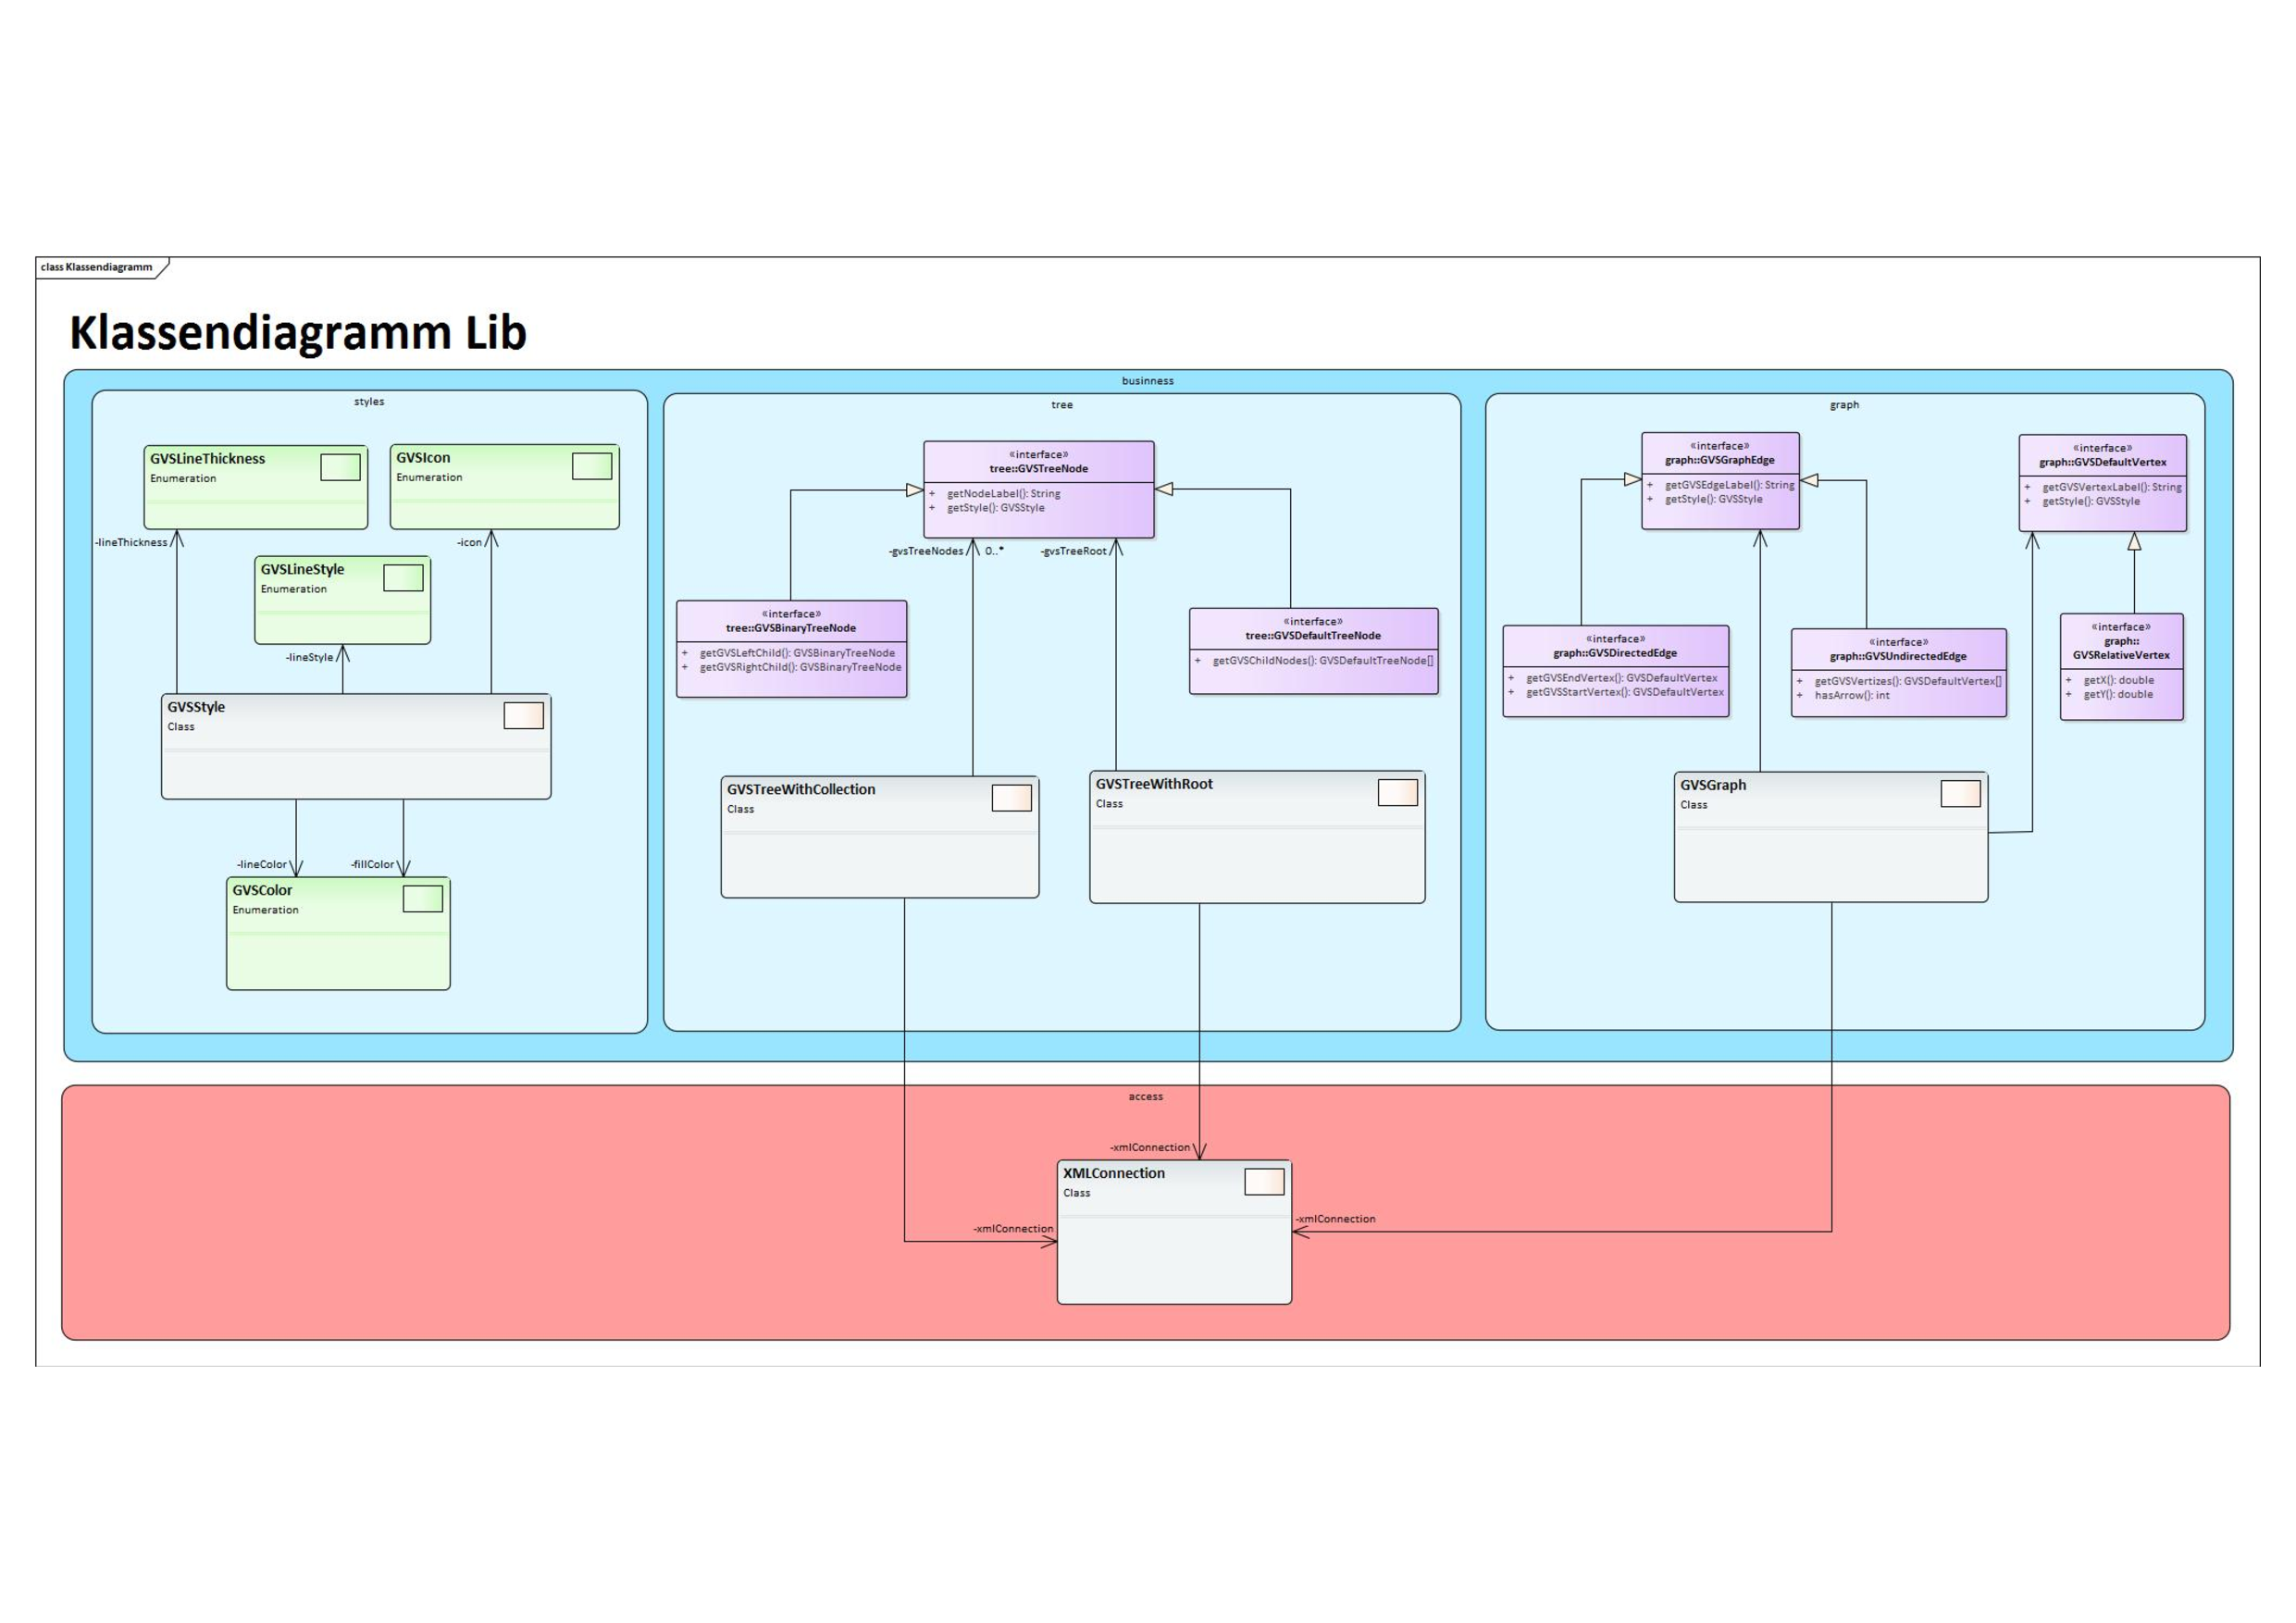
\includepdf[fitpaper]{assets/pdf/gvs2-lib.pdf}
	
	\chapter{Migrationsliste} \label{ch:migration-list}
	Die Migrationsliste gibt einen Überblick über die geplante Migration aller GVS 1.0 Klassen.
	
	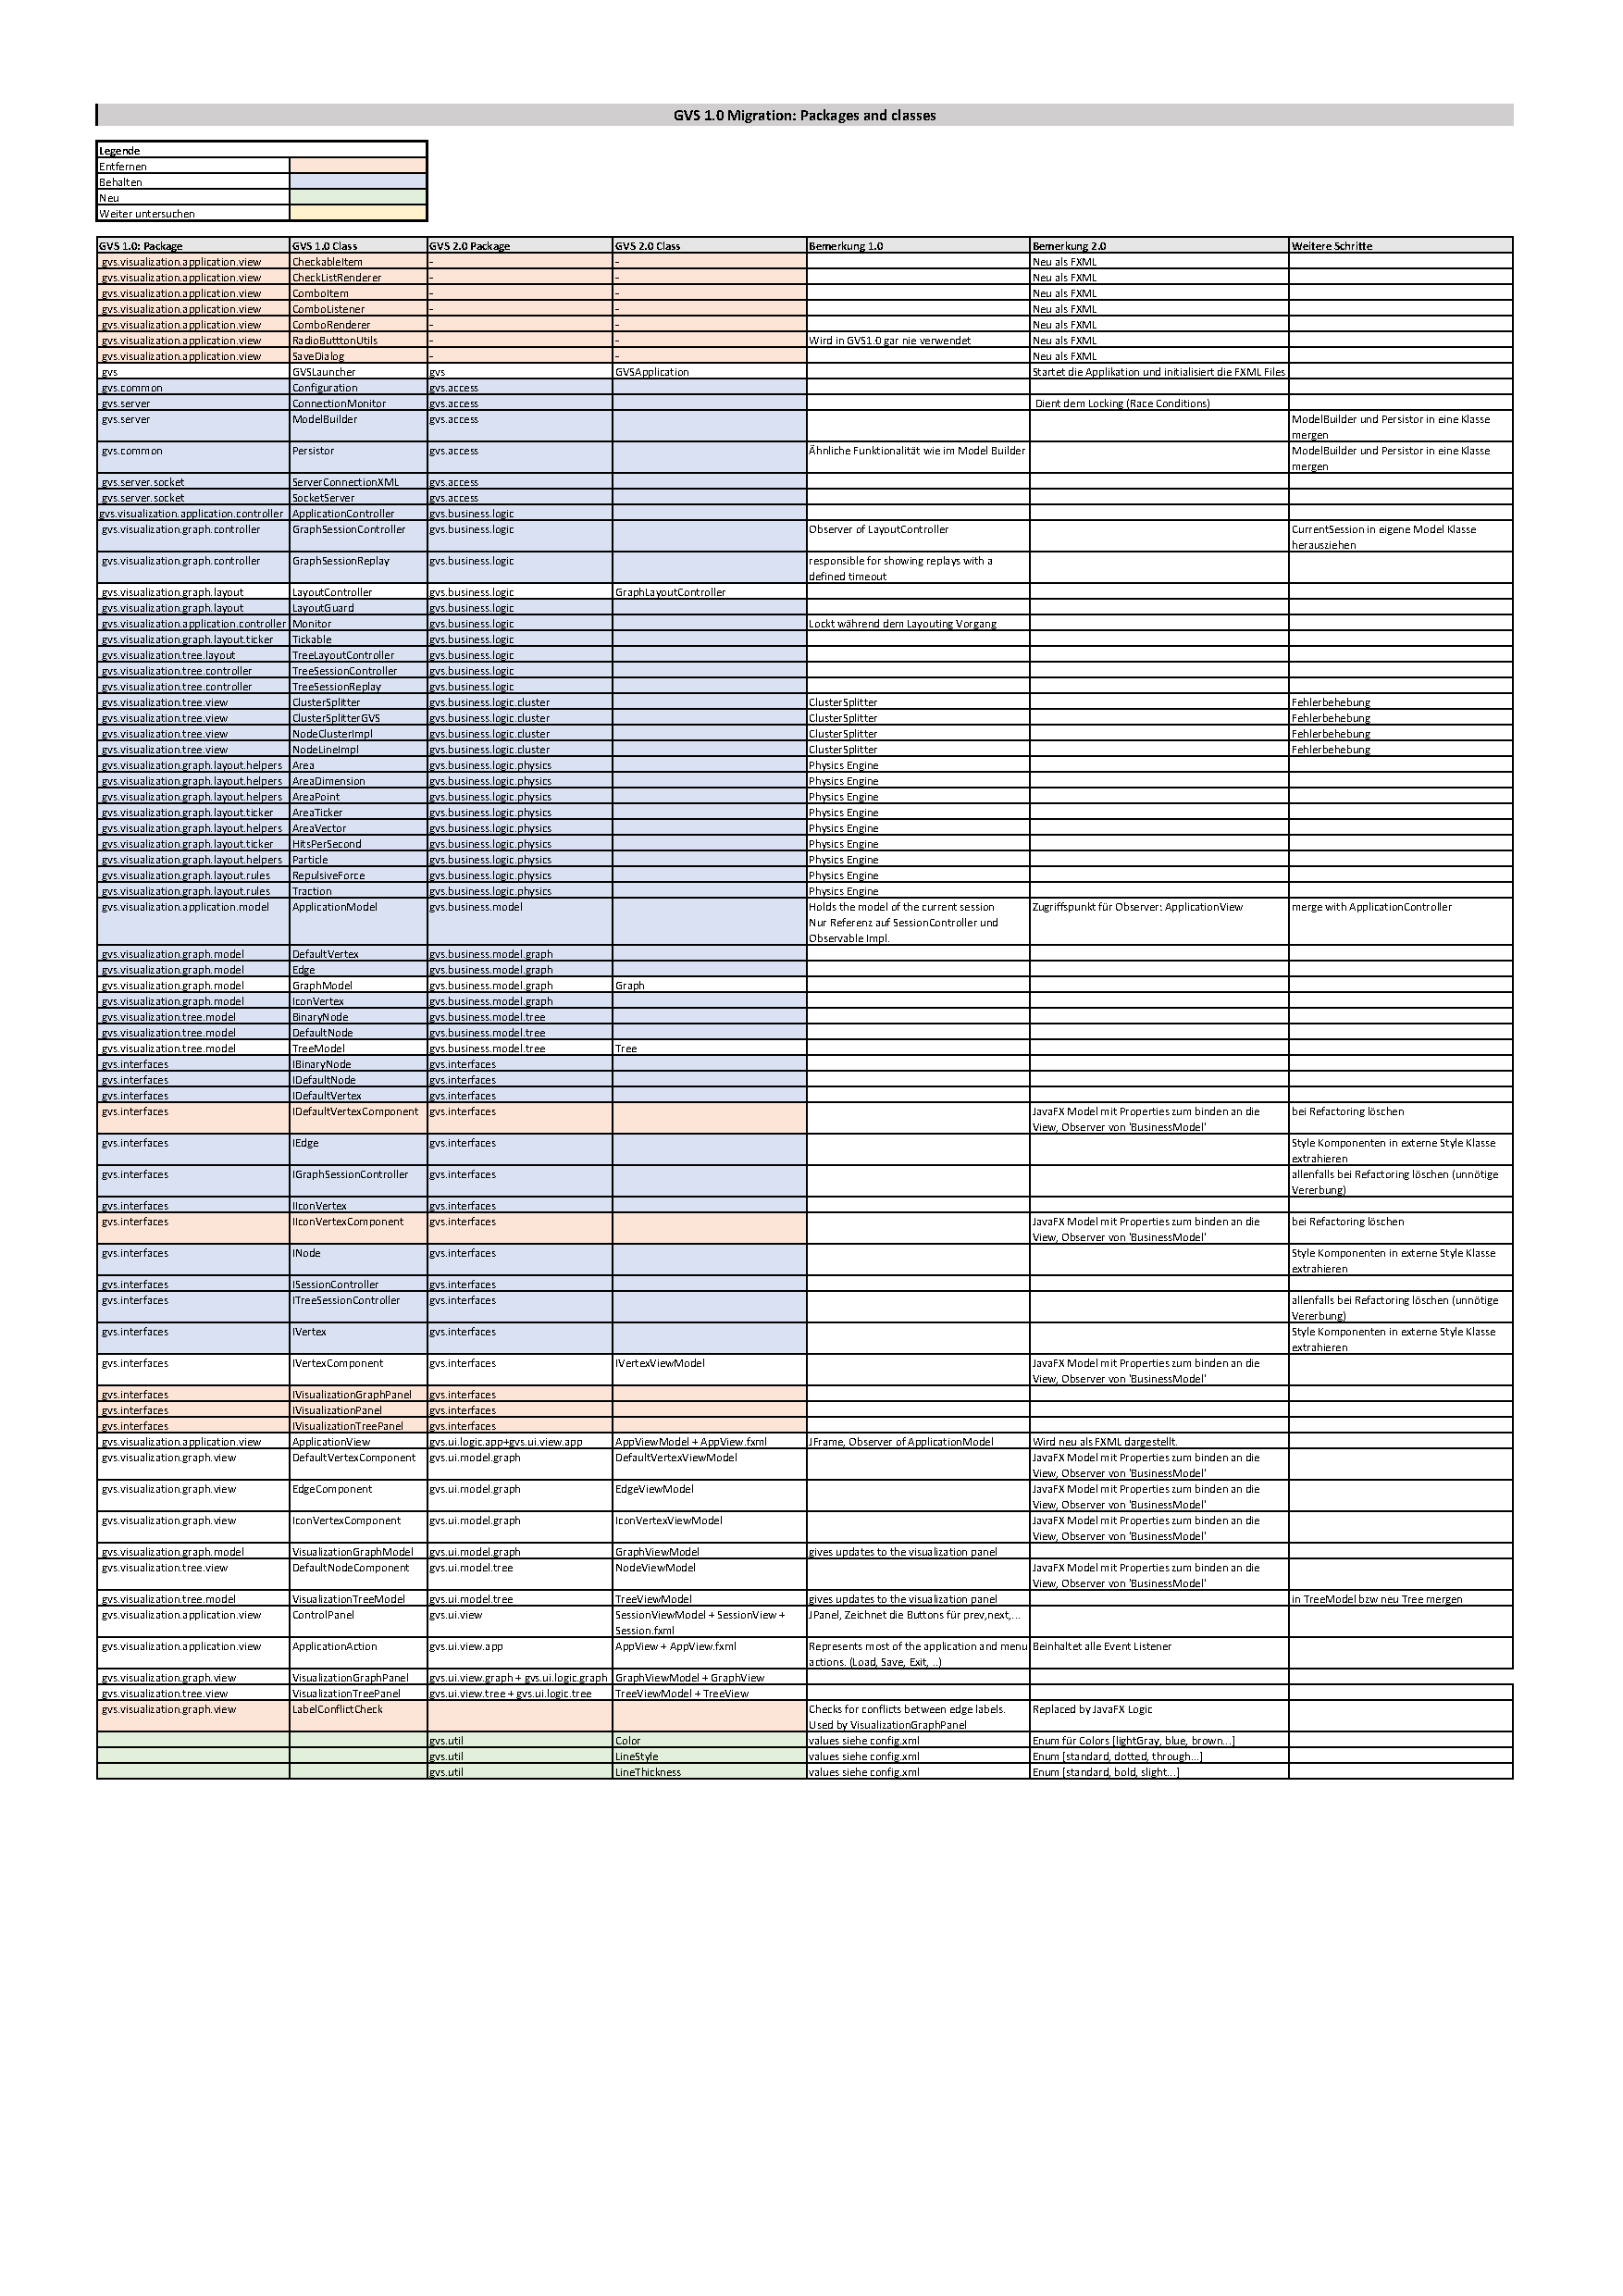
\includepdf[fitpaper]{assets/pdf/Migration_Replacements.pdf}
	
	\chapter{Aufgabenstellung}
	\label{aufgabenstellung}
	Die folgenden Seiten enthalten die offizielle Aufgabenstellung dieser Studienarbeit.
	
	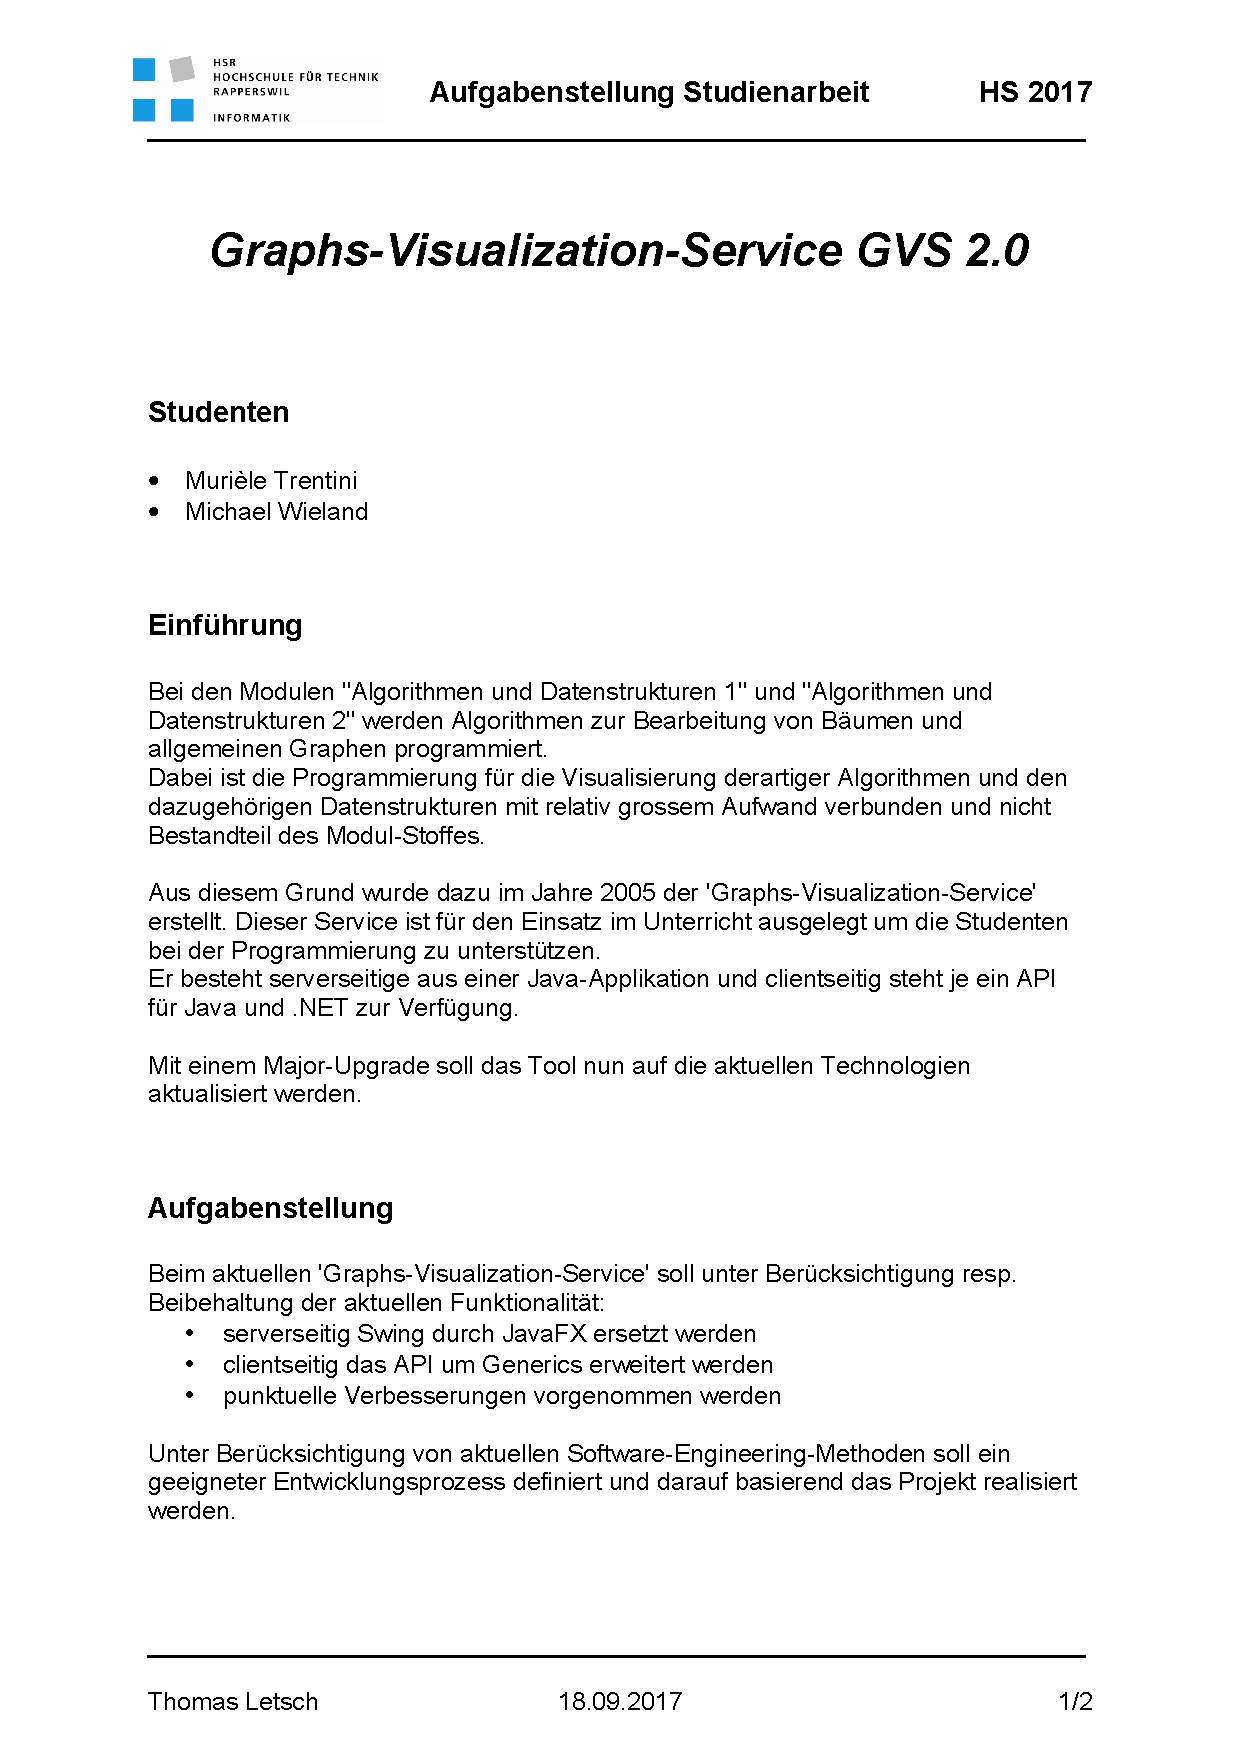
\includepdf[pages={1-}]{assets/Aufgabenstellung_GVS2.pdf}
	
	\chapter{Testprotokoll} \label{Testprotokoll}
	\section{Systemtests}
	
	\begin{enumerate}
		\item System Tests 04.12.17
		\item System Tests 15.12.17
	\end{enumerate}

	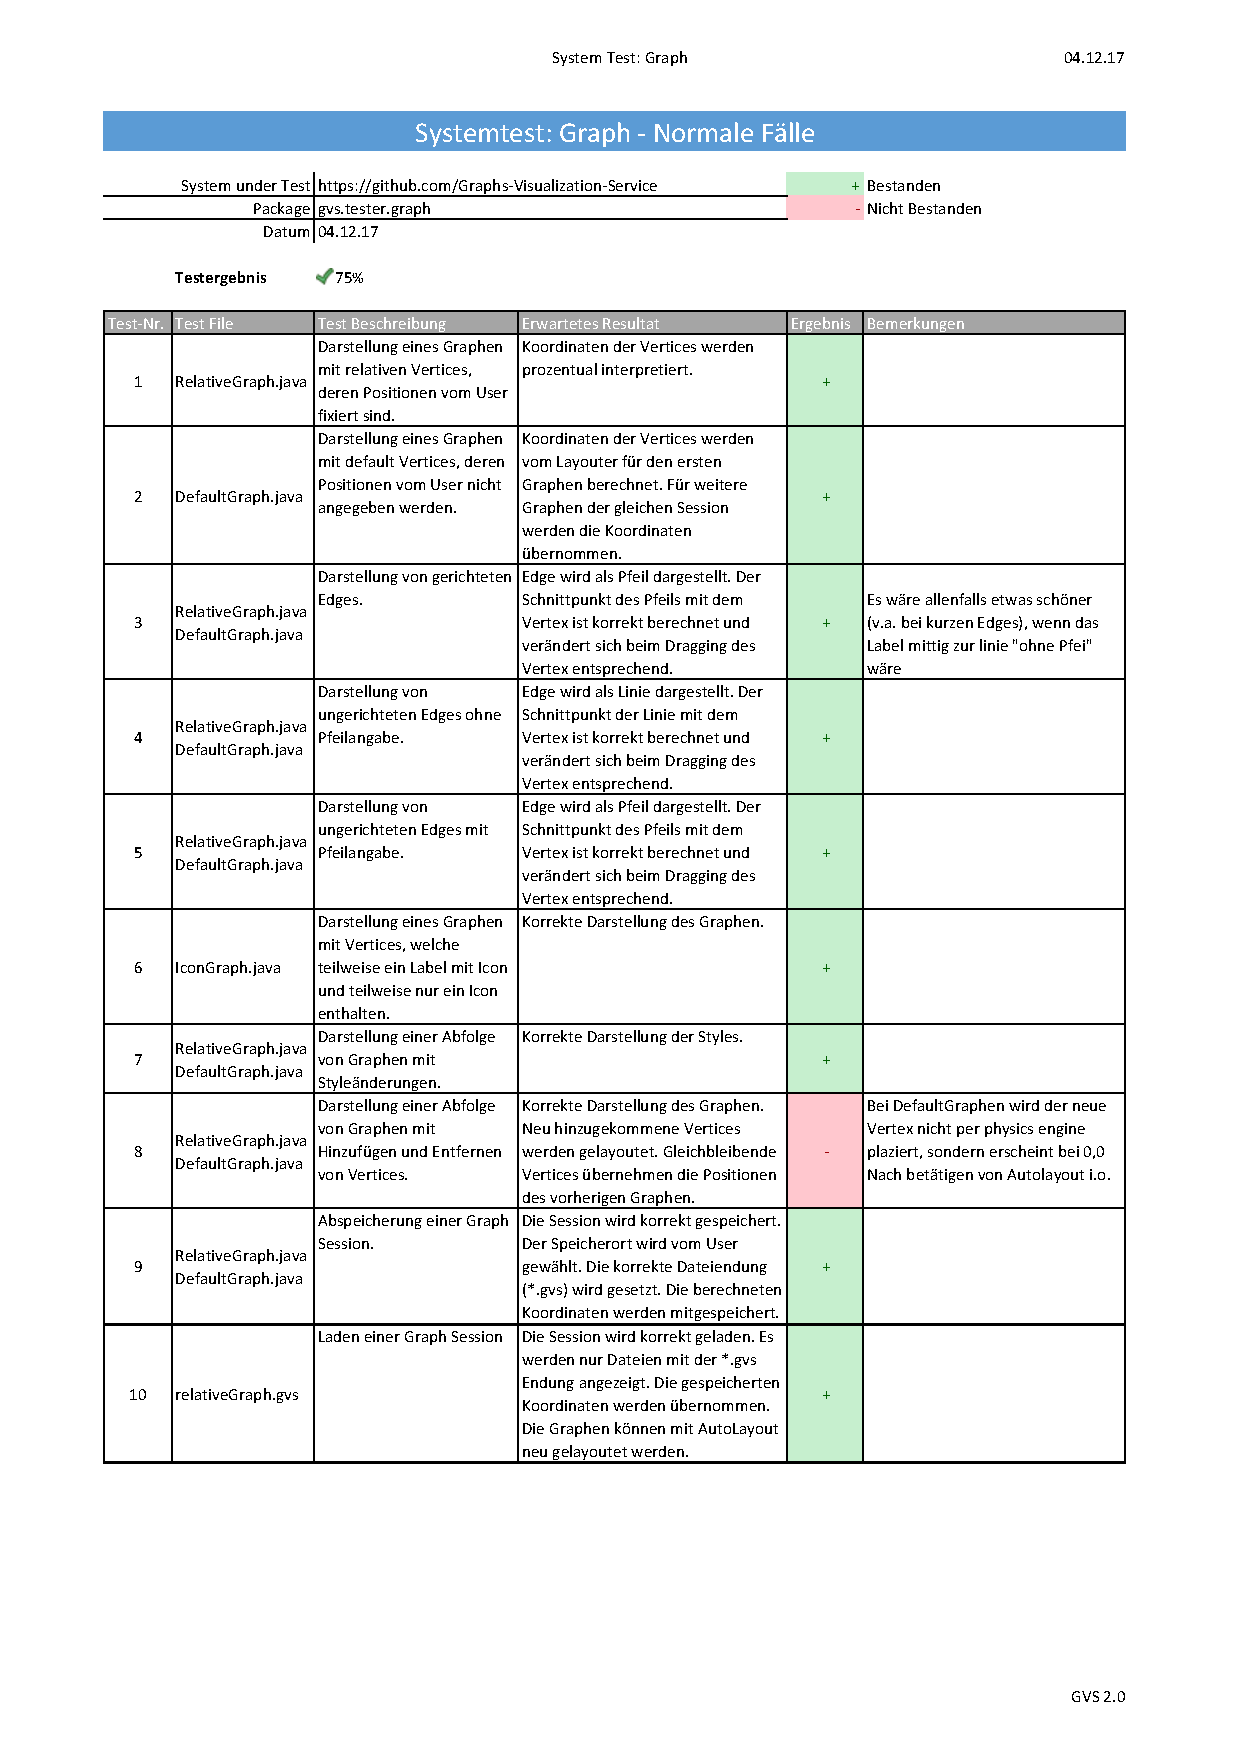
\includepdf[pages={1-}]{assets/pdf/SystemTests-17-12-04}
	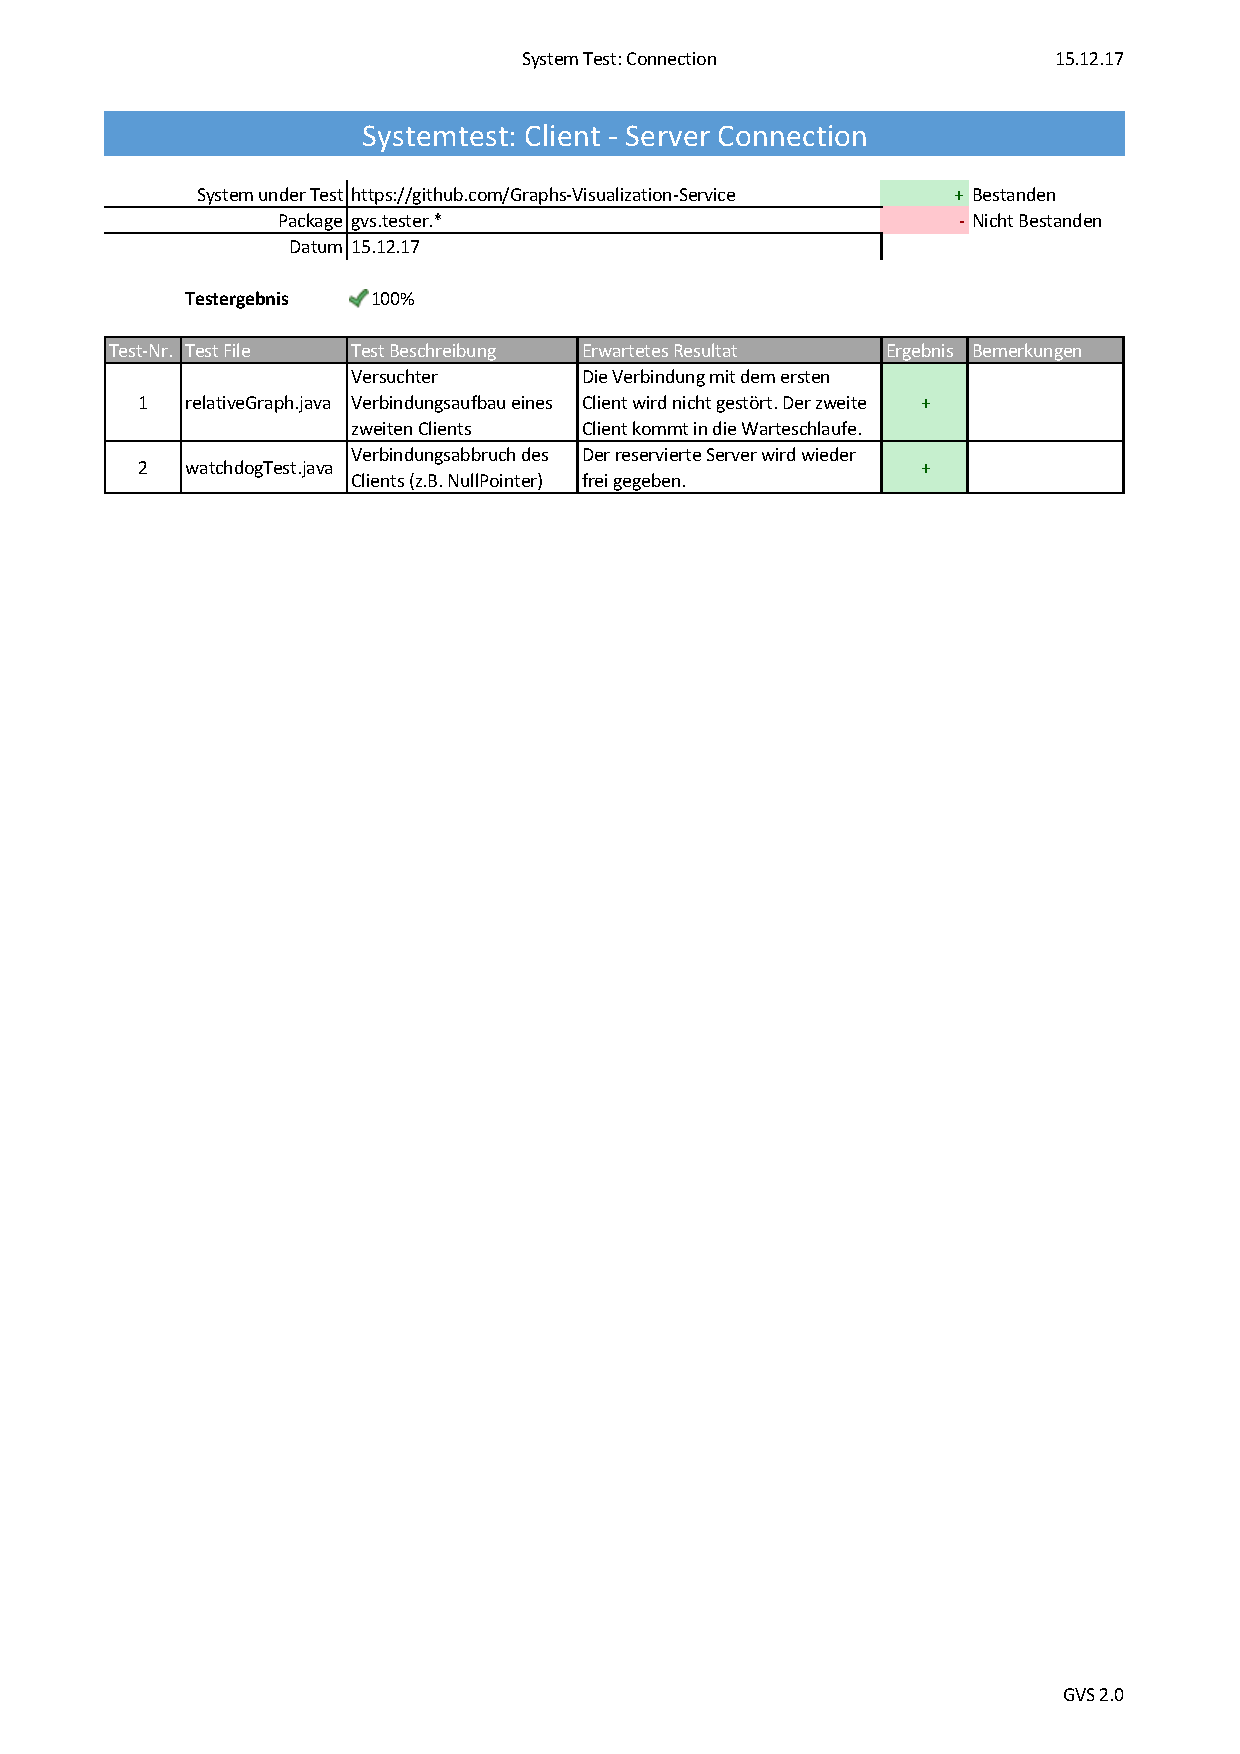
\includepdf[pages={1-}]{assets/pdf/SystemTests-17-12-15}
	
	\clearpage
	
	
	
	\section{Usability Tests}
	Viele Funktionen sind im GVS 1.0 versteckt und es ist nicht immer klar, was eine Funktion auslöst. Beim Design von GVS 2.0 wurde deshalb darauf geachtet, dass ein minimales, sprechendes UI erstellt wird. Beim Vergleich der beiden Programmfenster (siehe Abb. \ref{fig:gvs-1} und \ref{fig:gvs-2}) sind die Unterschiede gut erkennbar. 
	
	\begin{figure}[h!]
		\centering
		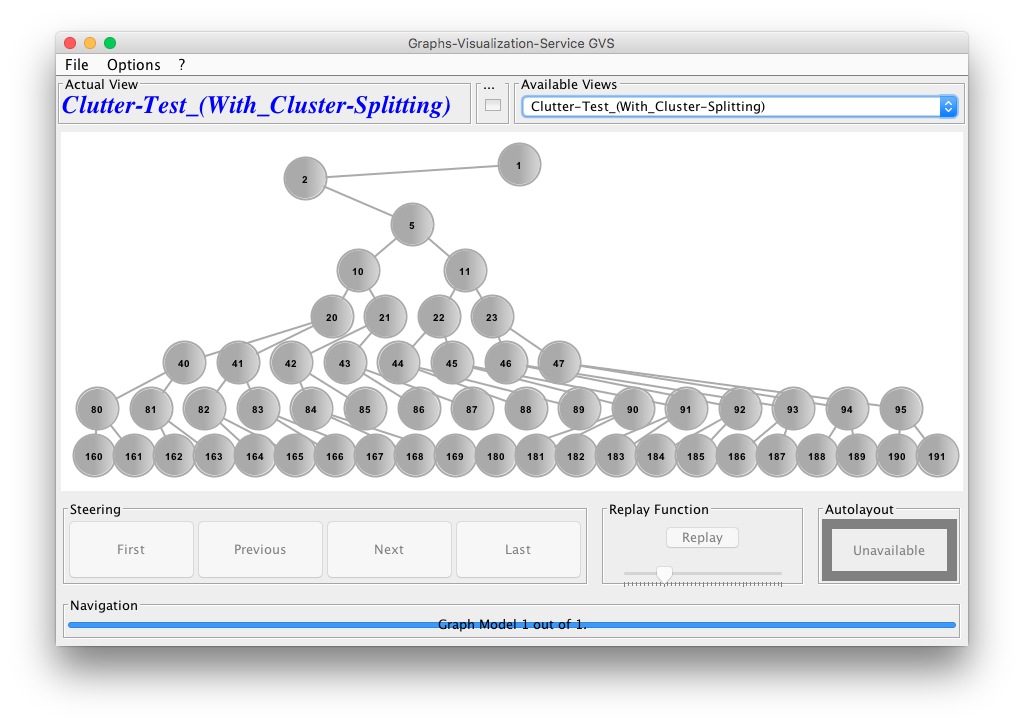
\includegraphics[width=0.6\linewidth]{assets/images/gvs-1}
		\caption{GVS 1.0: User Interface}
		\label{fig:gvs-1}
	\end{figure}

	\begin{figure}[h!]
		\centering
		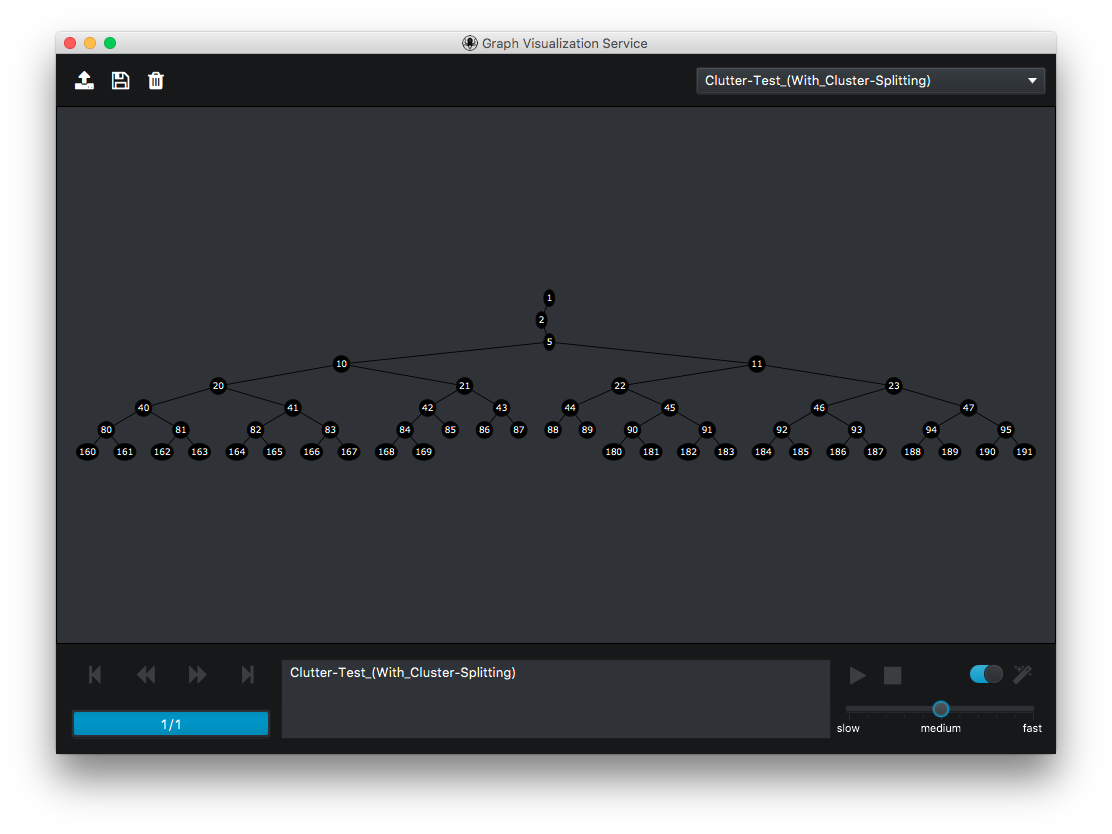
\includegraphics[width=0.6\linewidth]{assets/images/gvs-2}
		\caption{GVS 2.0: User Interface}
		\label{fig:gvs-2}
	\end{figure}
	
	\begin{table}[h!]
		\centering
		\begin{tabularx}{\linewidth}{X X }
			\toprule 
			Erkannte Mängel GVS 1.0 & Einfluss auf GVS 2.0\\
			\midrule
			Veraltetes User Interace & Modernes, ansprechendes User Interface, mit dunklen Farben, damit die Algorithmen besser farblich hervorgehoben werden \\
			Icons werden unter Unix nicht dargestellt & Moderne, sprechende \gls{fontawesome} Icons einführen. Die Icons werden auf allen Plattformen korrekt dargestellt \\
			Funktion \textit{Random und Stable Layout} ist nicht klar & Die Funktion wird wegen fehlendem praktischen Nutzen entfernt \\
			Funktion \textit{Cluster Splitter} ist nicht klar & Ein spezieller Layout Algorithmus für Binary Trees wird implementiert \\
			Beim Laden von gespeicherten Session muss der Speicherort immer wieder von Neuem ausgewählt werden & Der zuletzt verwendete Speicherort wird gespeichert \\
			Graph Vertices lassen sich ausserhalb des sichtbaren Programmfenster draggen & ZoomPane skaliert das Fenster, sobald ein Knoten den Viewport verlässt \\
			Autolayout Funktion ist nur für die letzten Momentaufnahme eines Graphen möglich & Die Autolayout Funktion ist für alle Momentaufnahmen möglich \\
			Drag Support ist nur für die letzte Momentaufnahme eines Graphen möglich & Dragging von Vertices ist immer möglich \\
			Koordinaten von gedraggten Vertices werden nicht für die nächste Momentaufnahme übernommen & Koordinaten werden immer übernommen \\
			\textit{Replay} Geschwindigkeit wird in Millisekunden dargestellt & Es gibt nur doch die drei Geschwindigkeiten \textit{langsam}, \textit{normal} und \textit{schnell} \\
			Server Applikation wird beim Absturz des Client nicht freigegeben & Watchdog Service gibt den Server bei inaktiven Clients wieder frei \\
			\bottomrule 
		\end{tabularx} 
		\caption{Usability Tests} 
	\end{table}
	
	\chapter{Persönliche Berichte}
	\label{erfahrungsberichte}
	\section{Murièle Trenini}
	
	Meine bisherige Erfahrung mit Informatik Projekten beschränkt sich auf das Engineering Projekt aus dem vergangenen Semester. Im Kontrast dazu stand vor allem, dass dieses Projekt nicht ''auf der grünen Wiese'' stattfand. Für mich war der Umgang mit Legacy Code eine neue Erfahrung, die interessant aber auch herausfordernd war. Zu Beginn des Projektes, aber auch während der Refactoring Phase, war viel Zeit nötig, um bestehenden Code und bisherige Programmabläufe nachzuvollziehen.  \\

	\noindent	
	Wir haben uns voller Elan daran gemacht, den bestehenden Code unseren Achitektur- und Qualitätsansprüchen anzupassen. Leider litt die Funktionalität teilweise darunter. So kam es vor, dass Code Abschnitte im Zuge eines Refactorings weg rationalisiert wurden, nur um später festzustellen, dass der Abschnitt wieder Erwartens notwendig war. Für zukünftige Projekte nehme ich mir vor, Code Abschnitte in Legacy Code genau zu hinterfragen, bevor sie umgeschrieben oder gelöscht werden. Hier hätte sicher auch eine bessere Testabdeckung geholfen. Leider ist es auch uns nicht gelungen, grössere Teile der Applikation mit automatisierten Tests abzudecken. \\

	\noindent	
	Die gute Zusammenarbeit mit meinem Projektpartner, Michael Wieland, habe ich geschätzt und sie hat mich immer wieder motiviert, selber eben soviel Einsatz zu geben um ein qualitativ hochwertiges Endresultat zu erreichen. Ich freue mich auf die nächste Herausforderung, welche wir in der Bachelorarbeit gemeinsam bestreiten werden.\\
	
	\noindent
	Mit dem Endresultat bin ich sehr zufrieden.  Ich denke wir dürfen stolz sein über die Qualität des Codes, welche wir im Laufe dieses Projektes ständig erhöhen konnten. Dies zeigt sich auch deutlich in den verwendeten Metriken. Optisch finde ich GVS 2.0 sehr ansprechend und ich bin mir sicher, dass es die Verbesserung der Usability (u.A. durch die Einführung des Watchdogs) zukünftigen Studenten erleichtert, mit der Applikation umzugehen.
	
	\clearpage
	\section{Michael Wieland}
	Die Durchführung unserer Studienarbeit war durchgehend spannend, da wir uns stets neuen Herausforderungen stellen durften. Den Anfang machte die Analyse des bestehenden Codes. Dieser war sichtlich in die Jahre gekommen und schien (wahrscheinlich aus Zeitgründen) viel Code Duplikate zu enthalten. Dies machte es schwierig, das Wesentliche herauszufiltern. So war es nicht erstaunlich, dass wir von dem geplanten Vorgehen, möglichst viel Code wiederzuverwenden, schon bald abweichen mussten. In der Analyse Phase war es dann interessant, die Architektur so zu planen, wie es in diversen Modulen der HSR vermittelt wird. Unter anderem in interessanten Gesprächen mit Prof. Olaf Zimmermann konnte eine flexible Architektur designed werden, die es auch Folgearbeiten erleichtern wird, Erweiterungen anzubringen. \\
	
	\noindent
	Der Zeitaufwand für das Projekt war relativ gross. Zu Beginn des Projekts konnte man annehmen, dass man durch die bereits existierende Lösung viel Zeit einsparen kann. Es zeichnete sich aber ab, dass für das Verständnis des existierenden Code etwa gleich viel Zeit aufgewendet werden musste, wie für den Neuentwurf der Funktionalität. So mussten schlussendlich auch in diesem Projekt einige Abstriche zugunsten der Zeit gemacht werden. Ich bin aber überzeugt, dass die aktuelle Architektur wesentlich verständlicher wie die Alte ist. \\
	
	\noindent
	Die Zusammenarbeit mit Murièle war über die gesamte Projektdauer äusserst angenehm. Die Arbeitsteilung hat gut geklappt und durch die enge Zusammenarbeit und das gegenseitige Aushelfen, konnten Probleme bereits früh aus dem Weg geräumt werden. \\
	
	\noindent
	Abschliessend ist es erfreulich, dass durch diese Studienarbeit ein funktionsfähiges Produkt entstanden ist, welches den Lernerfolg zukünftiger Studenten vereinfachen wird. Nichtzugletzt wegen dem Praktischen Nutzen der Software, freue ich mich bereits jetzt auf ein interessantes Folgeprojekt im nächsten Semester.
	
	\chapter{Zeitauswertung}	\label{zeitauswertung}
	
	\section{Auswertung nach Teammitgliedern}
	\begin{figure}[h!]
		\centering
		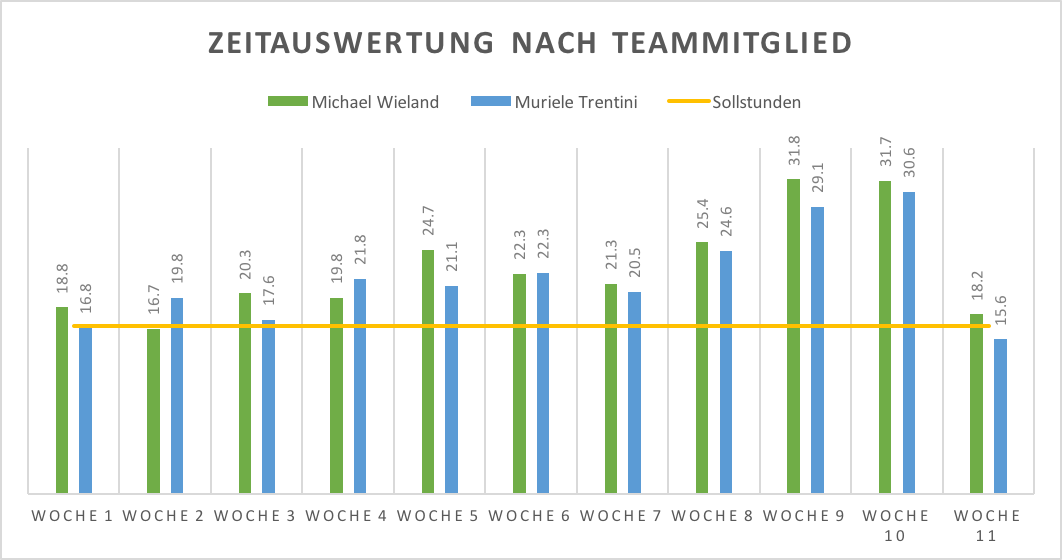
\includegraphics[width=\linewidth]{assets/images/zeitauswertung-team}
		\caption{Zeitauswertung Teammitglieder}
		\label{zeitauswertung-team}
	\end{figure}
	
	\section{Auswertung nach Kategorien}
	\begin{description}
		\item[Administratives] \hfill \\ 
		Meetings mit dem Betreuer, Sprint-Meetings, Verfassung von Protokollen, Aufsetzen der Entwicklungsumgebung \& Projektmanagement Software, Software Releases
		\item[Dokumentation] \hfill \\ 
		Verfassen der Dokumentation, Durchführen von End-to-End Tests
		\item[Implementierung] \hfill \\ 
		Schreiben von Code, inkl. Refactorings \& Unit Tests
		\item[Requirement Analyse] \hfill \\ 
		Analyse des bestehenden Legacy Codes
	\end{description}
	\begin{figure}[h!]
		\centering
		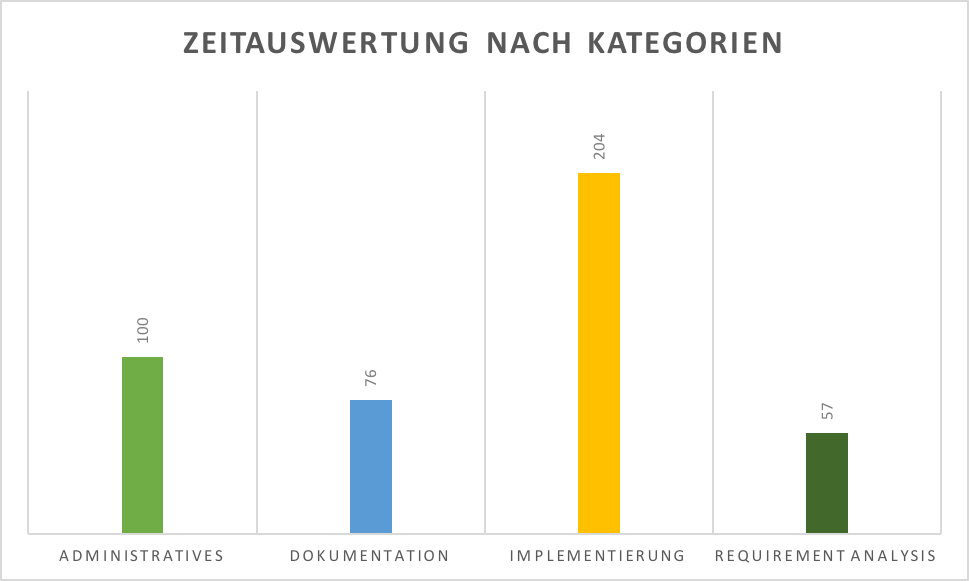
\includegraphics[width=\linewidth]{assets/images/zeitauswertung-kat}
		\caption{Zeitauswertung Kategorien Säulendiagramm}
		\label{zeitauswertung-kategorien}
	\end{figure}
	
	\clearpage

	\begin{figure}[h!]
		\centering
		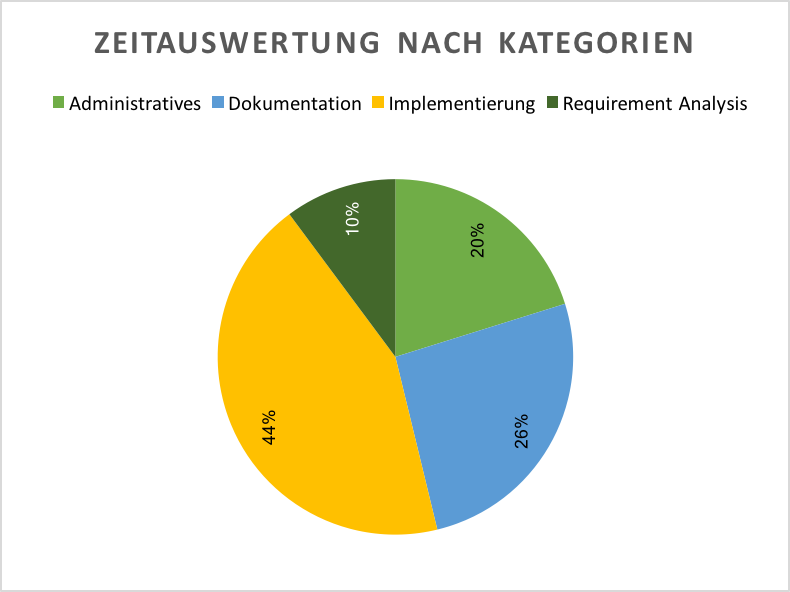
\includegraphics[width=0.7\linewidth]{assets/images/zeitauswertung-kat-pie}
		\caption{Zeitauswertung Kategorien Kuchendiagramm}
		\label{zeitauswertung-kategorien-pie}
	\end{figure}


	\section{Auswertung Soll - Ist Zeit}
	\begin{figure}[h!]
		\centering
		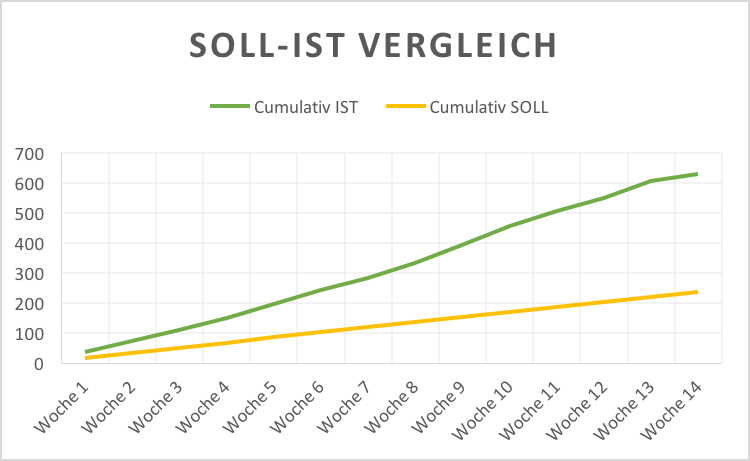
\includegraphics[width=0.7\linewidth]{assets/images/zeitauswertung-soll_ist}
		\caption{Zeitauswertung Soll - Ist Zeit}
		\label{zeitauswertung-soll_ist}
	\end{figure}
	
	\chapter{Benutzerhandbuch} \label{ch:manual}
	Nachfolgend findet sich das Benutzerhandbuch für GVS 2.0 inklusive einer Installationsanleitung für User der Library sowie für Entwickler.
	
	\includepdf[pages={1-}]{manual/Benutzerhandbuch}	
	
	\chapter{Meeting Protokolle} \label{ch:minutes}
	Nachfolgend befinden sich sämtliche Protokolle der wöchentlichen Meetings zwischen dem Betreuer und dem Projektteam.
	
	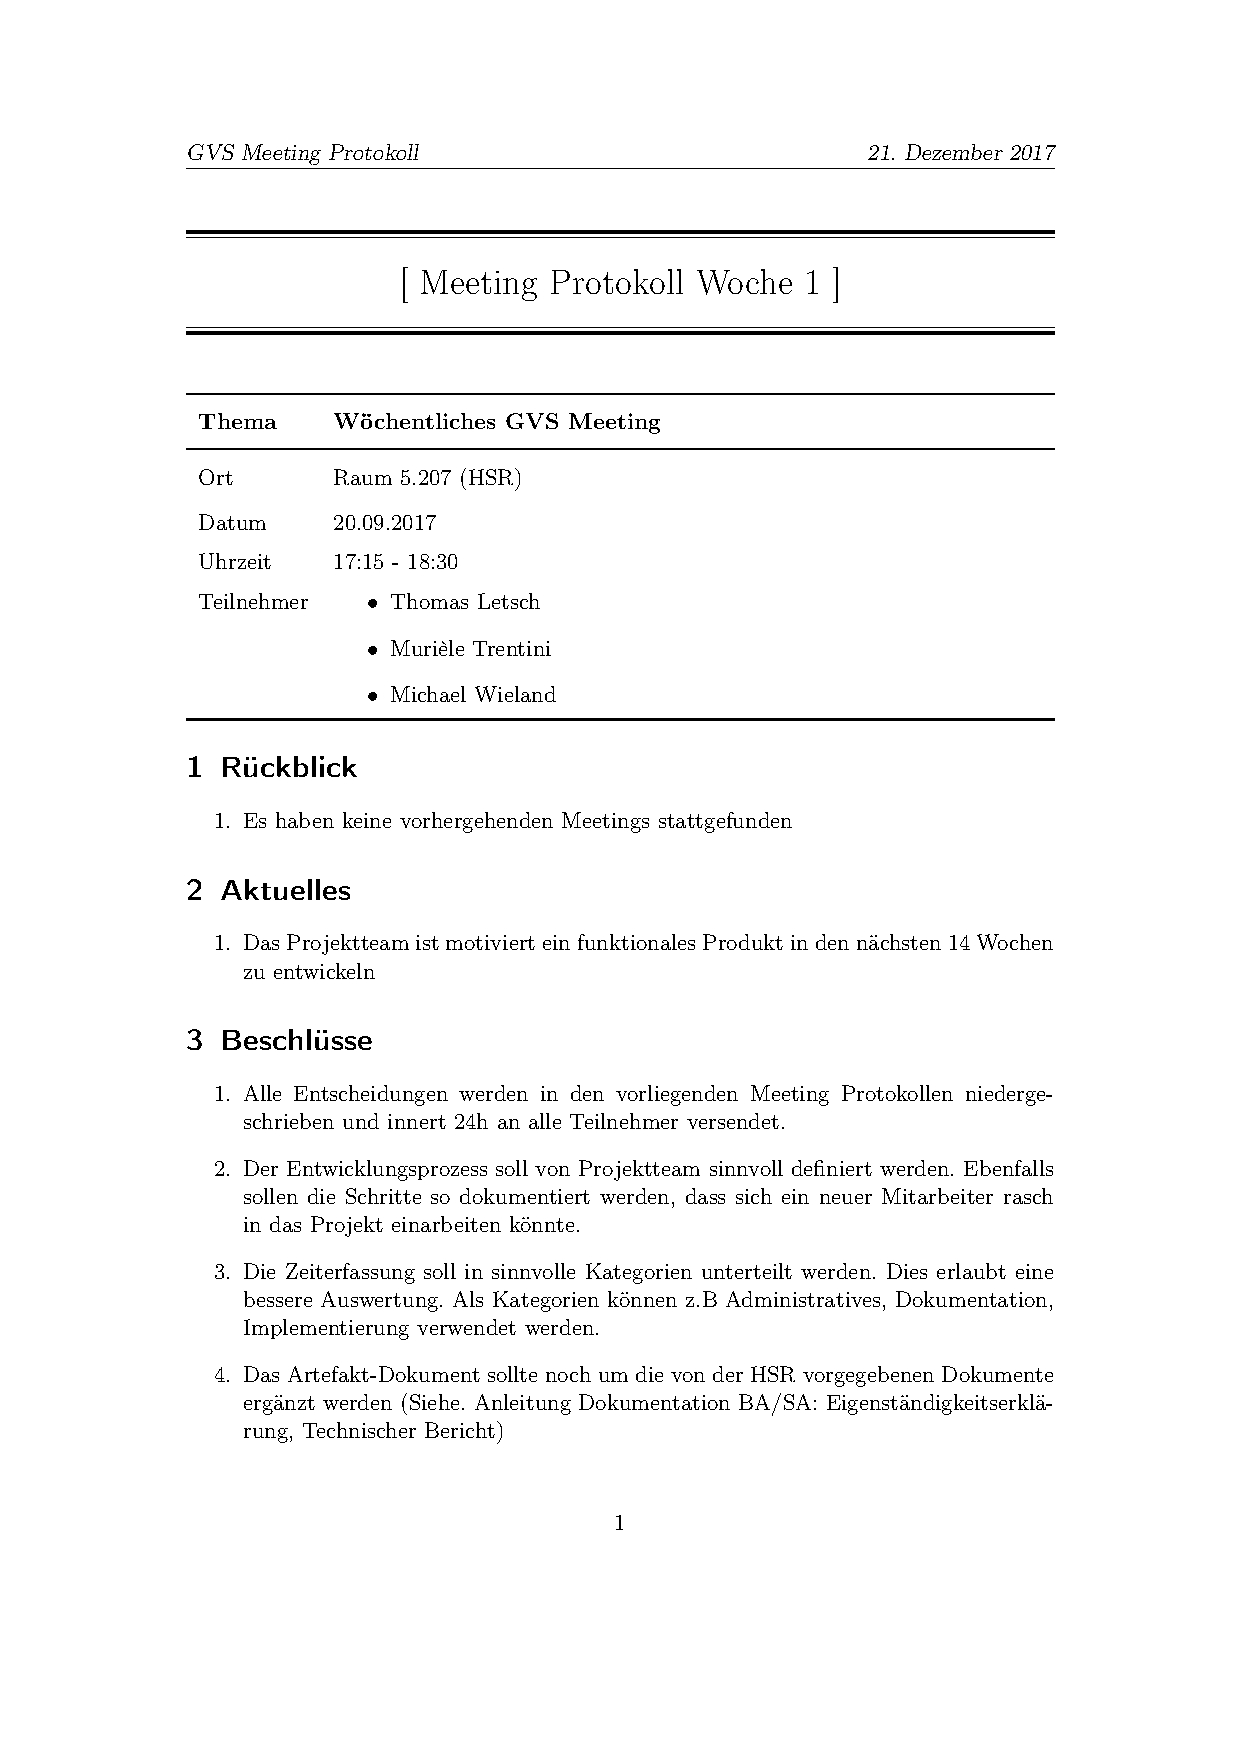
\includepdf[pages={1-}]{assets/minutes/2017-09-20.pdf}
	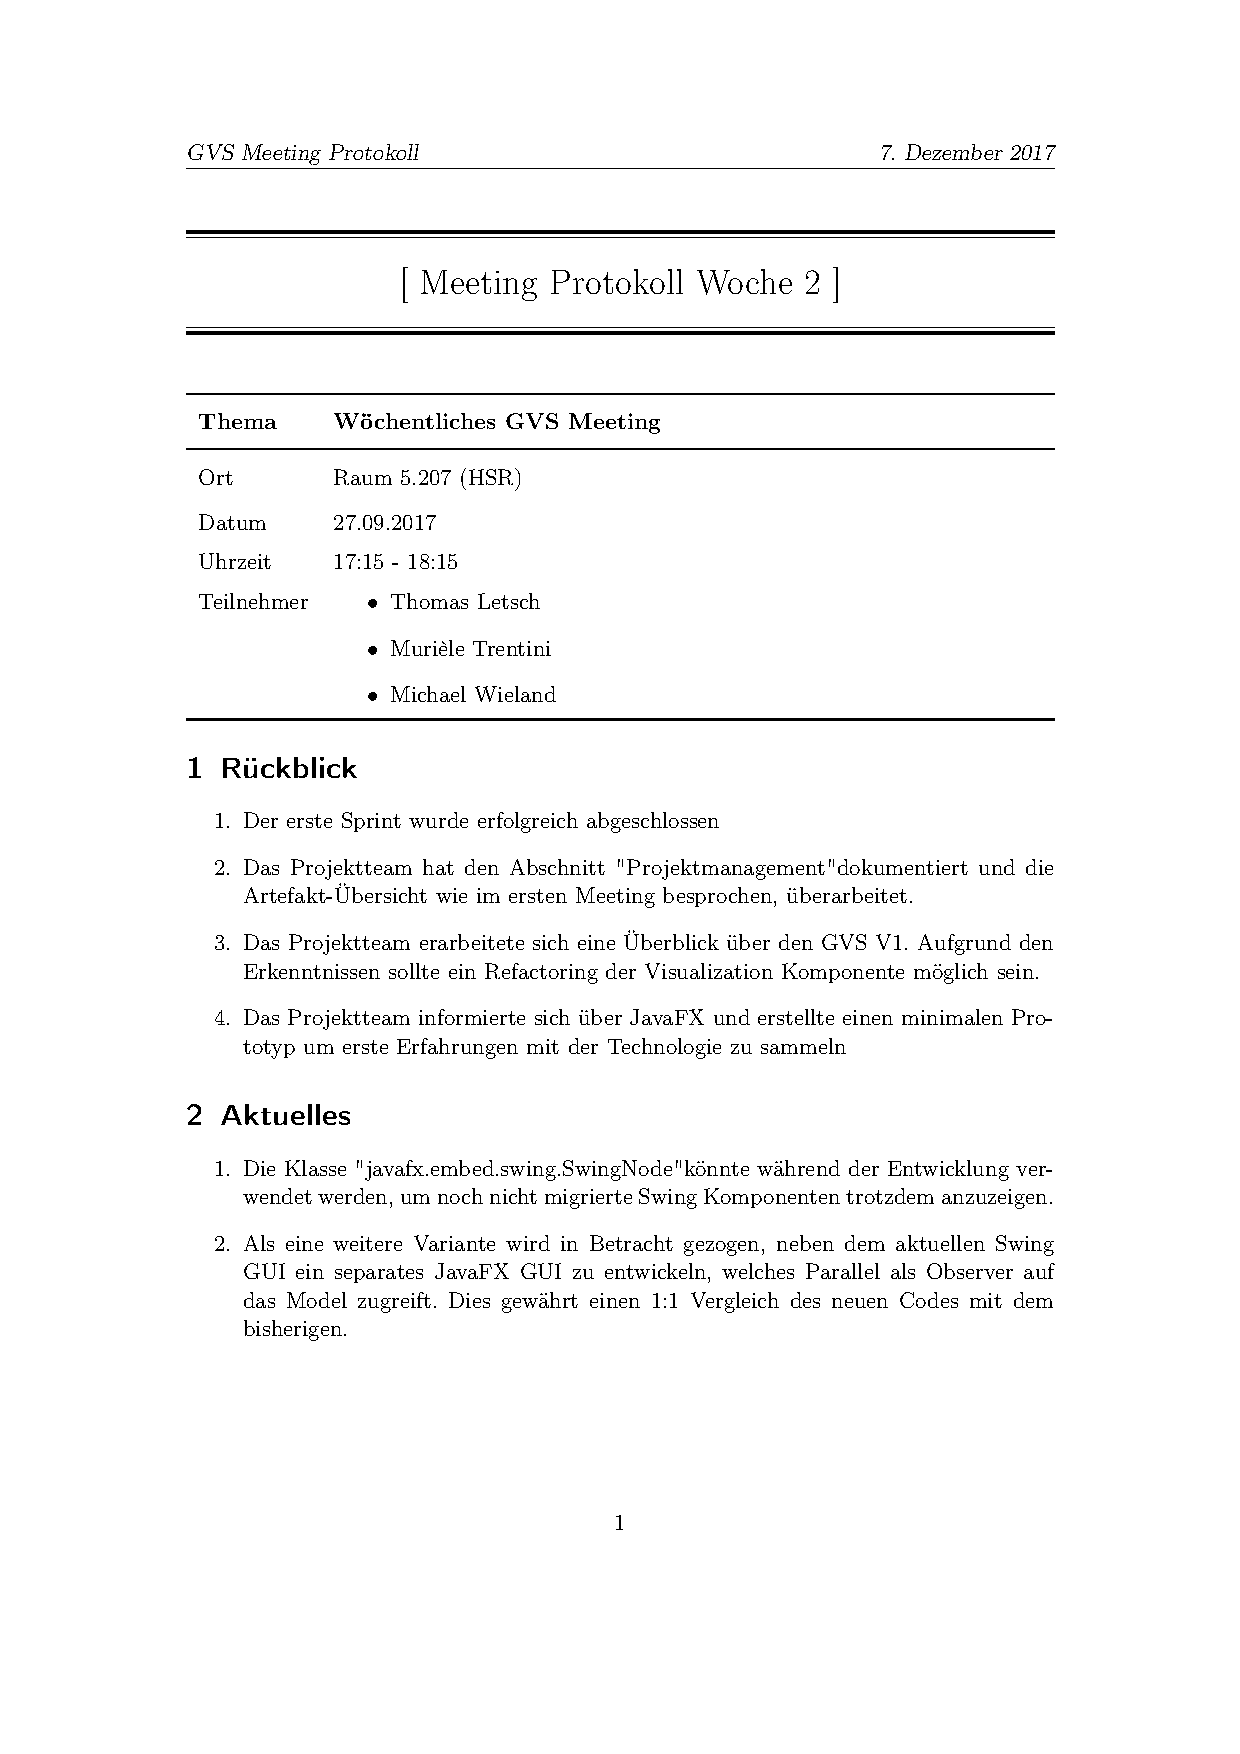
\includepdf[pages={1-}]{assets/minutes/2017-09-27.pdf}
	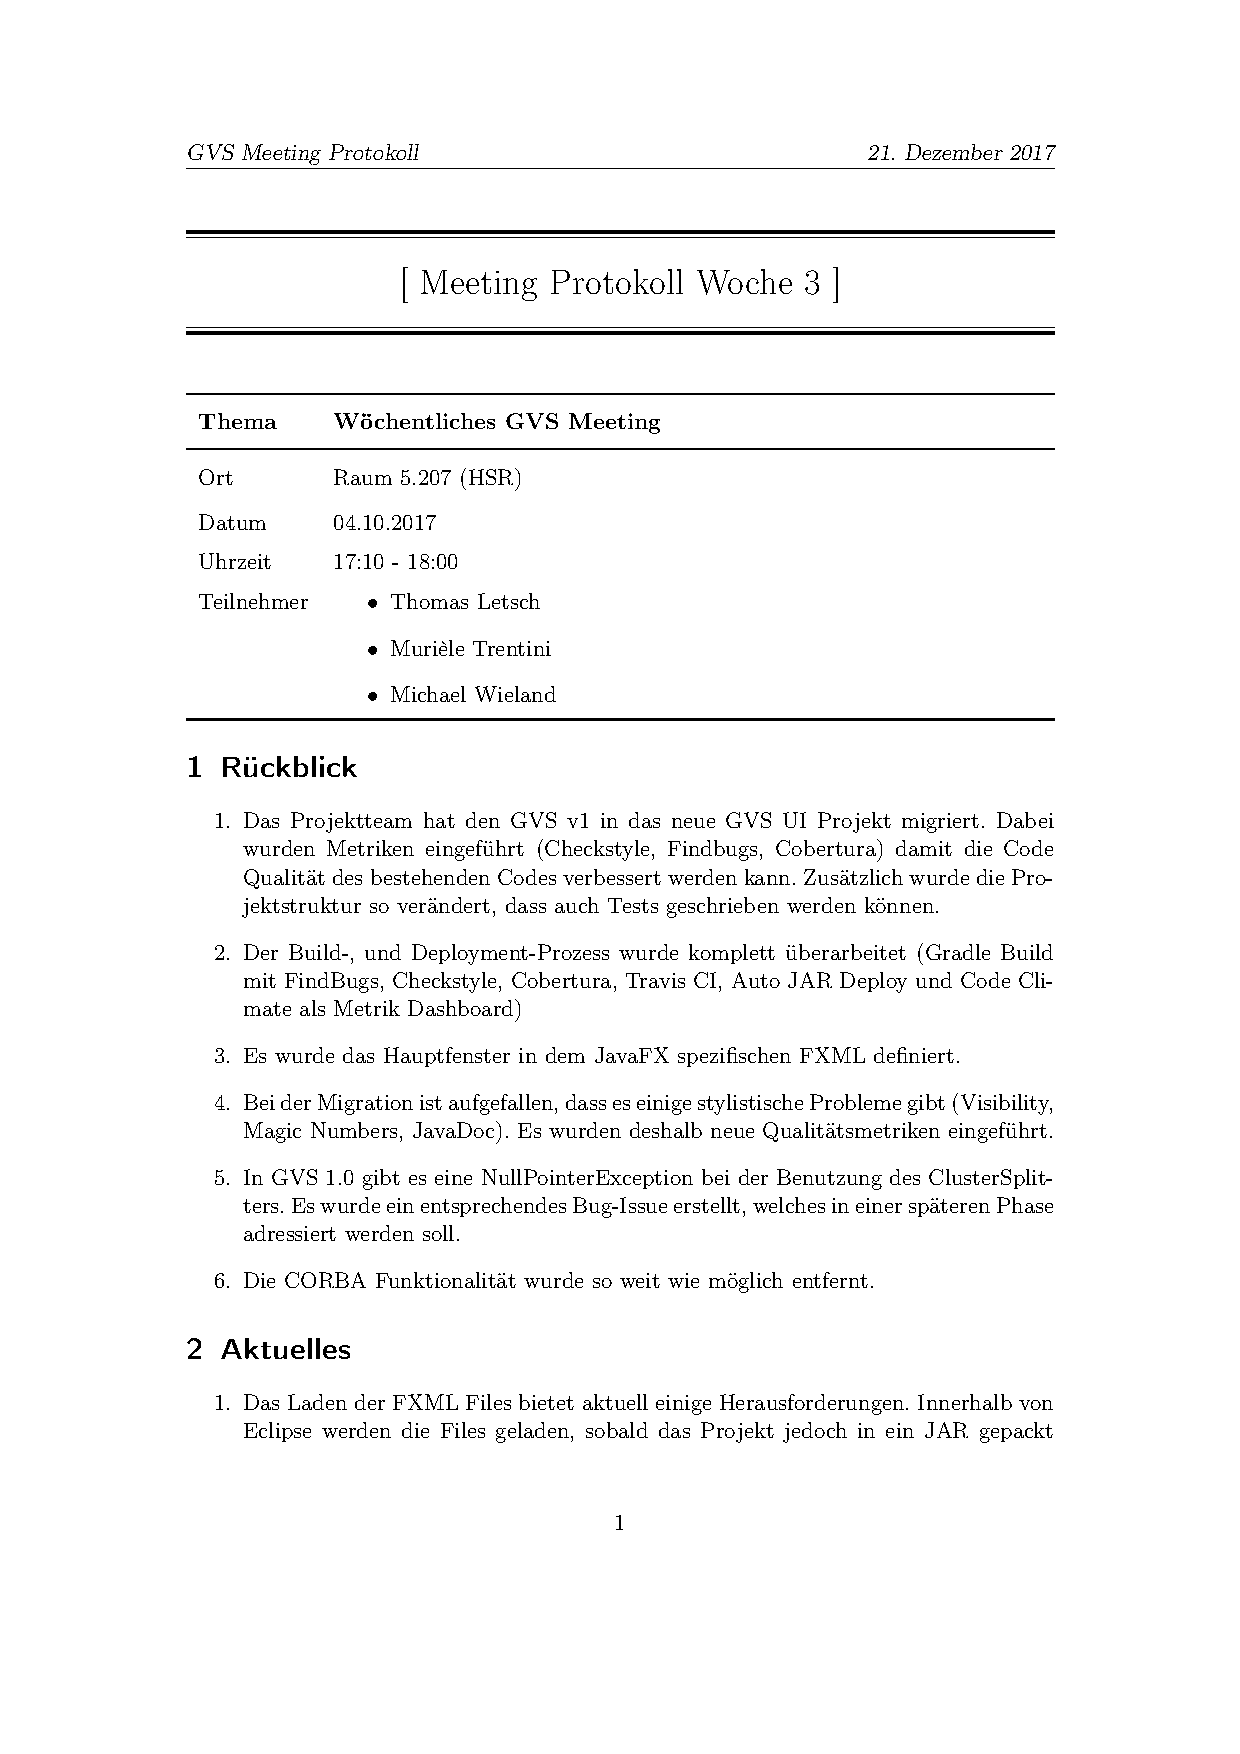
\includepdf[pages={1-}]{assets/minutes/2017-10-04.pdf}
	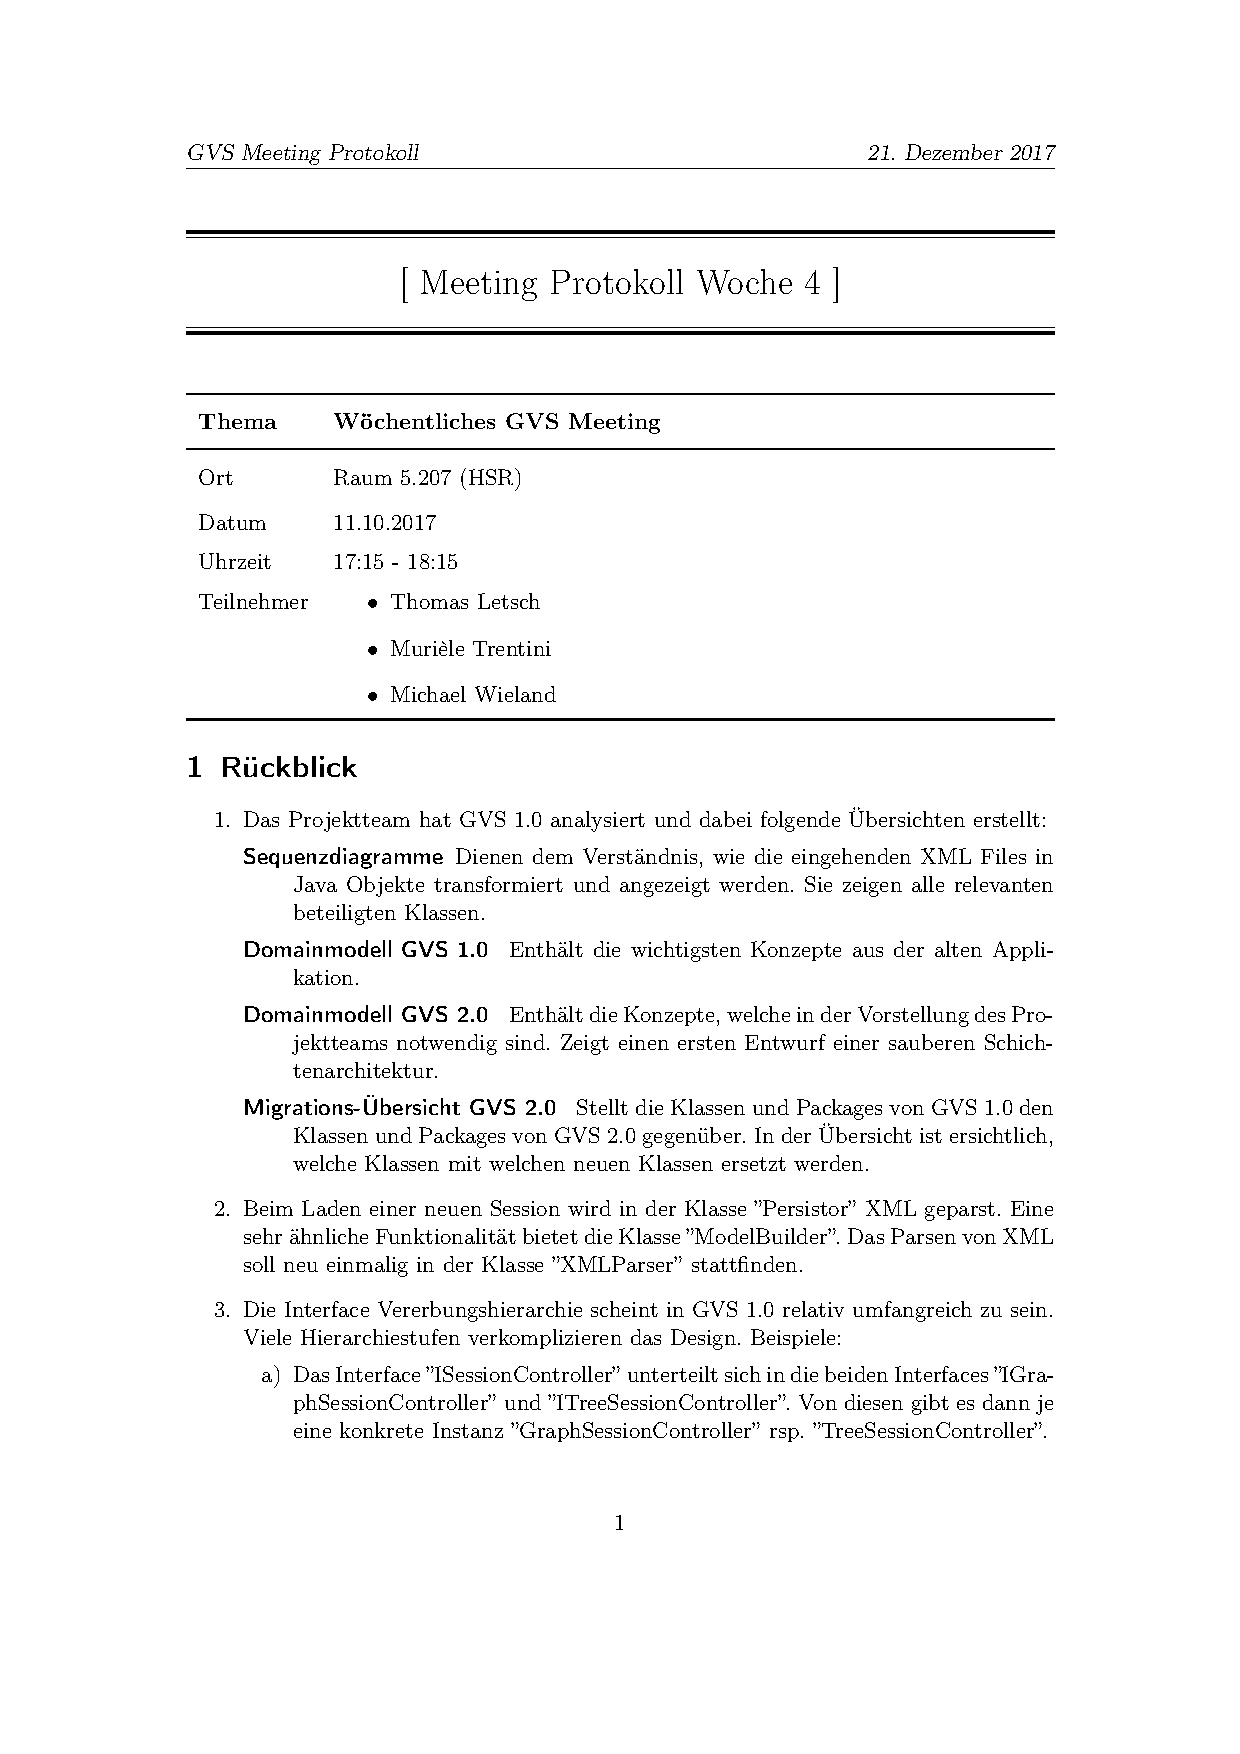
\includepdf[pages={1-}]{assets/minutes/2017-10-11.pdf}
	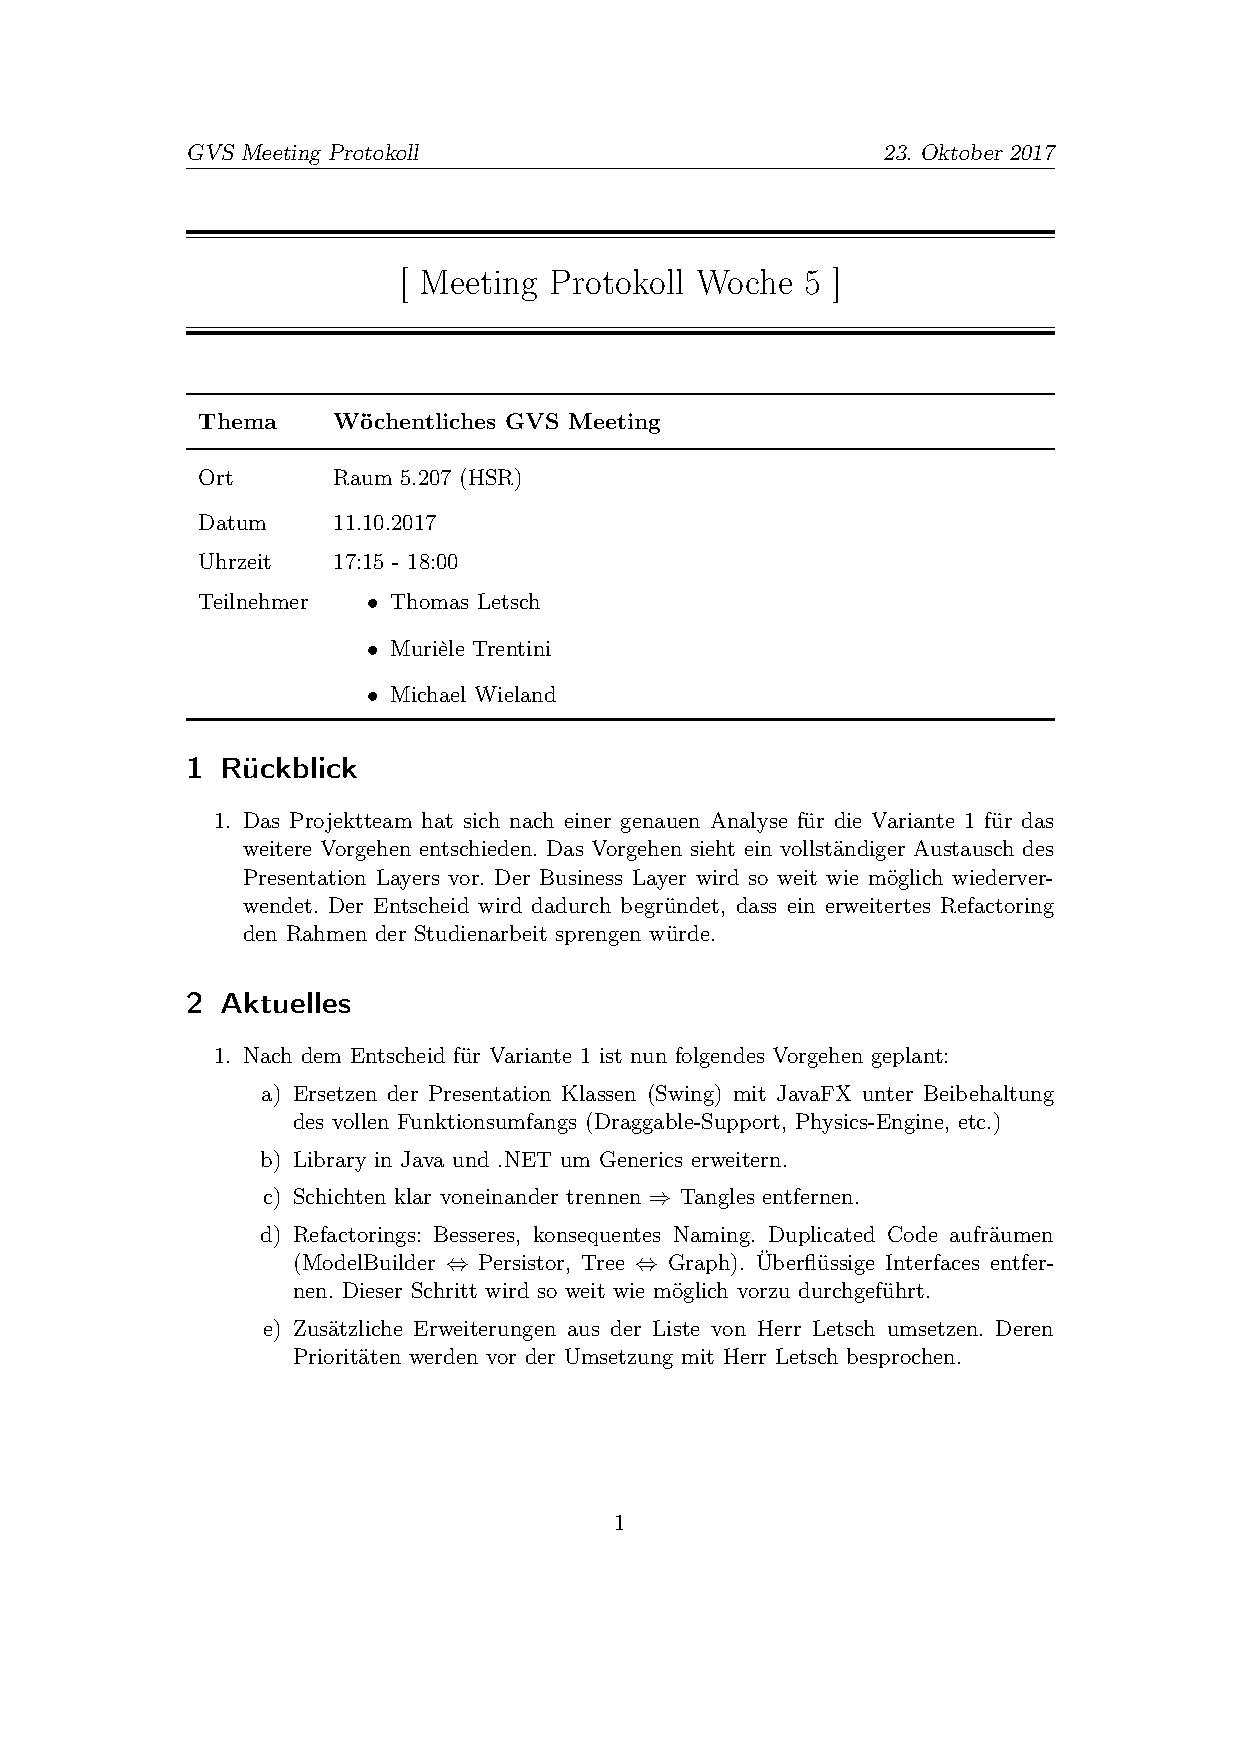
\includepdf[pages={1-}]{assets/minutes/2017-10-18.pdf}
	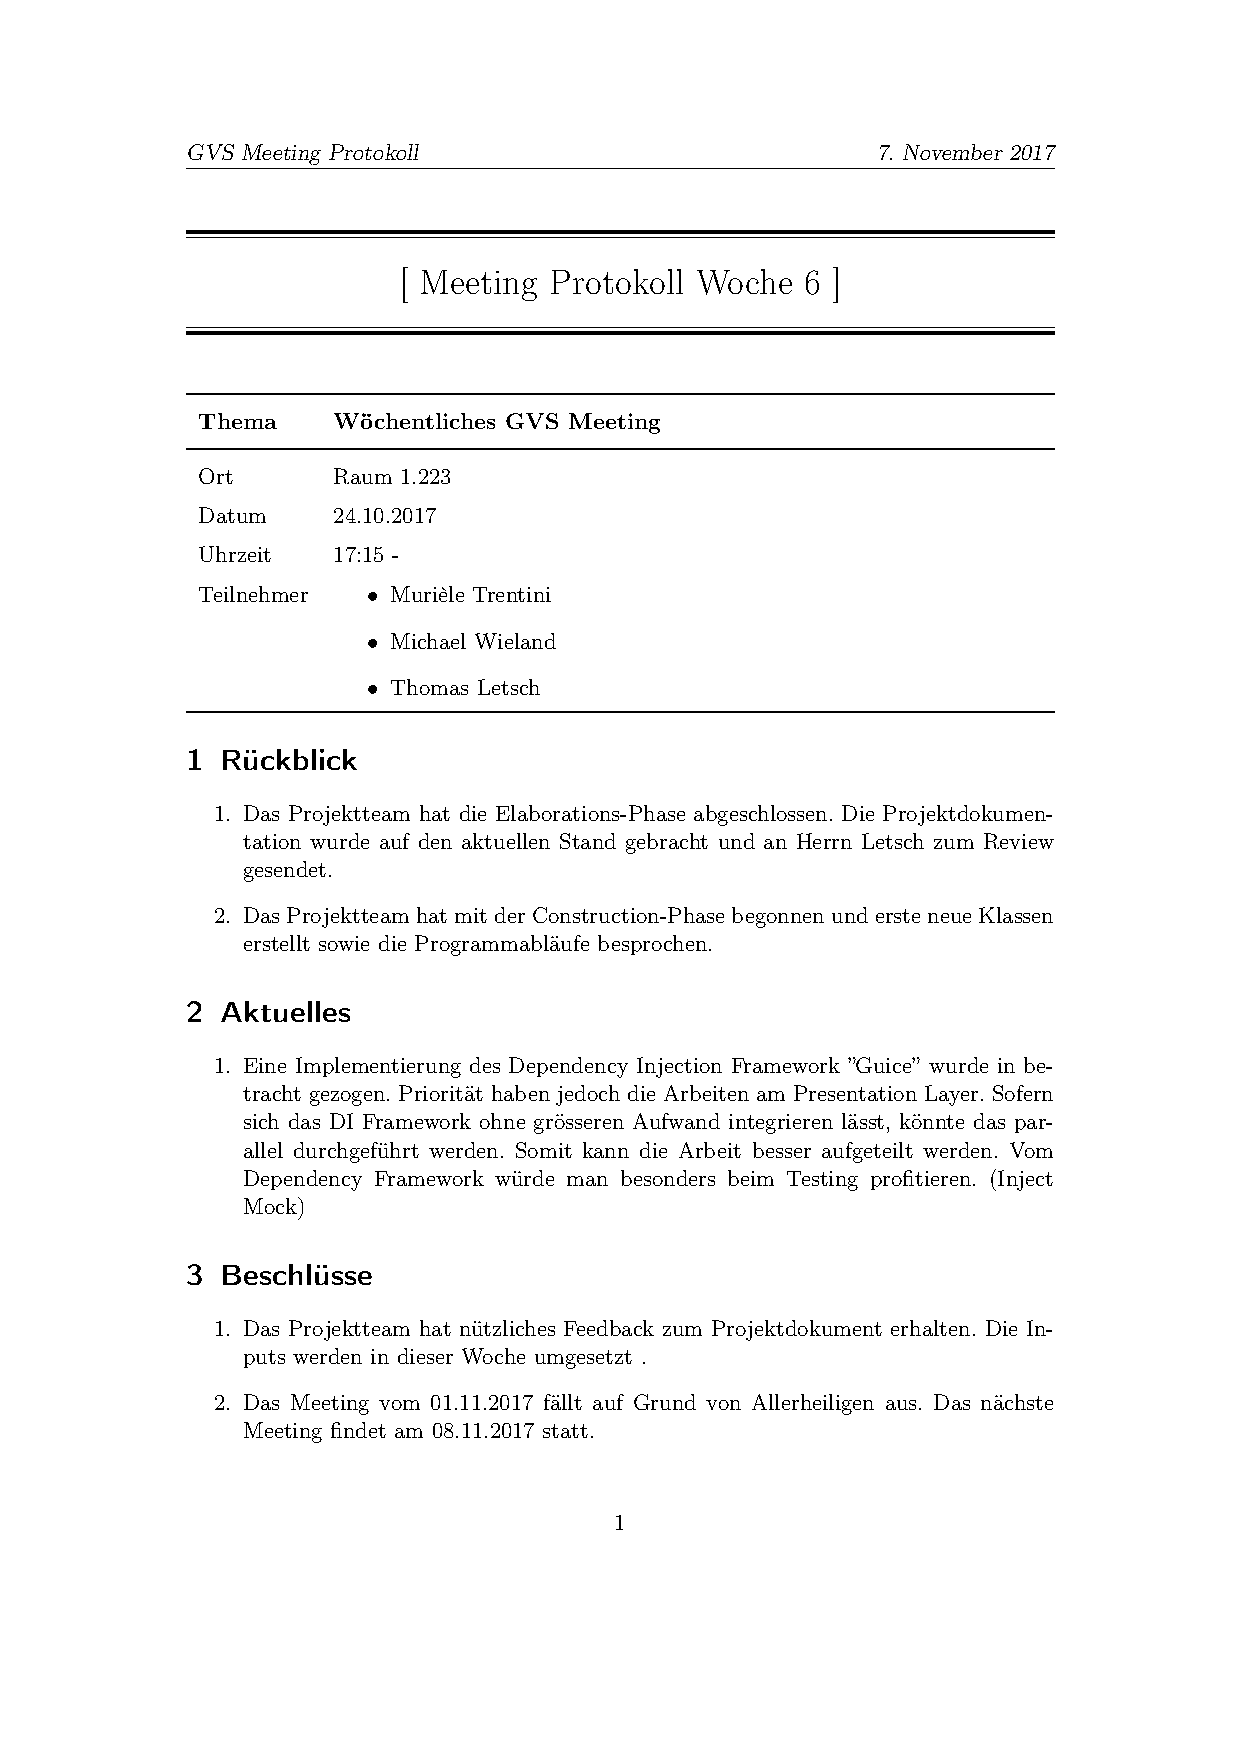
\includepdf[pages={1-}]{assets/minutes/2017-10-24.pdf}
	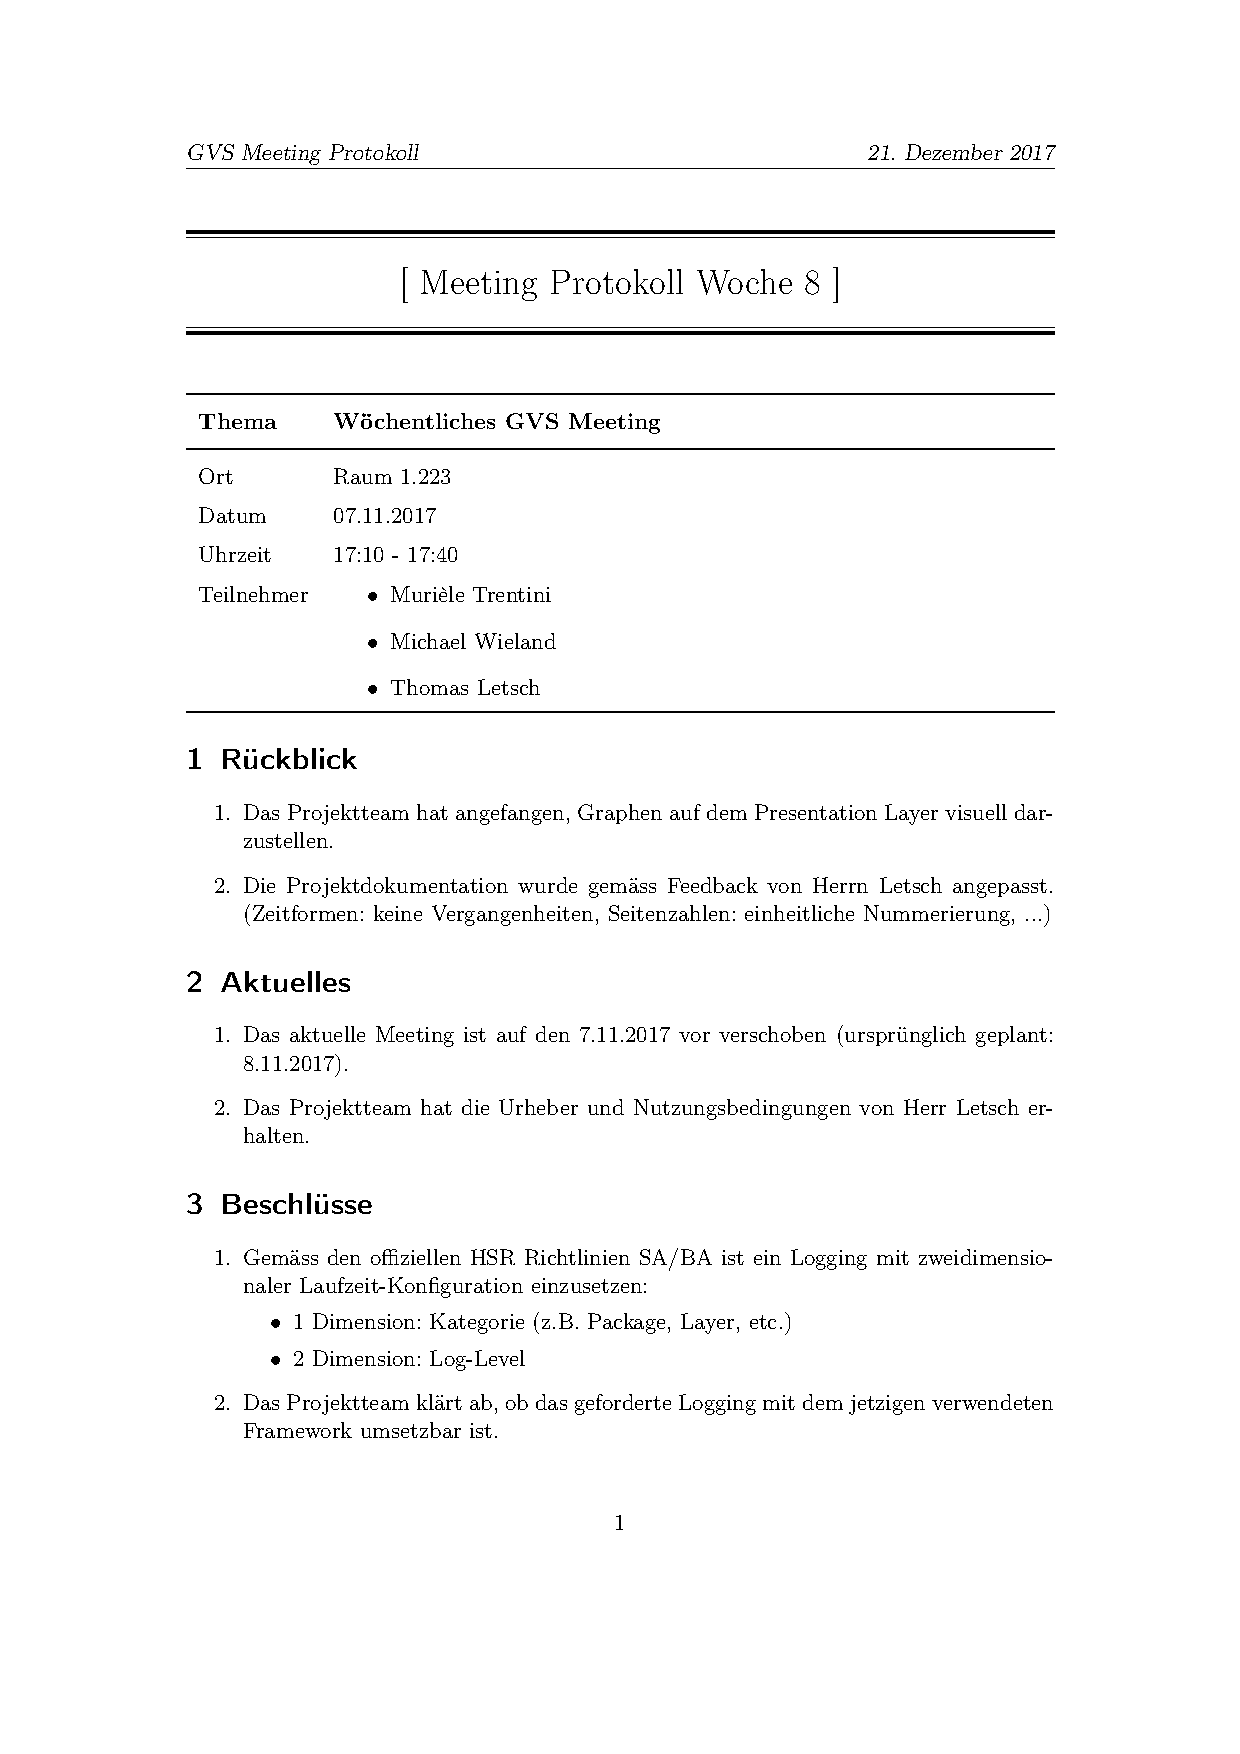
\includepdf[pages={1-}]{assets/minutes/2017-11-07.pdf}
	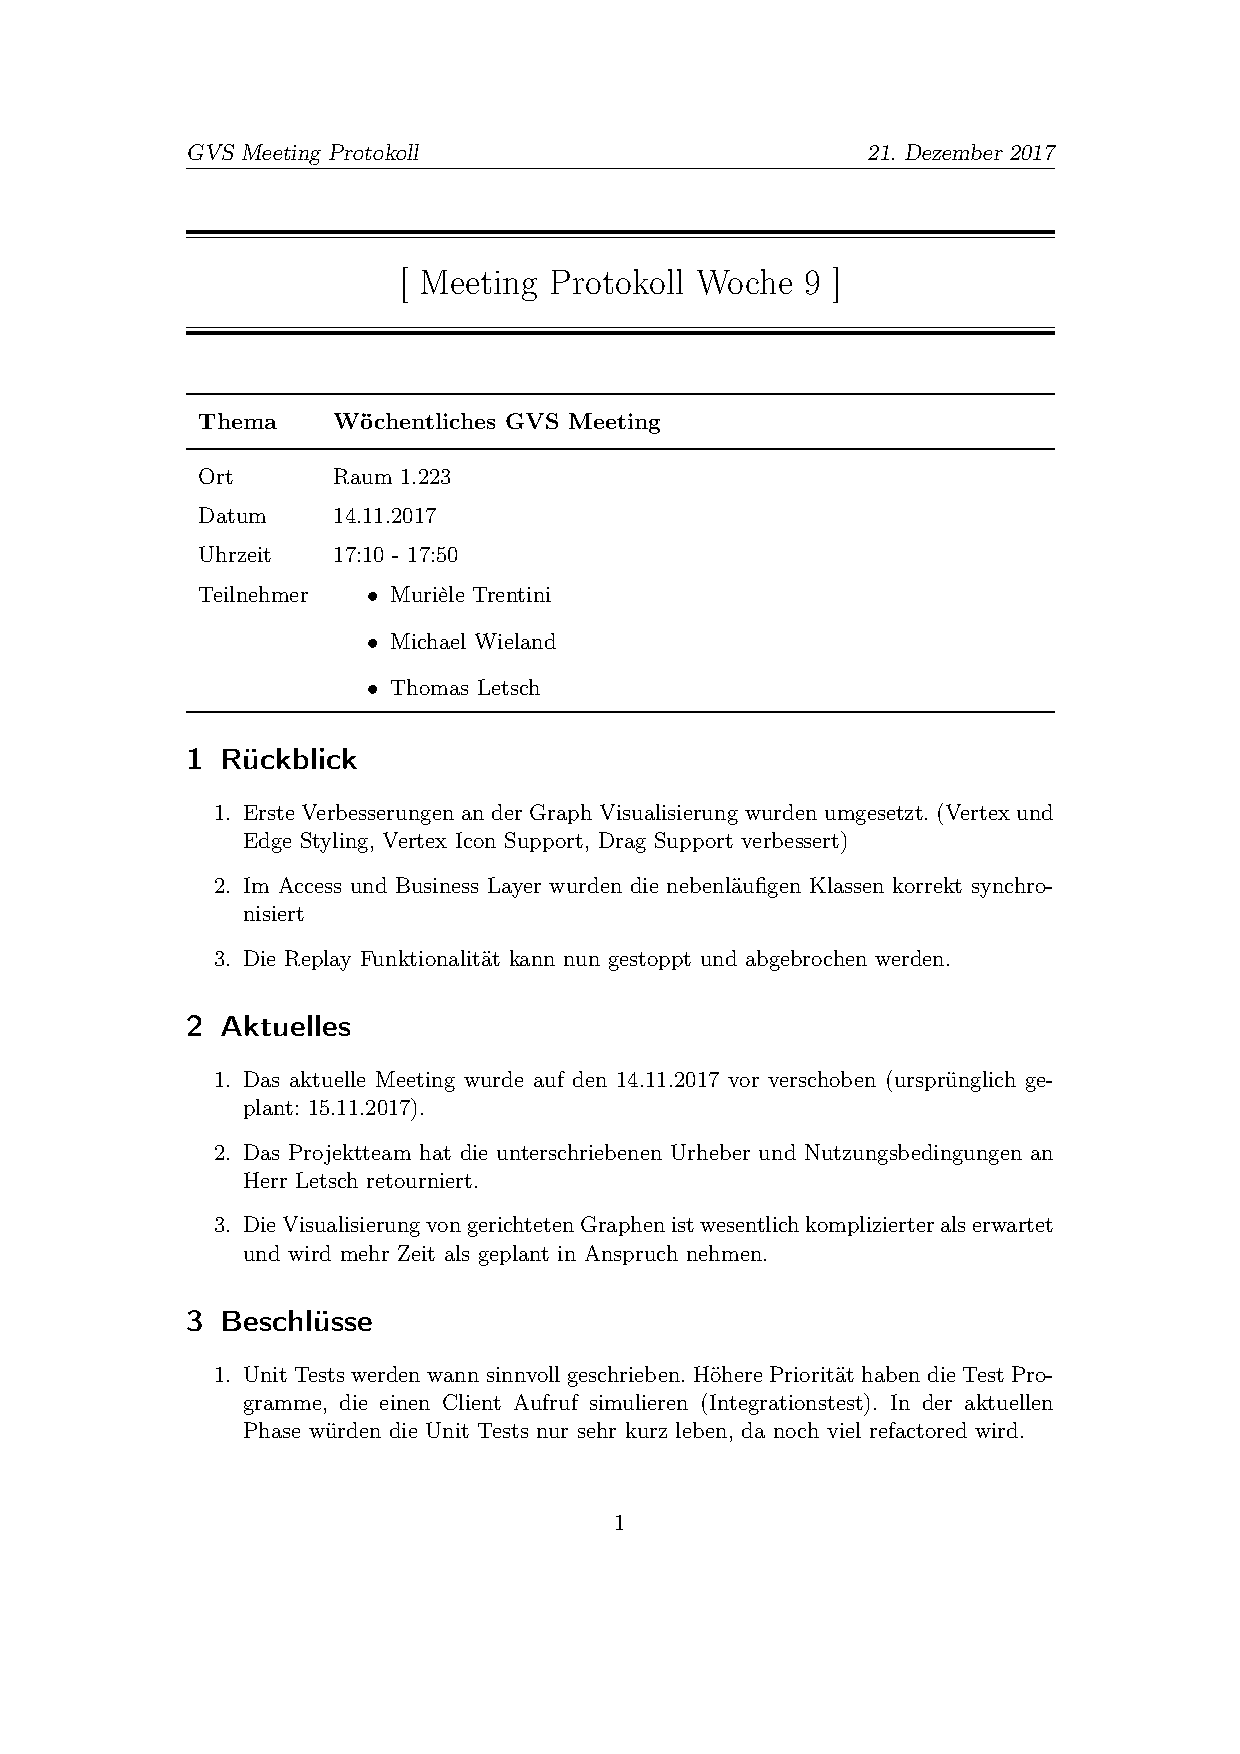
\includepdf[pages={1-}]{assets/minutes/2017-11-14.pdf}
	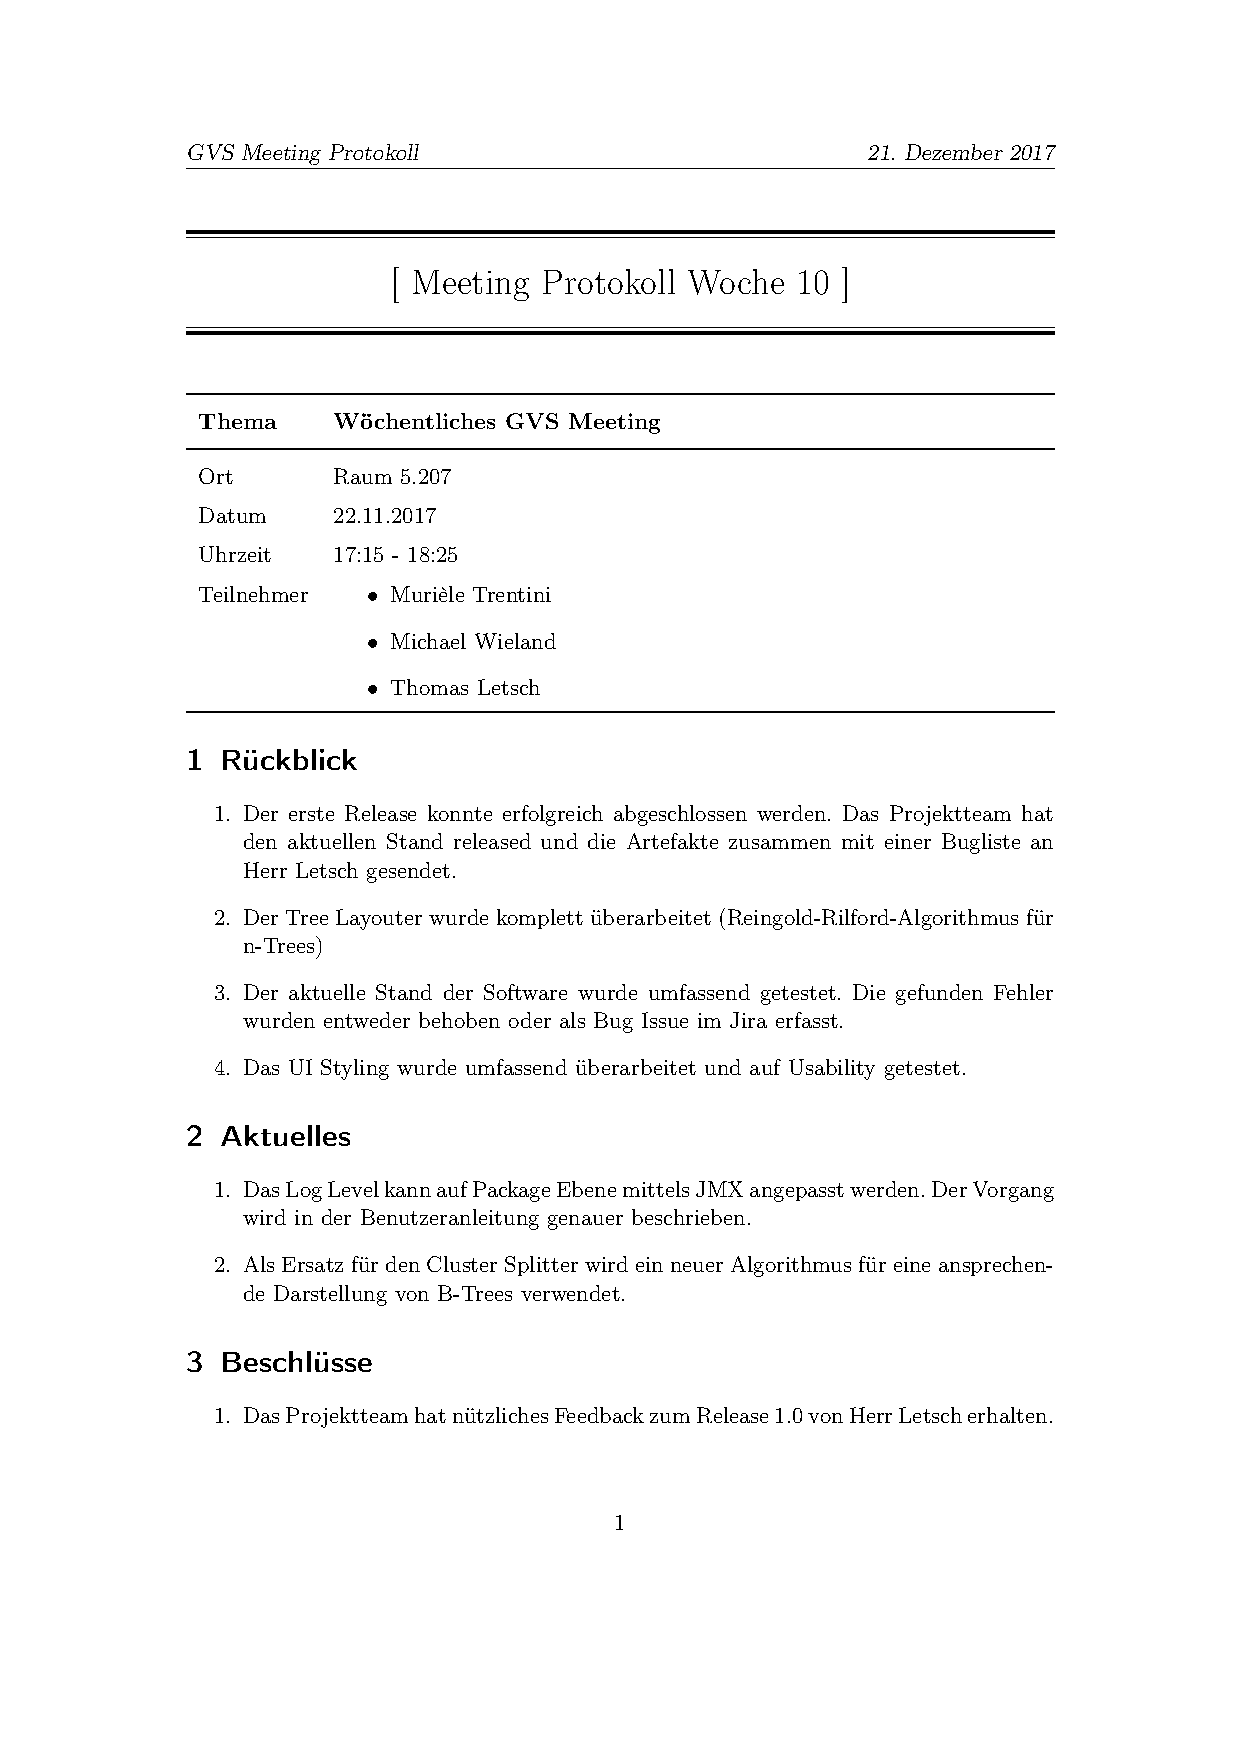
\includepdf[pages={1-}]{assets/minutes/2017-11-22.pdf}
	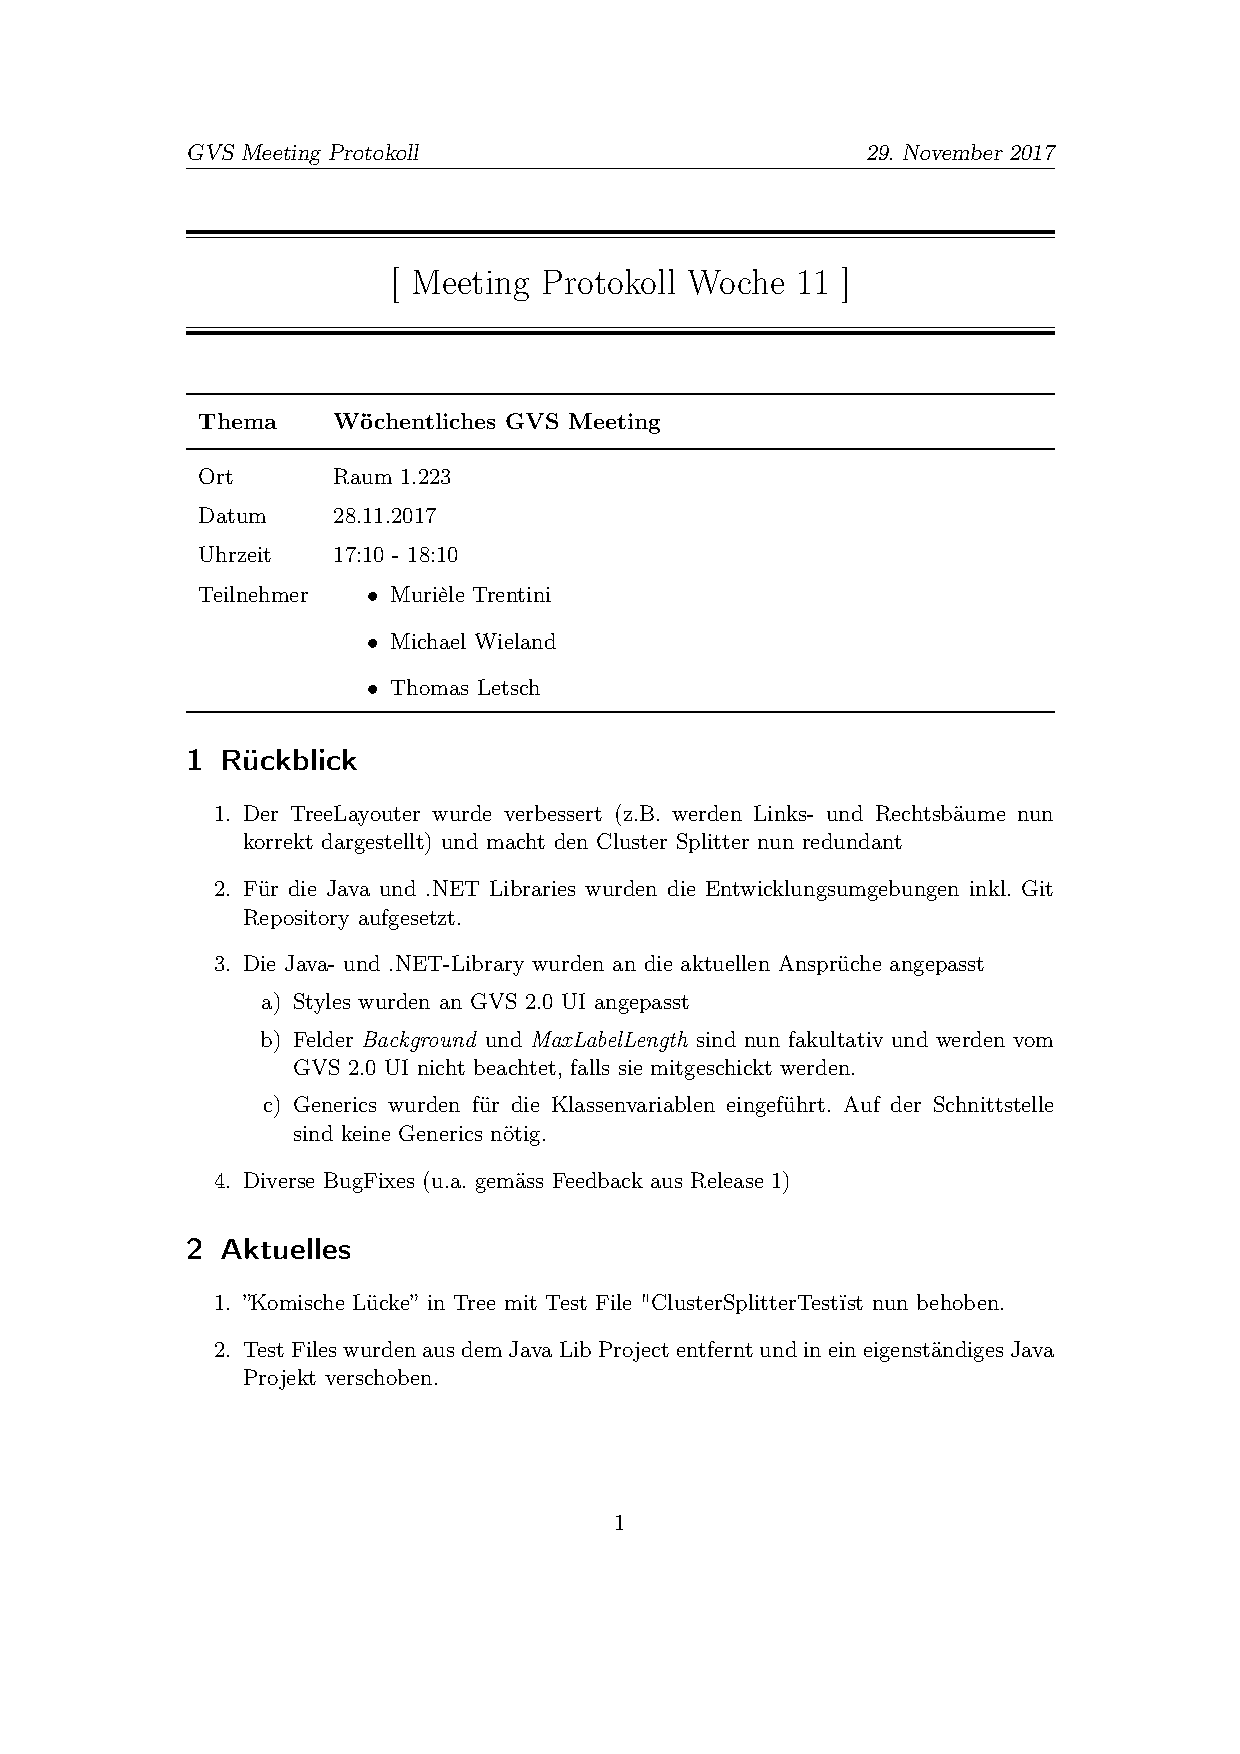
\includepdf[pages={1-}]{assets/minutes/2017-11-28.pdf}
	\includepdf[pages={1-}]{assets/minutes/2017-12-06.pdf}
	\includepdf[pages={1-}]{assets/minutes/2017-12-12.pdf}
	
	
	\chapter{Eigenständigkeitserklärung}
	
	Die folgende Seite enthält die Eigenständigkeitserklärung.
	
	\includepdf{assets/pdf/eigenstaendigkeitserklaerung}
	
	\chapter{Vereinbarung über Urheber- und Nutzungsrechte}
	Die folgende Seite enthält die Vereinbarung über Urheber- und Nutzungsrechte.
	\includepdf[pages={1}]{assets/pdf/Nutzungsbestimmung.pdf}
	
	% Glossary
	\printglossary
	\glsaddall
	
	% List of references
	\printbibliography[heading=bibintoc]
	
	{
		\hypersetup{linkcolor=black}
		\listoffigures
	}
	
	{
		\hypersetup{linkcolor=black}
		\listoftables
	}
	
\end{document}

